\documentclass[twoside]{book}

% Packages required by doxygen
\usepackage{fixltx2e}
\usepackage{calc}
\usepackage{doxygen}
\usepackage[export]{adjustbox} % also loads graphicx
\usepackage{graphicx}
\usepackage[utf8]{inputenc}
\usepackage{makeidx}
\usepackage{multicol}
\usepackage{multirow}
\PassOptionsToPackage{warn}{textcomp}
\usepackage{textcomp}
\usepackage[nointegrals]{wasysym}
\usepackage[table]{xcolor}

% Font selection
\usepackage[T1]{fontenc}
\usepackage[scaled=.90]{helvet}
\usepackage{courier}
\usepackage{amssymb}
\usepackage{sectsty}
\renewcommand{\familydefault}{\sfdefault}
\allsectionsfont{%
  \fontseries{bc}\selectfont%
  \color{darkgray}%
}
\renewcommand{\DoxyLabelFont}{%
  \fontseries{bc}\selectfont%
  \color{darkgray}%
}
\newcommand{\+}{\discretionary{\mbox{\scriptsize$\hookleftarrow$}}{}{}}

% Page & text layout
\usepackage{geometry}
\geometry{%
  a4paper,%
  top=2.5cm,%
  bottom=2.5cm,%
  left=2.5cm,%
  right=2.5cm%
}
\tolerance=750
\hfuzz=15pt
\hbadness=750
\setlength{\emergencystretch}{15pt}
\setlength{\parindent}{0cm}
\setlength{\parskip}{3ex plus 2ex minus 2ex}
\makeatletter
\renewcommand{\paragraph}{%
  \@startsection{paragraph}{4}{0ex}{-1.0ex}{1.0ex}{%
    \normalfont\normalsize\bfseries\SS@parafont%
  }%
}
\renewcommand{\subparagraph}{%
  \@startsection{subparagraph}{5}{0ex}{-1.0ex}{1.0ex}{%
    \normalfont\normalsize\bfseries\SS@subparafont%
  }%
}
\makeatother

% Headers & footers
\usepackage{fancyhdr}
\pagestyle{fancyplain}
\fancyhead[LE]{\fancyplain{}{\bfseries\thepage}}
\fancyhead[CE]{\fancyplain{}{}}
\fancyhead[RE]{\fancyplain{}{\bfseries\leftmark}}
\fancyhead[LO]{\fancyplain{}{\bfseries\rightmark}}
\fancyhead[CO]{\fancyplain{}{}}
\fancyhead[RO]{\fancyplain{}{\bfseries\thepage}}
\fancyfoot[LE]{\fancyplain{}{}}
\fancyfoot[CE]{\fancyplain{}{}}
\fancyfoot[RE]{\fancyplain{}{\bfseries\scriptsize Generated by Doxygen }}
\fancyfoot[LO]{\fancyplain{}{\bfseries\scriptsize Generated by Doxygen }}
\fancyfoot[CO]{\fancyplain{}{}}
\fancyfoot[RO]{\fancyplain{}{}}
\renewcommand{\footrulewidth}{0.4pt}
\renewcommand{\chaptermark}[1]{%
  \markboth{#1}{}%
}
\renewcommand{\sectionmark}[1]{%
  \markright{\thesection\ #1}%
}

% Indices & bibliography
\usepackage{natbib}
\usepackage[titles]{tocloft}
\setcounter{tocdepth}{3}
\setcounter{secnumdepth}{5}
\makeindex

% Hyperlinks (required, but should be loaded last)
\usepackage{ifpdf}
\ifpdf
  \usepackage[pdftex,pagebackref=true]{hyperref}
\else
  \usepackage[ps2pdf,pagebackref=true]{hyperref}
\fi
\hypersetup{%
  colorlinks=true,%
  linkcolor=blue,%
  citecolor=blue,%
  unicode%
}

% Custom commands
\newcommand{\clearemptydoublepage}{%
  \newpage{\pagestyle{empty}\cleardoublepage}%
}

\usepackage{caption}
\captionsetup{labelsep=space,justification=centering,font={bf},singlelinecheck=off,skip=4pt,position=top}

%===== C O N T E N T S =====

\begin{document}

% Titlepage & ToC
\hypersetup{pageanchor=false,
             bookmarksnumbered=true,
             pdfencoding=unicode
            }
\pagenumbering{roman}
\begin{titlepage}
\vspace*{7cm}
\begin{center}%
{\Large A\+C\+FD }\\
\vspace*{1cm}
{\large Generated by Doxygen 1.8.11}\\
\end{center}
\end{titlepage}
\clearemptydoublepage
\tableofcontents
\clearemptydoublepage
\pagenumbering{arabic}
\hypersetup{pageanchor=true}

%--- Begin generated contents ---
\chapter{Hierarchical Index}
\section{Class Hierarchy}
This inheritance list is sorted roughly, but not completely, alphabetically\+:\begin{DoxyCompactList}
\item \contentsline{section}{Boundary}{\pageref{class_boundary}}{}
\begin{DoxyCompactList}
\item \contentsline{section}{Boundary\+\_\+\+Periodic}{\pageref{class_boundary___periodic}}{}
\end{DoxyCompactList}
\item \contentsline{section}{Control}{\pageref{class_control}}{}
\item \contentsline{section}{Control\+:\+:Control\+Pair}{\pageref{struct_control_1_1_control_pair}}{}
\item \contentsline{section}{Driver}{\pageref{class_driver}}{}
\begin{DoxyCompactList}
\item \contentsline{section}{Driver\+\_\+\+Standard}{\pageref{class_driver___standard}}{}
\end{DoxyCompactList}
\item \contentsline{section}{Fluxes}{\pageref{class_fluxes}}{}
\begin{DoxyCompactList}
\item \contentsline{section}{Fluxes\+\_\+\+Advection}{\pageref{class_fluxes___advection}}{}
\end{DoxyCompactList}
\item \contentsline{section}{Gnuplot}{\pageref{class_gnuplot}}{}
\item \contentsline{section}{Grid}{\pageref{class_grid}}{}
\item \contentsline{section}{Init}{\pageref{class_init}}{}
\begin{DoxyCompactList}
\item \contentsline{section}{Init\+\_\+\+Advection}{\pageref{class_init___advection}}{}
\end{DoxyCompactList}
\item \contentsline{section}{Plot}{\pageref{class_plot}}{}
\begin{DoxyCompactList}
\item \contentsline{section}{Plot\+\_\+\+Advection}{\pageref{class_plot___advection}}{}
\end{DoxyCompactList}
\item \contentsline{section}{Postprocess}{\pageref{class_postprocess}}{}
\begin{DoxyCompactList}
\item \contentsline{section}{Postprocess\+\_\+\+Advection}{\pageref{class_postprocess___advection}}{}
\item \contentsline{section}{Postprocess\+\_\+\+Empty}{\pageref{class_postprocess___empty}}{}
\end{DoxyCompactList}
\item runtime\+\_\+error\begin{DoxyCompactList}
\item \contentsline{section}{Gnuplot\+Exception}{\pageref{class_gnuplot_exception}}{}
\end{DoxyCompactList}
\item \contentsline{section}{Setup}{\pageref{class_setup}}{}
\begin{DoxyCompactList}
\item \contentsline{section}{Setup\+\_\+\+Advection}{\pageref{class_setup___advection}}{}
\end{DoxyCompactList}
\item \contentsline{section}{Source}{\pageref{class_source}}{}
\begin{DoxyCompactList}
\item \contentsline{section}{Source\+\_\+\+Empty}{\pageref{class_source___empty}}{}
\end{DoxyCompactList}
\item \contentsline{section}{Time}{\pageref{class_time}}{}
\item \contentsline{section}{Update}{\pageref{class_update}}{}
\begin{DoxyCompactList}
\item \contentsline{section}{Update\+\_\+\+Standard}{\pageref{class_update___standard}}{}
\end{DoxyCompactList}
\end{DoxyCompactList}

\chapter{Class Index}
\section{Class List}
Here are the classes, structs, unions and interfaces with brief descriptions\+:\begin{DoxyCompactList}
\item\contentsline{section}{\hyperlink{class_boundary}{Boundary} \\*Abstract class for the computation of boundary fluxes }{\pageref{class_boundary}}{}
\item\contentsline{section}{\hyperlink{class_boundary___periodic}{Boundary\+\_\+\+Periodic} \\*Class for the computation of boundary fluxes for a periodic boundary condition }{\pageref{class_boundary___periodic}}{}
\item\contentsline{section}{\hyperlink{class_control}{Control} \\*Map that holds the contents of a control file }{\pageref{class_control}}{}
\item\contentsline{section}{\hyperlink{struct_control_1_1_control_pair}{Control\+::\+Control\+Pair} }{\pageref{struct_control_1_1_control_pair}}{}
\item\contentsline{section}{\hyperlink{class_driver}{Driver} \\*Abstract class for a simulation code driver }{\pageref{class_driver}}{}
\item\contentsline{section}{\hyperlink{class_driver___standard}{Driver\+\_\+\+Standard} \\*\hyperlink{class_driver}{Driver} for numerical simulation of conservation laws }{\pageref{class_driver___standard}}{}
\item\contentsline{section}{\hyperlink{class_fluxes}{Fluxes} \\*Class for the computation of numerical fluxes over cell interfaces for a given conservation law }{\pageref{class_fluxes}}{}
\item\contentsline{section}{\hyperlink{class_fluxes___advection}{Fluxes\+\_\+\+Advection} \\*Computation of fluxes for the linear advection-\/diffusion equation }{\pageref{class_fluxes___advection}}{}
\item\contentsline{section}{\hyperlink{class_gnuplot}{Gnuplot} }{\pageref{class_gnuplot}}{}
\item\contentsline{section}{\hyperlink{class_gnuplot_exception}{Gnuplot\+Exception} }{\pageref{class_gnuplot_exception}}{}
\item\contentsline{section}{\hyperlink{class_grid}{Grid} \\*Class for a 3D Cartesian grid with associated fields and coefficients }{\pageref{class_grid}}{}
\item\contentsline{section}{\hyperlink{class_init}{Init} \\*Abstract class for the definition of initial conditions for fields defined on a \hyperlink{class_grid}{Grid} object }{\pageref{class_init}}{}
\item\contentsline{section}{\hyperlink{class_init___advection}{Init\+\_\+\+Advection} \\*Initial condition for the linear advection-\/diffusion equation }{\pageref{class_init___advection}}{}
\item\contentsline{section}{\hyperlink{class_plot}{Plot} \\*Abstract class for plotting simulation results }{\pageref{class_plot}}{}
\item\contentsline{section}{\hyperlink{class_plot___advection}{Plot\+\_\+\+Advection} \\*Plotting class for the linear advection-\/diffusion equation }{\pageref{class_plot___advection}}{}
\item\contentsline{section}{\hyperlink{class_postprocess}{Postprocess} \\*Abstract class for postprocessing simulation results }{\pageref{class_postprocess}}{}
\item\contentsline{section}{\hyperlink{class_postprocess___advection}{Postprocess\+\_\+\+Advection} \\*Postprocessing class for the linear advection-\/diffusion equation }{\pageref{class_postprocess___advection}}{}
\item\contentsline{section}{\hyperlink{class_postprocess___empty}{Postprocess\+\_\+\+Empty} \\*Empty postprocessing class (does nothing) }{\pageref{class_postprocess___empty}}{}
\item\contentsline{section}{\hyperlink{class_setup}{Setup} \\*Class for the simulation setup }{\pageref{class_setup}}{}
\item\contentsline{section}{\hyperlink{class_setup___advection}{Setup\+\_\+\+Advection} \\*Simulation setup for the linear advection-\/diffusion equation }{\pageref{class_setup___advection}}{}
\item\contentsline{section}{\hyperlink{class_source}{Source} \\*Abstract class for a source term that is applied to a \hyperlink{class_grid}{Grid} object }{\pageref{class_source}}{}
\item\contentsline{section}{\hyperlink{class_source___empty}{Source\+\_\+\+Empty} \\*Empty source, i.\+e., the source term equals zero }{\pageref{class_source___empty}}{}
\item\contentsline{section}{\hyperlink{class_time}{Time} \\*Class for running time loops }{\pageref{class_time}}{}
\item\contentsline{section}{\hyperlink{class_update}{Update} \\*Abstract class for the update of a grid object during a time loop }{\pageref{class_update}}{}
\item\contentsline{section}{\hyperlink{class_update___standard}{Update\+\_\+\+Standard} \\*Class for the update of a grid object during a time loop, using standard flux differencing }{\pageref{class_update___standard}}{}
\end{DoxyCompactList}

\chapter{File Index}
\section{File List}
Here is a list of all files with brief descriptions\+:\begin{DoxyCompactList}
\item\contentsline{section}{/home/doberle/\+Advanced C\+F\+D/acfd/\+Code/\hyperlink{boundary_8h}{boundary.\+h} }{\pageref{boundary_8h}}{}
\item\contentsline{section}{/home/doberle/\+Advanced C\+F\+D/acfd/\+Code/\hyperlink{boundary__periodic_8h}{boundary\+\_\+periodic.\+h} }{\pageref{boundary__periodic_8h}}{}
\item\contentsline{section}{/home/doberle/\+Advanced C\+F\+D/acfd/\+Code/\hyperlink{control_8cpp}{control.\+cpp} }{\pageref{control_8cpp}}{}
\item\contentsline{section}{/home/doberle/\+Advanced C\+F\+D/acfd/\+Code/\hyperlink{control_8h}{control.\+h} }{\pageref{control_8h}}{}
\item\contentsline{section}{/home/doberle/\+Advanced C\+F\+D/acfd/\+Code/\hyperlink{driver_8h}{driver.\+h} }{\pageref{driver_8h}}{}
\item\contentsline{section}{/home/doberle/\+Advanced C\+F\+D/acfd/\+Code/\hyperlink{driver__standard_8cpp}{driver\+\_\+standard.\+cpp} }{\pageref{driver__standard_8cpp}}{}
\item\contentsline{section}{/home/doberle/\+Advanced C\+F\+D/acfd/\+Code/\hyperlink{driver__standard_8h}{driver\+\_\+standard.\+h} }{\pageref{driver__standard_8h}}{}
\item\contentsline{section}{/home/doberle/\+Advanced C\+F\+D/acfd/\+Code/\hyperlink{fluxes_8cpp}{fluxes.\+cpp} }{\pageref{fluxes_8cpp}}{}
\item\contentsline{section}{/home/doberle/\+Advanced C\+F\+D/acfd/\+Code/\hyperlink{fluxes_8h}{fluxes.\+h} }{\pageref{fluxes_8h}}{}
\item\contentsline{section}{/home/doberle/\+Advanced C\+F\+D/acfd/\+Code/\hyperlink{fluxes__advection_8cpp}{fluxes\+\_\+advection.\+cpp} }{\pageref{fluxes__advection_8cpp}}{}
\item\contentsline{section}{/home/doberle/\+Advanced C\+F\+D/acfd/\+Code/\hyperlink{fluxes__advection_8h}{fluxes\+\_\+advection.\+h} }{\pageref{fluxes__advection_8h}}{}
\item\contentsline{section}{/home/doberle/\+Advanced C\+F\+D/acfd/\+Code/\hyperlink{gnuplot__i_8cpp}{gnuplot\+\_\+i.\+cpp} }{\pageref{gnuplot__i_8cpp}}{}
\item\contentsline{section}{/home/doberle/\+Advanced C\+F\+D/acfd/\+Code/\hyperlink{gnuplot__i_8h}{gnuplot\+\_\+i.\+h} }{\pageref{gnuplot__i_8h}}{}
\item\contentsline{section}{/home/doberle/\+Advanced C\+F\+D/acfd/\+Code/\hyperlink{grid_8cpp}{grid.\+cpp} }{\pageref{grid_8cpp}}{}
\item\contentsline{section}{/home/doberle/\+Advanced C\+F\+D/acfd/\+Code/\hyperlink{grid_8h}{grid.\+h} }{\pageref{grid_8h}}{}
\item\contentsline{section}{/home/doberle/\+Advanced C\+F\+D/acfd/\+Code/\hyperlink{init_8h}{init.\+h} }{\pageref{init_8h}}{}
\item\contentsline{section}{/home/doberle/\+Advanced C\+F\+D/acfd/\+Code/\hyperlink{init__advection_8cpp}{init\+\_\+advection.\+cpp} }{\pageref{init__advection_8cpp}}{}
\item\contentsline{section}{/home/doberle/\+Advanced C\+F\+D/acfd/\+Code/\hyperlink{init__advection_8h}{init\+\_\+advection.\+h} }{\pageref{init__advection_8h}}{}
\item\contentsline{section}{/home/doberle/\+Advanced C\+F\+D/acfd/\+Code/\hyperlink{main_8cpp}{main.\+cpp} }{\pageref{main_8cpp}}{}
\item\contentsline{section}{/home/doberle/\+Advanced C\+F\+D/acfd/\+Code/\hyperlink{plot_8h}{plot.\+h} }{\pageref{plot_8h}}{}
\item\contentsline{section}{/home/doberle/\+Advanced C\+F\+D/acfd/\+Code/\hyperlink{plot__advection_8cpp}{plot\+\_\+advection.\+cpp} }{\pageref{plot__advection_8cpp}}{}
\item\contentsline{section}{/home/doberle/\+Advanced C\+F\+D/acfd/\+Code/\hyperlink{plot__advection_8h}{plot\+\_\+advection.\+h} }{\pageref{plot__advection_8h}}{}
\item\contentsline{section}{/home/doberle/\+Advanced C\+F\+D/acfd/\+Code/\hyperlink{postprocess_8h}{postprocess.\+h} }{\pageref{postprocess_8h}}{}
\item\contentsline{section}{/home/doberle/\+Advanced C\+F\+D/acfd/\+Code/\hyperlink{postprocess__advection_8cpp}{postprocess\+\_\+advection.\+cpp} }{\pageref{postprocess__advection_8cpp}}{}
\item\contentsline{section}{/home/doberle/\+Advanced C\+F\+D/acfd/\+Code/\hyperlink{postprocess__advection_8h}{postprocess\+\_\+advection.\+h} }{\pageref{postprocess__advection_8h}}{}
\item\contentsline{section}{/home/doberle/\+Advanced C\+F\+D/acfd/\+Code/\hyperlink{postprocess__empty_8h}{postprocess\+\_\+empty.\+h} }{\pageref{postprocess__empty_8h}}{}
\item\contentsline{section}{/home/doberle/\+Advanced C\+F\+D/acfd/\+Code/\hyperlink{setup_8h}{setup.\+h} }{\pageref{setup_8h}}{}
\item\contentsline{section}{/home/doberle/\+Advanced C\+F\+D/acfd/\+Code/\hyperlink{setup__advection_8h}{setup\+\_\+advection.\+h} }{\pageref{setup__advection_8h}}{}
\item\contentsline{section}{/home/doberle/\+Advanced C\+F\+D/acfd/\+Code/\hyperlink{source_8h}{source.\+h} }{\pageref{source_8h}}{}
\item\contentsline{section}{/home/doberle/\+Advanced C\+F\+D/acfd/\+Code/\hyperlink{source__empty_8h}{source\+\_\+empty.\+h} }{\pageref{source__empty_8h}}{}
\item\contentsline{section}{/home/doberle/\+Advanced C\+F\+D/acfd/\+Code/\hyperlink{time_8h}{time.\+h} }{\pageref{time_8h}}{}
\item\contentsline{section}{/home/doberle/\+Advanced C\+F\+D/acfd/\+Code/\hyperlink{update_8h}{update.\+h} }{\pageref{update_8h}}{}
\item\contentsline{section}{/home/doberle/\+Advanced C\+F\+D/acfd/\+Code/\hyperlink{update__standard_8cpp}{update\+\_\+standard.\+cpp} }{\pageref{update__standard_8cpp}}{}
\item\contentsline{section}{/home/doberle/\+Advanced C\+F\+D/acfd/\+Code/\hyperlink{update__standard_8h}{update\+\_\+standard.\+h} }{\pageref{update__standard_8h}}{}
\end{DoxyCompactList}

\chapter{Class Documentation}
\hypertarget{class_boundary}{}\section{Boundary Class Reference}
\label{class_boundary}\index{Boundary@{Boundary}}


Abstract class for the computation of boundary fluxes.  




{\ttfamily \#include $<$boundary.\+h$>$}

Inheritance diagram for Boundary\+:\begin{figure}[H]
\begin{center}
\leavevmode
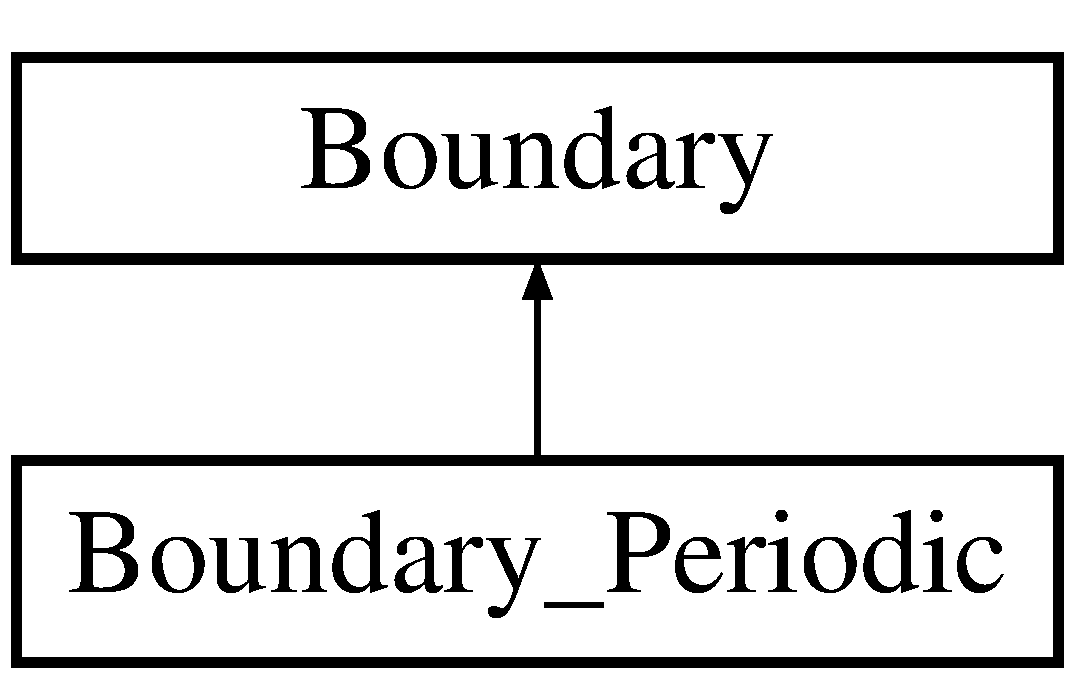
\includegraphics[height=2.000000cm]{class_boundary}
\end{center}
\end{figure}
\subsection*{Public Member Functions}
\begin{DoxyCompactItemize}
\item 
virtual \hyperlink{class_boundary_a5fe110e6abd74ac429d5318d30c4acaa}{$\sim$\+Boundary} ()
\item 
virtual void \hyperlink{class_boundary_acbf1dee42af06301b014e50dbb76aa0c}{operator()} (\hyperlink{class_grid}{Grid} $\ast$g) const =0
\end{DoxyCompactItemize}


\subsection{Detailed Description}
Abstract class for the computation of boundary fluxes. 

\subsection{Constructor \& Destructor Documentation}
\index{Boundary@{Boundary}!````~Boundary@{$\sim$\+Boundary}}
\index{````~Boundary@{$\sim$\+Boundary}!Boundary@{Boundary}}
\subsubsection[{\texorpdfstring{$\sim$\+Boundary()}{~Boundary()}}]{\setlength{\rightskip}{0pt plus 5cm}virtual Boundary\+::$\sim$\+Boundary (
\begin{DoxyParamCaption}
{}
\end{DoxyParamCaption}
)\hspace{0.3cm}{\ttfamily [inline]}, {\ttfamily [virtual]}}\hypertarget{class_boundary_a5fe110e6abd74ac429d5318d30c4acaa}{}\label{class_boundary_a5fe110e6abd74ac429d5318d30c4acaa}


\subsection{Member Function Documentation}
\index{Boundary@{Boundary}!operator()@{operator()}}
\index{operator()@{operator()}!Boundary@{Boundary}}
\subsubsection[{\texorpdfstring{operator()(\+Grid $\ast$g) const =0}{operator()(Grid *g) const =0}}]{\setlength{\rightskip}{0pt plus 5cm}virtual void Boundary\+::operator() (
\begin{DoxyParamCaption}
\item[{{\bf Grid} $\ast$}]{g}
\end{DoxyParamCaption}
) const\hspace{0.3cm}{\ttfamily [pure virtual]}}\hypertarget{class_boundary_acbf1dee42af06301b014e50dbb76aa0c}{}\label{class_boundary_acbf1dee42af06301b014e50dbb76aa0c}
Operator that computes the boundary fluxes 
\begin{DoxyParams}{Parameters}
{\em g} & Pointer to grid object \\
\hline
\end{DoxyParams}


Implemented in \hyperlink{class_boundary___periodic_a72f5a45c04233e1c572098769f12fe82}{Boundary\+\_\+\+Periodic}.



The documentation for this class was generated from the following file\+:\begin{DoxyCompactItemize}
\item 
/home/doberle/\+Advanced C\+F\+D/acfd/\+Code/\hyperlink{boundary_8h}{boundary.\+h}\end{DoxyCompactItemize}

\hypertarget{class_boundary___periodic}{}\section{Boundary\+\_\+\+Periodic Class Reference}
\label{class_boundary___periodic}\index{Boundary\+\_\+\+Periodic@{Boundary\+\_\+\+Periodic}}


Class for the computation of boundary fluxes for a periodic boundary condition.  




{\ttfamily \#include $<$boundary\+\_\+periodic.\+h$>$}

Inheritance diagram for Boundary\+\_\+\+Periodic\+:\begin{figure}[H]
\begin{center}
\leavevmode
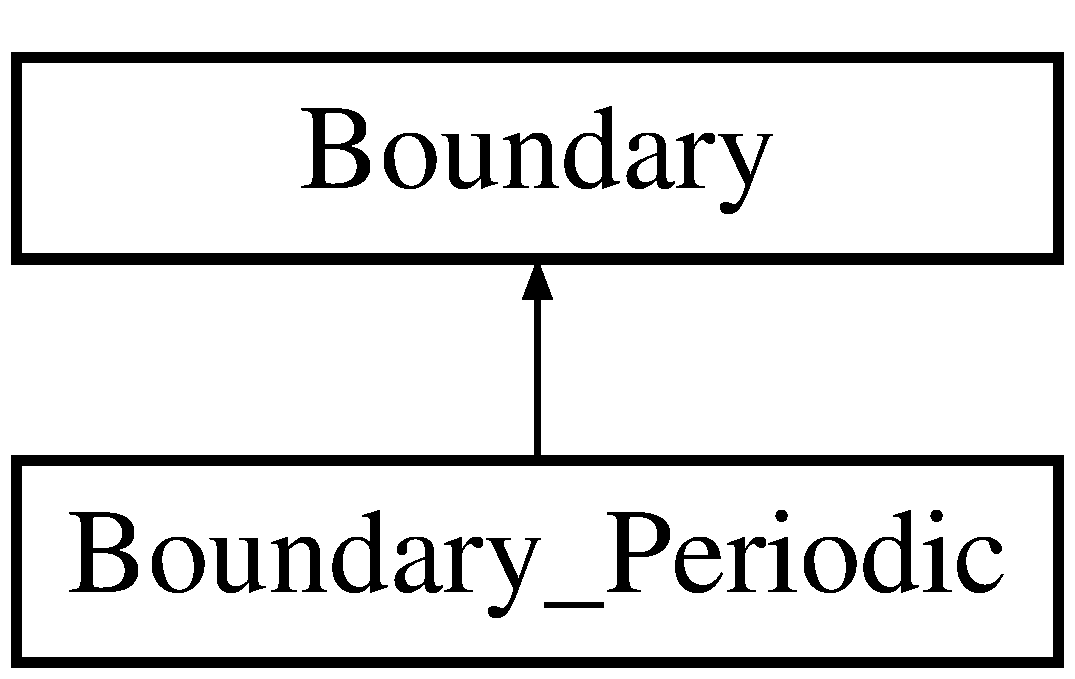
\includegraphics[height=2.000000cm]{class_boundary___periodic}
\end{center}
\end{figure}
\subsection*{Private Member Functions}
\begin{DoxyCompactItemize}
\item 
void \hyperlink{class_boundary___periodic_a72f5a45c04233e1c572098769f12fe82}{operator()} (\hyperlink{class_grid}{Grid} $\ast$g) const 
\end{DoxyCompactItemize}
\subsection*{Additional Inherited Members}


\subsection{Detailed Description}
Class for the computation of boundary fluxes for a periodic boundary condition. 

\subsection{Member Function Documentation}
\index{Boundary\+\_\+\+Periodic@{Boundary\+\_\+\+Periodic}!operator()@{operator()}}
\index{operator()@{operator()}!Boundary\+\_\+\+Periodic@{Boundary\+\_\+\+Periodic}}
\subsubsection[{\texorpdfstring{operator()(\+Grid $\ast$g) const }{operator()(Grid *g) const }}]{\setlength{\rightskip}{0pt plus 5cm}void Boundary\+\_\+\+Periodic\+::operator() (
\begin{DoxyParamCaption}
\item[{{\bf Grid} $\ast$}]{g}
\end{DoxyParamCaption}
) const\hspace{0.3cm}{\ttfamily [inline]}, {\ttfamily [private]}, {\ttfamily [virtual]}}\hypertarget{class_boundary___periodic_a72f5a45c04233e1c572098769f12fe82}{}\label{class_boundary___periodic_a72f5a45c04233e1c572098769f12fe82}
Operator that computes the boundary fluxes 
\begin{DoxyParams}{Parameters}
{\em g} & Pointer to grid object \\
\hline
\end{DoxyParams}


Implements \hyperlink{class_boundary_acbf1dee42af06301b014e50dbb76aa0c}{Boundary}.



The documentation for this class was generated from the following file\+:\begin{DoxyCompactItemize}
\item 
/home/doberle/\+Advanced C\+F\+D/acfd/\+Code/\hyperlink{boundary__periodic_8h}{boundary\+\_\+periodic.\+h}\end{DoxyCompactItemize}

\hypertarget{class_control}{}\section{Control Class Reference}
\label{class_control}\index{Control@{Control}}


Map that holds the contents of a control file.  




{\ttfamily \#include $<$control.\+h$>$}

\subsection*{Classes}
\begin{DoxyCompactItemize}
\item 
struct \hyperlink{struct_control_1_1_control_pair}{Control\+Pair}
\end{DoxyCompactItemize}
\subsection*{Public Member Functions}
\begin{DoxyCompactItemize}
\item 
\hyperlink{class_control_aa730aeda4517f40bc48ba1e46ebded77}{Control} ()
\item 
\hyperlink{class_control_a38ef2c3af6c8ed025fe1e32eaecde245}{Control} (string ctrl\+File)
\item 
\hyperlink{class_control_aedda1328c4f8b8d49bca8f0812d3bfd1}{$\sim$\+Control} ()
\item 
void \hyperlink{class_control_afeadb02134927ebd335d2ded31a080bc}{read} ()
\item 
bool \hyperlink{class_control_a25a6868383ae1da8c2dcfc9e1c08c9b7}{exists} (string key)
\item 
int \hyperlink{class_control_a1ab6db178c602c6a5d5f5b48edc01f61}{get\+Int} (string key, int tok=0)
\item 
bool \hyperlink{class_control_a50d1f887dd09e6292e4e07360be79824}{get\+Bool} (string key, int tok=0)
\item 
double \hyperlink{class_control_aacf80fb72e8d797d1b5396634e41ddc4}{get\+Double} (string key, int tok=0)
\item 
string \hyperlink{class_control_afdb5c4d692d258d9ba3b1a3596e10a4f}{get\+String} (string key, int tok=0)
\end{DoxyCompactItemize}
\subsection*{Static Public Member Functions}
\begin{DoxyCompactItemize}
\item 
static void \hyperlink{class_control_ac81ea08780126671aa88b90654f8a4fa}{find\+Key} (istream \&istr, string key)
\item 
static bool \hyperlink{class_control_ab2c73097c22b0f2693e5c86ff01d2775}{open\+File} (ifstream \&file, string name, string key)
\item 
static double \hyperlink{class_control_a22c3e26d6a7e40451a72ed6f25b45728}{read\+With\+Unit} (const char $\ast$timestr)
\end{DoxyCompactItemize}
\subsection*{Protected Member Functions}
\begin{DoxyCompactItemize}
\item 
void \hyperlink{class_control_a01104c38f1b71090108a52dcf0b3d1d8}{add\+Entry} (string key, string val, void $\ast$ptr=N\+U\+LL)
\item 
void \hyperlink{class_control_ab2764922690cecd881f3ac9c1e0ba8d6}{add\+Pointer} (string key, void $\ast$ptr, string val=\char`\"{}\char`\"{})
\item 
string \hyperlink{class_control_a194c1ebfe1f3774f2fc966b2c9d240b6}{get\+Token} (string key, int tok=0)
\end{DoxyCompactItemize}
\subsection*{Protected Attributes}
\begin{DoxyCompactItemize}
\item 
map$<$ string, \hyperlink{struct_control_1_1_control_pair}{Control\+Pair} $>$ \hyperlink{class_control_a95f5fb38688937d485753cb4d67b4099}{\+\_\+ctrl}
\item 
string \hyperlink{class_control_a9eb8605f3cba35efc0b6b76d38e9fd25}{\+\_\+file}
\end{DoxyCompactItemize}


\subsection{Detailed Description}
Map that holds the contents of a control file. 

In its present form, the control class is a simple map that holds the contents of the control file. The contents can be accessed as bools, integers, doubles or strings with string keys that are identical to the original keywords used in the file.

In addition to storing the control file data the control class allocates already all strategies used in the simulation. This follows an earlier design decision which was to separate the strategy from the rest of the simulation code\+: new strategies are easily implemented at a single place (this file here) and can be readily used anywhere without headaches of passing it down. Strategies can be accessed as void$\ast$ via the get\+Pointer(key) method. The void$\ast$ requires a correct cast at the time of use.

A single control object is then passed to the simulator upon construction and stored there. Hence, it is virtually accessible anywhere in the simulator. While the access time of a map (via string keys) is efficient, most receiving objects will still make local copies of the data to member variables, unless a data is used only infrequent, in which case it does not need to have a class analogy in form of a member variable.

Summary\+:
\begin{DoxyItemize}
\item control object provides original control file data virtually anywhere in the code
\item access with string keys that are the same as used in the control file
\item no hassle with passing down meter long interface lists
\item easy addition of new parameters
\item control class much shorter now, virtually no class variables (only a map)
\item control class can be re-\/read any time via \hyperlink{class_control_afeadb02134927ebd335d2ded31a080bc}{read()}, i.\+e., monitor changes
\item stand alone strategy allocation;
\item elegant grouping of strategy possible (e.\+g., factory together with output)
\item note\+: be careful with the right type casts with get\+Pointer() 
\end{DoxyItemize}

\subsection{Constructor \& Destructor Documentation}
\index{Control@{Control}!Control@{Control}}
\index{Control@{Control}!Control@{Control}}
\subsubsection[{\texorpdfstring{Control()}{Control()}}]{\setlength{\rightskip}{0pt plus 5cm}Control\+::\+Control (
\begin{DoxyParamCaption}
{}
\end{DoxyParamCaption}
)}\hypertarget{class_control_aa730aeda4517f40bc48ba1e46ebded77}{}\label{class_control_aa730aeda4517f40bc48ba1e46ebded77}
\index{Control@{Control}!Control@{Control}}
\index{Control@{Control}!Control@{Control}}
\subsubsection[{\texorpdfstring{Control(string ctrl\+File)}{Control(string ctrlFile)}}]{\setlength{\rightskip}{0pt plus 5cm}Control\+::\+Control (
\begin{DoxyParamCaption}
\item[{string}]{file}
\end{DoxyParamCaption}
)}\hypertarget{class_control_a38ef2c3af6c8ed025fe1e32eaecde245}{}\label{class_control_a38ef2c3af6c8ed025fe1e32eaecde245}
Constructor\+: control object from filename \index{Control@{Control}!````~Control@{$\sim$\+Control}}
\index{````~Control@{$\sim$\+Control}!Control@{Control}}
\subsubsection[{\texorpdfstring{$\sim$\+Control()}{~Control()}}]{\setlength{\rightskip}{0pt plus 5cm}Control\+::$\sim$\+Control (
\begin{DoxyParamCaption}
{}
\end{DoxyParamCaption}
)}\hypertarget{class_control_aedda1328c4f8b8d49bca8f0812d3bfd1}{}\label{class_control_aedda1328c4f8b8d49bca8f0812d3bfd1}
Destructor\+: loop over all map entries and delete pointers 

\subsection{Member Function Documentation}
\index{Control@{Control}!add\+Entry@{add\+Entry}}
\index{add\+Entry@{add\+Entry}!Control@{Control}}
\subsubsection[{\texorpdfstring{add\+Entry(string key, string val, void $\ast$ptr=\+N\+U\+L\+L)}{addEntry(string key, string val, void *ptr=NULL)}}]{\setlength{\rightskip}{0pt plus 5cm}void Control\+::add\+Entry (
\begin{DoxyParamCaption}
\item[{string}]{key, }
\item[{string}]{val, }
\item[{void $\ast$}]{ptr = {\ttfamily NULL}}
\end{DoxyParamCaption}
)\hspace{0.3cm}{\ttfamily [protected]}}\hypertarget{class_control_a01104c38f1b71090108a52dcf0b3d1d8}{}\label{class_control_a01104c38f1b71090108a52dcf0b3d1d8}
add a new entry to the map pass by value on purpose (so string constants can be used directly) a val == \char`\"{}default\char`\"{} leaves a field key unassigned \index{Control@{Control}!add\+Pointer@{add\+Pointer}}
\index{add\+Pointer@{add\+Pointer}!Control@{Control}}
\subsubsection[{\texorpdfstring{add\+Pointer(string key, void $\ast$ptr, string val="""")}{addPointer(string key, void *ptr, string val="")}}]{\setlength{\rightskip}{0pt plus 5cm}void Control\+::add\+Pointer (
\begin{DoxyParamCaption}
\item[{string}]{key, }
\item[{void $\ast$}]{ptr, }
\item[{string}]{val = {\ttfamily \char`\"{}\char`\"{}}}
\end{DoxyParamCaption}
)\hspace{0.3cm}{\ttfamily [protected]}}\hypertarget{class_control_ab2764922690cecd881f3ac9c1e0ba8d6}{}\label{class_control_ab2764922690cecd881f3ac9c1e0ba8d6}
add a pointer to the map, create entries on the fly pass by value on purpose (so string constants can be used directly) \index{Control@{Control}!exists@{exists}}
\index{exists@{exists}!Control@{Control}}
\subsubsection[{\texorpdfstring{exists(string key)}{exists(string key)}}]{\setlength{\rightskip}{0pt plus 5cm}bool Control\+::exists (
\begin{DoxyParamCaption}
\item[{string}]{key}
\end{DoxyParamCaption}
)}\hypertarget{class_control_a25a6868383ae1da8c2dcfc9e1c08c9b7}{}\label{class_control_a25a6868383ae1da8c2dcfc9e1c08c9b7}
see if a keyword is in the control file 
\begin{DoxyParams}{Parameters}
{\em key} & keyword as it appears in the control file \\
\hline
\end{DoxyParams}
\index{Control@{Control}!find\+Key@{find\+Key}}
\index{find\+Key@{find\+Key}!Control@{Control}}
\subsubsection[{\texorpdfstring{find\+Key(istream \&istr, string key)}{findKey(istream &istr, string key)}}]{\setlength{\rightskip}{0pt plus 5cm}void Control\+::find\+Key (
\begin{DoxyParamCaption}
\item[{istream \&}]{istr, }
\item[{string}]{key}
\end{DoxyParamCaption}
)\hspace{0.3cm}{\ttfamily [static]}}\hypertarget{class_control_ac81ea08780126671aa88b90654f8a4fa}{}\label{class_control_ac81ea08780126671aa88b90654f8a4fa}
read lines in a stream until the key string is found (at the beginning of a line) 
\begin{DoxyParams}{Parameters}
{\em istr} & the stream to be read from \\
\hline
{\em key} & the key we are looking for \\
\hline
\end{DoxyParams}
\index{Control@{Control}!get\+Bool@{get\+Bool}}
\index{get\+Bool@{get\+Bool}!Control@{Control}}
\subsubsection[{\texorpdfstring{get\+Bool(string key, int tok=0)}{getBool(string key, int tok=0)}}]{\setlength{\rightskip}{0pt plus 5cm}bool Control\+::get\+Bool (
\begin{DoxyParamCaption}
\item[{string}]{key, }
\item[{int}]{tok = {\ttfamily 0}}
\end{DoxyParamCaption}
)}\hypertarget{class_control_a50d1f887dd09e6292e4e07360be79824}{}\label{class_control_a50d1f887dd09e6292e4e07360be79824}
return the control parameter as bool if key is not in map, false will be returned 
\begin{DoxyParams}{Parameters}
{\em key} & keyword as it appears in the control file \\
\hline
{\em tok} & if tok$>$ 0\+: read the tokth token \\
\hline
\end{DoxyParams}
\index{Control@{Control}!get\+Double@{get\+Double}}
\index{get\+Double@{get\+Double}!Control@{Control}}
\subsubsection[{\texorpdfstring{get\+Double(string key, int tok=0)}{getDouble(string key, int tok=0)}}]{\setlength{\rightskip}{0pt plus 5cm}double Control\+::get\+Double (
\begin{DoxyParamCaption}
\item[{string}]{key, }
\item[{int}]{tok = {\ttfamily 0}}
\end{DoxyParamCaption}
)}\hypertarget{class_control_aacf80fb72e8d797d1b5396634e41ddc4}{}\label{class_control_aacf80fb72e8d797d1b5396634e41ddc4}
return the control parameter as double a unit following the number will be considered if key is not in map, \char`\"{}-\/1\char`\"{} will be returned 
\begin{DoxyParams}{Parameters}
{\em key} & keyword as it appears in the control file \\
\hline
{\em tok} & if tok$>$ 0\+: read the tokth token \\
\hline
\end{DoxyParams}
\index{Control@{Control}!get\+Int@{get\+Int}}
\index{get\+Int@{get\+Int}!Control@{Control}}
\subsubsection[{\texorpdfstring{get\+Int(string key, int tok=0)}{getInt(string key, int tok=0)}}]{\setlength{\rightskip}{0pt plus 5cm}int Control\+::get\+Int (
\begin{DoxyParamCaption}
\item[{string}]{key, }
\item[{int}]{tok = {\ttfamily 0}}
\end{DoxyParamCaption}
)}\hypertarget{class_control_a1ab6db178c602c6a5d5f5b48edc01f61}{}\label{class_control_a1ab6db178c602c6a5d5f5b48edc01f61}
return the control parameter as integer if key is not in map, -\/1 will be returned 
\begin{DoxyParams}{Parameters}
{\em key} & keyword as it appears in the control file \\
\hline
{\em tok} & if tok$>$ 0\+: read the tokth token \\
\hline
\end{DoxyParams}
\index{Control@{Control}!get\+String@{get\+String}}
\index{get\+String@{get\+String}!Control@{Control}}
\subsubsection[{\texorpdfstring{get\+String(string key, int tok=0)}{getString(string key, int tok=0)}}]{\setlength{\rightskip}{0pt plus 5cm}string Control\+::get\+String (
\begin{DoxyParamCaption}
\item[{string}]{key, }
\item[{int}]{tok = {\ttfamily 0}}
\end{DoxyParamCaption}
)}\hypertarget{class_control_afdb5c4d692d258d9ba3b1a3596e10a4f}{}\label{class_control_afdb5c4d692d258d9ba3b1a3596e10a4f}
return the control parameter as string if key is not in map, \char`\"{}default\char`\"{} will be returned 
\begin{DoxyParams}{Parameters}
{\em key} & keyword as it appears in the control file \\
\hline
{\em tok} & if tok$>$ 0\+: read the tokth token \\
\hline
\end{DoxyParams}
\index{Control@{Control}!get\+Token@{get\+Token}}
\index{get\+Token@{get\+Token}!Control@{Control}}
\subsubsection[{\texorpdfstring{get\+Token(string key, int tok=0)}{getToken(string key, int tok=0)}}]{\setlength{\rightskip}{0pt plus 5cm}string Control\+::get\+Token (
\begin{DoxyParamCaption}
\item[{string}]{key, }
\item[{int}]{tok = {\ttfamily 0}}
\end{DoxyParamCaption}
)\hspace{0.3cm}{\ttfamily [protected]}}\hypertarget{class_control_a194c1ebfe1f3774f2fc966b2c9d240b6}{}\label{class_control_a194c1ebfe1f3774f2fc966b2c9d240b6}
returns a token from an item \index{Control@{Control}!open\+File@{open\+File}}
\index{open\+File@{open\+File}!Control@{Control}}
\subsubsection[{\texorpdfstring{open\+File(ifstream \&file, string name, string key)}{openFile(ifstream &file, string name, string key)}}]{\setlength{\rightskip}{0pt plus 5cm}bool Control\+::open\+File (
\begin{DoxyParamCaption}
\item[{ifstream \&}]{file, }
\item[{string}]{name, }
\item[{string}]{key}
\end{DoxyParamCaption}
)\hspace{0.3cm}{\ttfamily [static]}}\hypertarget{class_control_ab2c73097c22b0f2693e5c86ff01d2775}{}\label{class_control_ab2c73097c22b0f2693e5c86ff01d2775}
attempts to open a the file with name and place it past the optional key (at the beginning of a line) 
\begin{DoxyParams}{Parameters}
{\em file} & the stream to be opened for reading \\
\hline
{\em name} & filepath and name \\
\hline
{\em key} & key to be found \\
\hline
\end{DoxyParams}
\index{Control@{Control}!read@{read}}
\index{read@{read}!Control@{Control}}
\subsubsection[{\texorpdfstring{read()}{read()}}]{\setlength{\rightskip}{0pt plus 5cm}void Control\+::read (
\begin{DoxyParamCaption}
{}
\end{DoxyParamCaption}
)}\hypertarget{class_control_afeadb02134927ebd335d2ded31a080bc}{}\label{class_control_afeadb02134927ebd335d2ded31a080bc}
read the control file \index{Control@{Control}!read\+With\+Unit@{read\+With\+Unit}}
\index{read\+With\+Unit@{read\+With\+Unit}!Control@{Control}}
\subsubsection[{\texorpdfstring{read\+With\+Unit(const char $\ast$timestr)}{readWithUnit(const char *timestr)}}]{\setlength{\rightskip}{0pt plus 5cm}double Control\+::read\+With\+Unit (
\begin{DoxyParamCaption}
\item[{const char $\ast$}]{unitstr}
\end{DoxyParamCaption}
)\hspace{0.3cm}{\ttfamily [static]}}\hypertarget{class_control_a22c3e26d6a7e40451a72ed6f25b45728}{}\label{class_control_a22c3e26d6a7e40451a72ed6f25b45728}
reads a \char`\"{}number unit\char`\"{} string and converts it to a single double considering the unit returns -\/1 if nothing was converted 

\subsection{Member Data Documentation}
\index{Control@{Control}!\+\_\+ctrl@{\+\_\+ctrl}}
\index{\+\_\+ctrl@{\+\_\+ctrl}!Control@{Control}}
\subsubsection[{\texorpdfstring{\+\_\+ctrl}{_ctrl}}]{\setlength{\rightskip}{0pt plus 5cm}map$<$string,{\bf Control\+Pair}$>$ Control\+::\+\_\+ctrl\hspace{0.3cm}{\ttfamily [protected]}}\hypertarget{class_control_a95f5fb38688937d485753cb4d67b4099}{}\label{class_control_a95f5fb38688937d485753cb4d67b4099}
\index{Control@{Control}!\+\_\+file@{\+\_\+file}}
\index{\+\_\+file@{\+\_\+file}!Control@{Control}}
\subsubsection[{\texorpdfstring{\+\_\+file}{_file}}]{\setlength{\rightskip}{0pt plus 5cm}string Control\+::\+\_\+file\hspace{0.3cm}{\ttfamily [protected]}}\hypertarget{class_control_a9eb8605f3cba35efc0b6b76d38e9fd25}{}\label{class_control_a9eb8605f3cba35efc0b6b76d38e9fd25}


The documentation for this class was generated from the following files\+:\begin{DoxyCompactItemize}
\item 
/home/doberle/\+Advanced C\+F\+D/acfd/\+Code/\hyperlink{control_8h}{control.\+h}\item 
/home/doberle/\+Advanced C\+F\+D/acfd/\+Code/\hyperlink{control_8cpp}{control.\+cpp}\end{DoxyCompactItemize}

\hypertarget{struct_control_1_1_control_pair}{}\section{Control\+:\+:Control\+Pair Struct Reference}
\label{struct_control_1_1_control_pair}\index{Control\+::\+Control\+Pair@{Control\+::\+Control\+Pair}}


{\ttfamily \#include $<$control.\+h$>$}

\subsection*{Public Attributes}
\begin{DoxyCompactItemize}
\item 
string \hyperlink{struct_control_1_1_control_pair_a361316ff538781a3ffecf101c2ca68e2}{\+\_\+val}
\item 
void $\ast$ \hyperlink{struct_control_1_1_control_pair_a3cb5abe162d7147180a4b932167ab110}{\+\_\+ptr}
\end{DoxyCompactItemize}


\subsection{Member Data Documentation}
\index{Control\+::\+Control\+Pair@{Control\+::\+Control\+Pair}!\+\_\+ptr@{\+\_\+ptr}}
\index{\+\_\+ptr@{\+\_\+ptr}!Control\+::\+Control\+Pair@{Control\+::\+Control\+Pair}}
\subsubsection[{\texorpdfstring{\+\_\+ptr}{_ptr}}]{\setlength{\rightskip}{0pt plus 5cm}void$\ast$ Control\+::\+Control\+Pair\+::\+\_\+ptr}\hypertarget{struct_control_1_1_control_pair_a3cb5abe162d7147180a4b932167ab110}{}\label{struct_control_1_1_control_pair_a3cb5abe162d7147180a4b932167ab110}
\index{Control\+::\+Control\+Pair@{Control\+::\+Control\+Pair}!\+\_\+val@{\+\_\+val}}
\index{\+\_\+val@{\+\_\+val}!Control\+::\+Control\+Pair@{Control\+::\+Control\+Pair}}
\subsubsection[{\texorpdfstring{\+\_\+val}{_val}}]{\setlength{\rightskip}{0pt plus 5cm}string Control\+::\+Control\+Pair\+::\+\_\+val}\hypertarget{struct_control_1_1_control_pair_a361316ff538781a3ffecf101c2ca68e2}{}\label{struct_control_1_1_control_pair_a361316ff538781a3ffecf101c2ca68e2}


The documentation for this struct was generated from the following file\+:\begin{DoxyCompactItemize}
\item 
/home/doberle/\+Advanced C\+F\+D/acfd/\+Code/\hyperlink{control_8h}{control.\+h}\end{DoxyCompactItemize}

\hypertarget{class_driver}{}\section{Driver Class Reference}
\label{class_driver}\index{Driver@{Driver}}


Abstract class for a simulation code driver.  




{\ttfamily \#include $<$driver.\+h$>$}

Inheritance diagram for Driver\+:\begin{figure}[H]
\begin{center}
\leavevmode
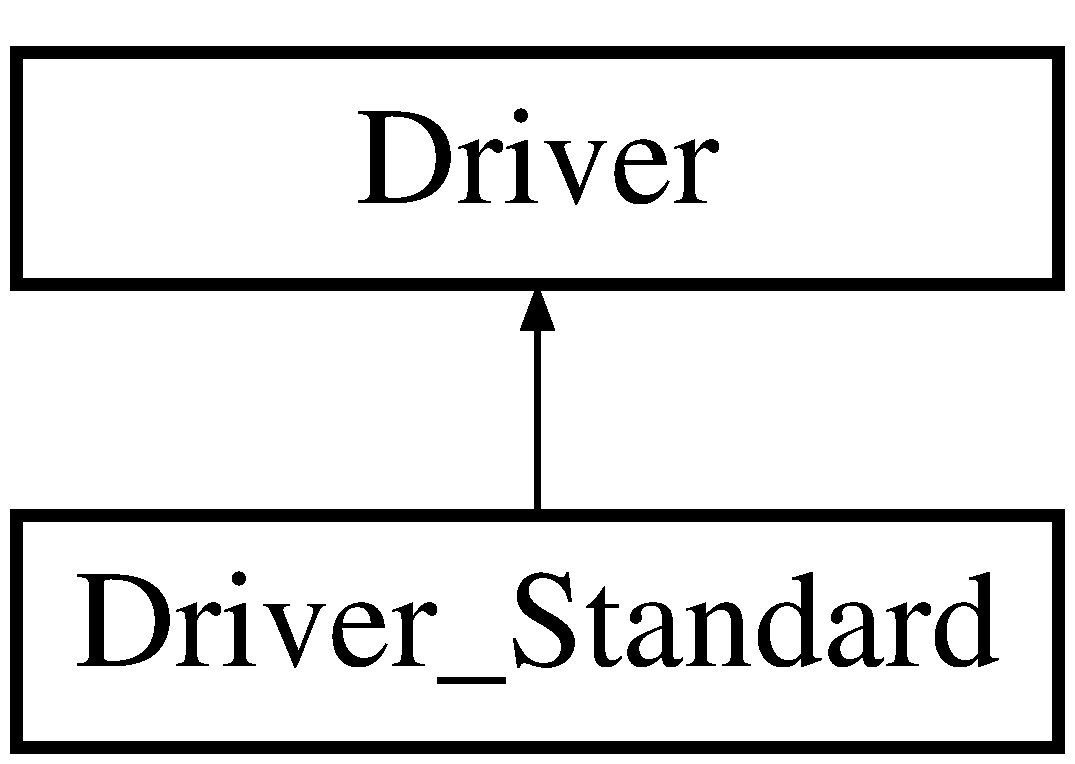
\includegraphics[height=2.000000cm]{class_driver}
\end{center}
\end{figure}
\subsection*{Public Member Functions}
\begin{DoxyCompactItemize}
\item 
virtual \hyperlink{class_driver_a2864fd05273f30e23aa959c92ef8a5b9}{$\sim$\+Driver} ()
\item 
virtual void \hyperlink{class_driver_a1cebfd199c4b9dac845235479e3b485b}{operator()} ()=0
\end{DoxyCompactItemize}


\subsection{Detailed Description}
Abstract class for a simulation code driver. 

\subsection{Constructor \& Destructor Documentation}
\index{Driver@{Driver}!````~Driver@{$\sim$\+Driver}}
\index{````~Driver@{$\sim$\+Driver}!Driver@{Driver}}
\subsubsection[{\texorpdfstring{$\sim$\+Driver()}{~Driver()}}]{\setlength{\rightskip}{0pt plus 5cm}virtual Driver\+::$\sim$\+Driver (
\begin{DoxyParamCaption}
{}
\end{DoxyParamCaption}
)\hspace{0.3cm}{\ttfamily [inline]}, {\ttfamily [virtual]}}\hypertarget{class_driver_a2864fd05273f30e23aa959c92ef8a5b9}{}\label{class_driver_a2864fd05273f30e23aa959c92ef8a5b9}


\subsection{Member Function Documentation}
\index{Driver@{Driver}!operator()@{operator()}}
\index{operator()@{operator()}!Driver@{Driver}}
\subsubsection[{\texorpdfstring{operator()()=0}{operator()()=0}}]{\setlength{\rightskip}{0pt plus 5cm}virtual void Driver\+::operator() (
\begin{DoxyParamCaption}
{}
\end{DoxyParamCaption}
)\hspace{0.3cm}{\ttfamily [pure virtual]}}\hypertarget{class_driver_a1cebfd199c4b9dac845235479e3b485b}{}\label{class_driver_a1cebfd199c4b9dac845235479e3b485b}
Run the simulation 

Implemented in \hyperlink{class_driver___standard_a5a3fda905d229fd530f8057262b4d44c}{Driver\+\_\+\+Standard}.



The documentation for this class was generated from the following file\+:\begin{DoxyCompactItemize}
\item 
/home/doberle/\+Advanced C\+F\+D/acfd/\+Code/\hyperlink{driver_8h}{driver.\+h}\end{DoxyCompactItemize}

\hypertarget{class_driver___standard}{}\section{Driver\+\_\+\+Standard Class Reference}
\label{class_driver___standard}\index{Driver\+\_\+\+Standard@{Driver\+\_\+\+Standard}}


\hyperlink{class_driver}{Driver} for numerical simulation of conservation laws.  




{\ttfamily \#include $<$driver\+\_\+standard.\+h$>$}

Inheritance diagram for Driver\+\_\+\+Standard\+:\begin{figure}[H]
\begin{center}
\leavevmode
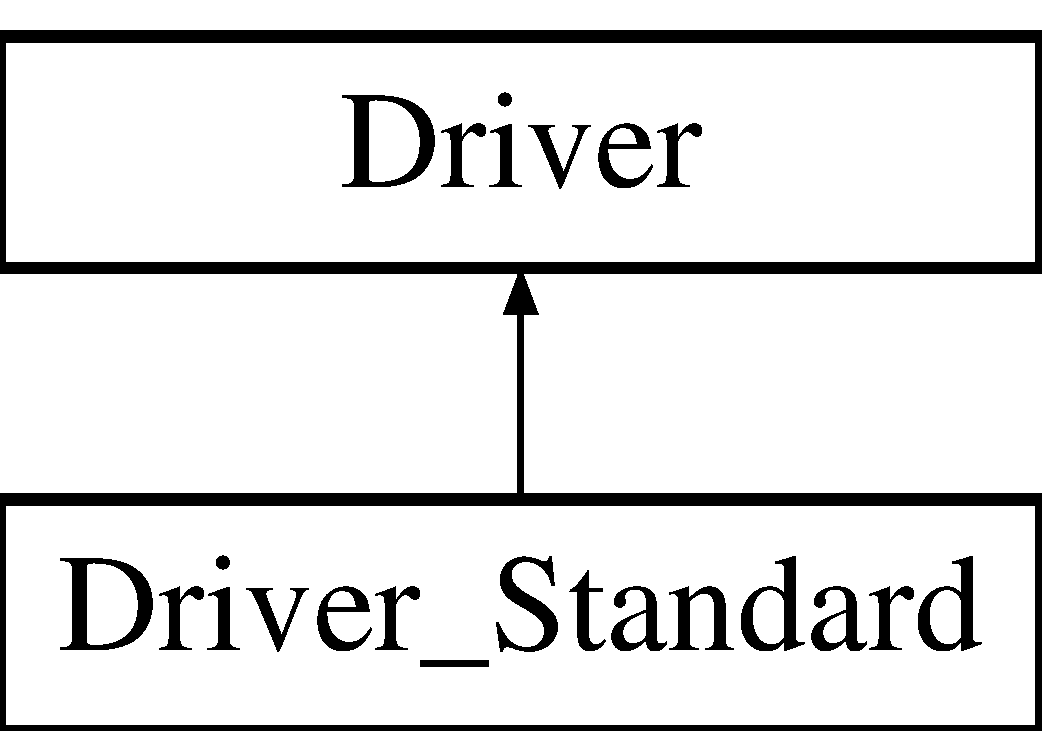
\includegraphics[height=2.000000cm]{class_driver___standard}
\end{center}
\end{figure}
\subsection*{Public Member Functions}
\begin{DoxyCompactItemize}
\item 
void \hyperlink{class_driver___standard_a5a3fda905d229fd530f8057262b4d44c}{operator()} ()
\end{DoxyCompactItemize}


\subsection{Detailed Description}
\hyperlink{class_driver}{Driver} for numerical simulation of conservation laws. 

\subsection{Member Function Documentation}
\index{Driver\+\_\+\+Standard@{Driver\+\_\+\+Standard}!operator()@{operator()}}
\index{operator()@{operator()}!Driver\+\_\+\+Standard@{Driver\+\_\+\+Standard}}
\subsubsection[{\texorpdfstring{operator()()}{operator()()}}]{\setlength{\rightskip}{0pt plus 5cm}void Driver\+\_\+\+Standard\+::operator() (
\begin{DoxyParamCaption}
{}
\end{DoxyParamCaption}
)\hspace{0.3cm}{\ttfamily [virtual]}}\hypertarget{class_driver___standard_a5a3fda905d229fd530f8057262b4d44c}{}\label{class_driver___standard_a5a3fda905d229fd530f8057262b4d44c}
Run the simulation 

Implements \hyperlink{class_driver_a1cebfd199c4b9dac845235479e3b485b}{Driver}.



The documentation for this class was generated from the following files\+:\begin{DoxyCompactItemize}
\item 
/home/doberle/\+Advanced C\+F\+D/acfd/\+Code/\hyperlink{driver__standard_8h}{driver\+\_\+standard.\+h}\item 
/home/doberle/\+Advanced C\+F\+D/acfd/\+Code/\hyperlink{driver__standard_8cpp}{driver\+\_\+standard.\+cpp}\end{DoxyCompactItemize}

\hypertarget{class_fluxes}{}\section{Fluxes Class Reference}
\label{class_fluxes}\index{Fluxes@{Fluxes}}


Class for the computation of numerical fluxes over cell interfaces for a given conservation law.  




{\ttfamily \#include $<$fluxes.\+h$>$}

Inheritance diagram for Fluxes\+:\begin{figure}[H]
\begin{center}
\leavevmode
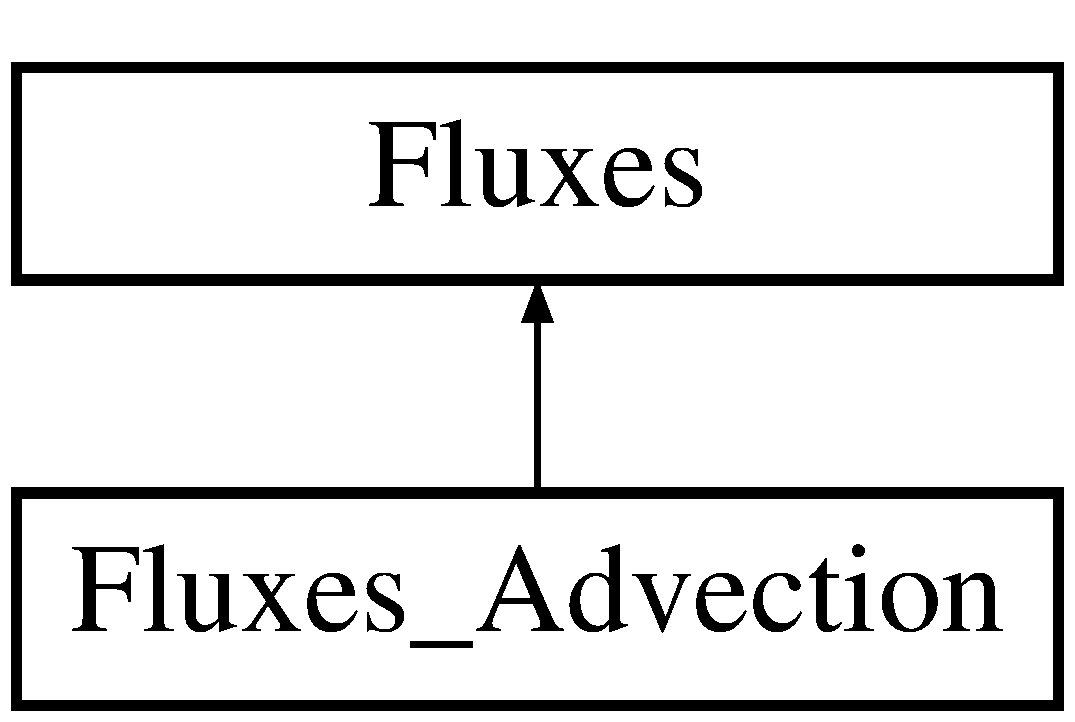
\includegraphics[height=2.000000cm]{class_fluxes}
\end{center}
\end{figure}
\subsection*{Public Member Functions}
\begin{DoxyCompactItemize}
\item 
\hyperlink{class_fluxes_accfbcaf73689eb08bee2b799cc981dcf}{Fluxes} (\hyperlink{class_control}{Control} $\ast$c, \hyperlink{class_grid}{Grid} $\ast$g)
\item 
virtual \hyperlink{class_fluxes_a18143f941adeeaf901f39e10b0c7a8f7}{$\sim$\+Fluxes} ()
\item 
virtual void \hyperlink{class_fluxes_ad3c2d7326f428cf6543e5ef374aa1b90}{operator()} (\hyperlink{class_grid}{Grid} $\ast$g) const =0
\end{DoxyCompactItemize}
\subsection*{Protected Member Functions}
\begin{DoxyCompactItemize}
\item 
void \hyperlink{class_fluxes_aed960cd3e402e665449ffccd33f448d1}{reinitialize\+\_\+fluxes} (\hyperlink{class_grid}{Grid} $\ast$g) const 
\item 
double \hyperlink{class_fluxes_ae159dd9fd9431e6ddcdeef7d04090a9f}{minmod} (double a, double b) const 
\end{DoxyCompactItemize}
\subsection*{Protected Attributes}
\begin{DoxyCompactItemize}
\item 
\hyperlink{class_control}{Control} $\ast$ \hyperlink{class_fluxes_a82e80aa9b4d9431508850c1fe1d91c56}{\+\_\+c}
\end{DoxyCompactItemize}


\subsection{Detailed Description}
Class for the computation of numerical fluxes over cell interfaces for a given conservation law. 

\subsection{Constructor \& Destructor Documentation}
\index{Fluxes@{Fluxes}!Fluxes@{Fluxes}}
\index{Fluxes@{Fluxes}!Fluxes@{Fluxes}}
\subsubsection[{\texorpdfstring{Fluxes(\+Control $\ast$c, Grid $\ast$g)}{Fluxes(Control *c, Grid *g)}}]{\setlength{\rightskip}{0pt plus 5cm}Fluxes\+::\+Fluxes (
\begin{DoxyParamCaption}
\item[{{\bf Control} $\ast$}]{c, }
\item[{{\bf Grid} $\ast$}]{g}
\end{DoxyParamCaption}
)}\hypertarget{class_fluxes_accfbcaf73689eb08bee2b799cc981dcf}{}\label{class_fluxes_accfbcaf73689eb08bee2b799cc981dcf}
Construct from \hyperlink{class_control}{Control} and \hyperlink{class_grid}{Grid} objects \index{Fluxes@{Fluxes}!````~Fluxes@{$\sim$\+Fluxes}}
\index{````~Fluxes@{$\sim$\+Fluxes}!Fluxes@{Fluxes}}
\subsubsection[{\texorpdfstring{$\sim$\+Fluxes()}{~Fluxes()}}]{\setlength{\rightskip}{0pt plus 5cm}virtual Fluxes\+::$\sim$\+Fluxes (
\begin{DoxyParamCaption}
{}
\end{DoxyParamCaption}
)\hspace{0.3cm}{\ttfamily [inline]}, {\ttfamily [virtual]}}\hypertarget{class_fluxes_a18143f941adeeaf901f39e10b0c7a8f7}{}\label{class_fluxes_a18143f941adeeaf901f39e10b0c7a8f7}


\subsection{Member Function Documentation}
\index{Fluxes@{Fluxes}!minmod@{minmod}}
\index{minmod@{minmod}!Fluxes@{Fluxes}}
\subsubsection[{\texorpdfstring{minmod(double a, double b) const }{minmod(double a, double b) const }}]{\setlength{\rightskip}{0pt plus 5cm}double Fluxes\+::minmod (
\begin{DoxyParamCaption}
\item[{double}]{a, }
\item[{double}]{b}
\end{DoxyParamCaption}
) const\hspace{0.3cm}{\ttfamily [inline]}, {\ttfamily [protected]}}\hypertarget{class_fluxes_ae159dd9fd9431e6ddcdeef7d04090a9f}{}\label{class_fluxes_ae159dd9fd9431e6ddcdeef7d04090a9f}
Minmod of two numbers \index{Fluxes@{Fluxes}!operator()@{operator()}}
\index{operator()@{operator()}!Fluxes@{Fluxes}}
\subsubsection[{\texorpdfstring{operator()(\+Grid $\ast$g) const =0}{operator()(Grid *g) const =0}}]{\setlength{\rightskip}{0pt plus 5cm}virtual void Fluxes\+::operator() (
\begin{DoxyParamCaption}
\item[{{\bf Grid} $\ast$}]{g}
\end{DoxyParamCaption}
) const\hspace{0.3cm}{\ttfamily [pure virtual]}}\hypertarget{class_fluxes_ad3c2d7326f428cf6543e5ef374aa1b90}{}\label{class_fluxes_ad3c2d7326f428cf6543e5ef374aa1b90}
Compute fluxes based on a scheme given in the control file 

Implemented in \hyperlink{class_fluxes___advection_a3e464c726fac986b627af81975b2ad68}{Fluxes\+\_\+\+Advection}.

\index{Fluxes@{Fluxes}!reinitialize\+\_\+fluxes@{reinitialize\+\_\+fluxes}}
\index{reinitialize\+\_\+fluxes@{reinitialize\+\_\+fluxes}!Fluxes@{Fluxes}}
\subsubsection[{\texorpdfstring{reinitialize\+\_\+fluxes(\+Grid $\ast$g) const }{reinitialize_fluxes(Grid *g) const }}]{\setlength{\rightskip}{0pt plus 5cm}void Fluxes\+::reinitialize\+\_\+fluxes (
\begin{DoxyParamCaption}
\item[{{\bf Grid} $\ast$}]{g}
\end{DoxyParamCaption}
) const\hspace{0.3cm}{\ttfamily [protected]}}\hypertarget{class_fluxes_aed960cd3e402e665449ffccd33f448d1}{}\label{class_fluxes_aed960cd3e402e665449ffccd33f448d1}
Set all fluxes to zero 

\subsection{Member Data Documentation}
\index{Fluxes@{Fluxes}!\+\_\+c@{\+\_\+c}}
\index{\+\_\+c@{\+\_\+c}!Fluxes@{Fluxes}}
\subsubsection[{\texorpdfstring{\+\_\+c}{_c}}]{\setlength{\rightskip}{0pt plus 5cm}{\bf Control}$\ast$ Fluxes\+::\+\_\+c\hspace{0.3cm}{\ttfamily [protected]}}\hypertarget{class_fluxes_a82e80aa9b4d9431508850c1fe1d91c56}{}\label{class_fluxes_a82e80aa9b4d9431508850c1fe1d91c56}


The documentation for this class was generated from the following files\+:\begin{DoxyCompactItemize}
\item 
/home/doberle/\+Advanced C\+F\+D/acfd/\+Code/\hyperlink{fluxes_8h}{fluxes.\+h}\item 
/home/doberle/\+Advanced C\+F\+D/acfd/\+Code/\hyperlink{fluxes_8cpp}{fluxes.\+cpp}\end{DoxyCompactItemize}

\hypertarget{class_fluxes___advection}{}\section{Fluxes\+\_\+\+Advection Class Reference}
\label{class_fluxes___advection}\index{Fluxes\+\_\+\+Advection@{Fluxes\+\_\+\+Advection}}


Computation of fluxes for the linear advection-\/diffusion equation.  




{\ttfamily \#include $<$fluxes\+\_\+advection.\+h$>$}

Inheritance diagram for Fluxes\+\_\+\+Advection\+:\begin{figure}[H]
\begin{center}
\leavevmode
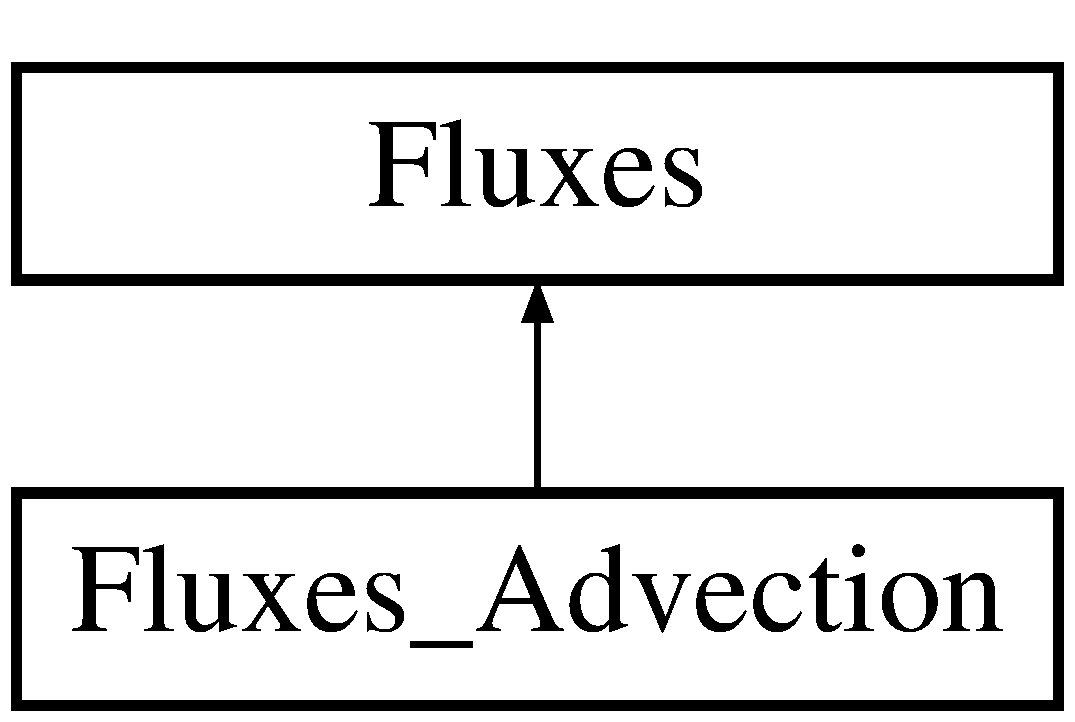
\includegraphics[height=2.000000cm]{class_fluxes___advection}
\end{center}
\end{figure}
\subsection*{Public Member Functions}
\begin{DoxyCompactItemize}
\item 
\hyperlink{class_fluxes___advection_a24b69e1dba304f7267df903d9475c3d3}{Fluxes\+\_\+\+Advection} (\hyperlink{class_control}{Control} $\ast$c, \hyperlink{class_grid}{Grid} $\ast$g)
\item 
\hyperlink{class_fluxes___advection_a4fcf0d50fb99dbe44b0718a9065e2618}{$\sim$\+Fluxes\+\_\+\+Advection} ()
\item 
void \hyperlink{class_fluxes___advection_a3e464c726fac986b627af81975b2ad68}{operator()} (\hyperlink{class_grid}{Grid} $\ast$g) const 
\end{DoxyCompactItemize}
\subsection*{Private Member Functions}
\begin{DoxyCompactItemize}
\item 
void \hyperlink{class_fluxes___advection_aaf2de2525ef3dcafe15afd814fa2f4be}{fluxes\+\_\+conv\+\_\+central} (\hyperlink{class_grid}{Grid} $\ast$g) const 
\item 
void \hyperlink{class_fluxes___advection_a4f6e8629d5120b16763aa07b5189b38b}{fluxes\+\_\+conv\+\_\+upwind} (\hyperlink{class_grid}{Grid} $\ast$g) const 
\end{DoxyCompactItemize}
\subsection*{Additional Inherited Members}


\subsection{Detailed Description}
Computation of fluxes for the linear advection-\/diffusion equation. 

\subsection{Constructor \& Destructor Documentation}
\index{Fluxes\+\_\+\+Advection@{Fluxes\+\_\+\+Advection}!Fluxes\+\_\+\+Advection@{Fluxes\+\_\+\+Advection}}
\index{Fluxes\+\_\+\+Advection@{Fluxes\+\_\+\+Advection}!Fluxes\+\_\+\+Advection@{Fluxes\+\_\+\+Advection}}
\subsubsection[{\texorpdfstring{Fluxes\+\_\+\+Advection(\+Control $\ast$c, Grid $\ast$g)}{Fluxes_Advection(Control *c, Grid *g)}}]{\setlength{\rightskip}{0pt plus 5cm}Fluxes\+\_\+\+Advection\+::\+Fluxes\+\_\+\+Advection (
\begin{DoxyParamCaption}
\item[{{\bf Control} $\ast$}]{c, }
\item[{{\bf Grid} $\ast$}]{g}
\end{DoxyParamCaption}
)}\hypertarget{class_fluxes___advection_a24b69e1dba304f7267df903d9475c3d3}{}\label{class_fluxes___advection_a24b69e1dba304f7267df903d9475c3d3}
\index{Fluxes\+\_\+\+Advection@{Fluxes\+\_\+\+Advection}!````~Fluxes\+\_\+\+Advection@{$\sim$\+Fluxes\+\_\+\+Advection}}
\index{````~Fluxes\+\_\+\+Advection@{$\sim$\+Fluxes\+\_\+\+Advection}!Fluxes\+\_\+\+Advection@{Fluxes\+\_\+\+Advection}}
\subsubsection[{\texorpdfstring{$\sim$\+Fluxes\+\_\+\+Advection()}{~Fluxes_Advection()}}]{\setlength{\rightskip}{0pt plus 5cm}Fluxes\+\_\+\+Advection\+::$\sim$\+Fluxes\+\_\+\+Advection (
\begin{DoxyParamCaption}
{}
\end{DoxyParamCaption}
)\hspace{0.3cm}{\ttfamily [inline]}}\hypertarget{class_fluxes___advection_a4fcf0d50fb99dbe44b0718a9065e2618}{}\label{class_fluxes___advection_a4fcf0d50fb99dbe44b0718a9065e2618}


\subsection{Member Function Documentation}
\index{Fluxes\+\_\+\+Advection@{Fluxes\+\_\+\+Advection}!fluxes\+\_\+conv\+\_\+central@{fluxes\+\_\+conv\+\_\+central}}
\index{fluxes\+\_\+conv\+\_\+central@{fluxes\+\_\+conv\+\_\+central}!Fluxes\+\_\+\+Advection@{Fluxes\+\_\+\+Advection}}
\subsubsection[{\texorpdfstring{fluxes\+\_\+conv\+\_\+central(\+Grid $\ast$g) const }{fluxes_conv_central(Grid *g) const }}]{\setlength{\rightskip}{0pt plus 5cm}void Fluxes\+\_\+\+Advection\+::fluxes\+\_\+conv\+\_\+central (
\begin{DoxyParamCaption}
\item[{{\bf Grid} $\ast$}]{g}
\end{DoxyParamCaption}
) const\hspace{0.3cm}{\ttfamily [private]}}\hypertarget{class_fluxes___advection_aaf2de2525ef3dcafe15afd814fa2f4be}{}\label{class_fluxes___advection_aaf2de2525ef3dcafe15afd814fa2f4be}
Central scheme for the advection term \index{Fluxes\+\_\+\+Advection@{Fluxes\+\_\+\+Advection}!fluxes\+\_\+conv\+\_\+upwind@{fluxes\+\_\+conv\+\_\+upwind}}
\index{fluxes\+\_\+conv\+\_\+upwind@{fluxes\+\_\+conv\+\_\+upwind}!Fluxes\+\_\+\+Advection@{Fluxes\+\_\+\+Advection}}
\subsubsection[{\texorpdfstring{fluxes\+\_\+conv\+\_\+upwind(\+Grid $\ast$g) const }{fluxes_conv_upwind(Grid *g) const }}]{\setlength{\rightskip}{0pt plus 5cm}void Fluxes\+\_\+\+Advection\+::fluxes\+\_\+conv\+\_\+upwind (
\begin{DoxyParamCaption}
\item[{{\bf Grid} $\ast$}]{g}
\end{DoxyParamCaption}
) const\hspace{0.3cm}{\ttfamily [private]}}\hypertarget{class_fluxes___advection_a4f6e8629d5120b16763aa07b5189b38b}{}\label{class_fluxes___advection_a4f6e8629d5120b16763aa07b5189b38b}
Upwind scheme for the advection term \index{Fluxes\+\_\+\+Advection@{Fluxes\+\_\+\+Advection}!operator()@{operator()}}
\index{operator()@{operator()}!Fluxes\+\_\+\+Advection@{Fluxes\+\_\+\+Advection}}
\subsubsection[{\texorpdfstring{operator()(\+Grid $\ast$g) const }{operator()(Grid *g) const }}]{\setlength{\rightskip}{0pt plus 5cm}void Fluxes\+\_\+\+Advection\+::operator() (
\begin{DoxyParamCaption}
\item[{{\bf Grid} $\ast$}]{g}
\end{DoxyParamCaption}
) const\hspace{0.3cm}{\ttfamily [inline]}, {\ttfamily [virtual]}}\hypertarget{class_fluxes___advection_a3e464c726fac986b627af81975b2ad68}{}\label{class_fluxes___advection_a3e464c726fac986b627af81975b2ad68}
Compute fluxes using a M\+U\+S\+CL or central scheme for the advection term. The central scheme is used for the diffusion term.

The value of the key \char`\"{}\+Case\+\_\+\+Fluxes\char`\"{} is read from the control file and used for the discretization of the advection term.
\begin{DoxyItemize}
\item 1\+: M\+U\+S\+CL scheme
\item 2\+: central scheme
\end{DoxyItemize}

The upwind scheme can be used by selecting the M\+U\+S\+CL scheme and setting key \char`\"{}muscl\char`\"{} to 0 in the control file.

The advection velocity is read from the key \char`\"{}a\char`\"{}.

The diffusion coefficient corresponds to the key \char`\"{}mu\char`\"{}. 

Implements \hyperlink{class_fluxes_ad3c2d7326f428cf6543e5ef374aa1b90}{Fluxes}.



The documentation for this class was generated from the following files\+:\begin{DoxyCompactItemize}
\item 
/home/doberle/\+Advanced C\+F\+D/acfd/\+Code/\hyperlink{fluxes__advection_8h}{fluxes\+\_\+advection.\+h}\item 
/home/doberle/\+Advanced C\+F\+D/acfd/\+Code/\hyperlink{fluxes__advection_8cpp}{fluxes\+\_\+advection.\+cpp}\end{DoxyCompactItemize}

\hypertarget{class_gnuplot}{}\section{Gnuplot Class Reference}
\label{class_gnuplot}\index{Gnuplot@{Gnuplot}}


{\ttfamily \#include $<$gnuplot\+\_\+i.\+h$>$}

\subsection*{Public Member Functions}
\begin{DoxyCompactItemize}
\item 
\hyperlink{class_gnuplot_a936d27de7b6f57d1f3d61491dc70f1ae}{Gnuplot} ()
\item 
\hyperlink{class_gnuplot_a4acdc327a6a9eb3c4ab3f37814dce26e}{Gnuplot} (const string \&)
\item 
\hyperlink{class_gnuplot_a93344aa5bd86c3ee4ab37aaa6bff92e0}{Gnuplot} (const string \&, const string \&, const string \&, const string \&, vector$<$ double $>$, vector$<$ double $>$)
\item 
\hyperlink{class_gnuplot_a22ec497060171153b0ce321763e9c7f9}{Gnuplot} (const string \&, const string \&, const string \&, const string \&, vector$<$ double $>$)
\item 
\hyperlink{class_gnuplot_a78a68f621caa87d1f34324fcd093c7bd}{$\sim$\+Gnuplot} ()
\item 
void \hyperlink{class_gnuplot_a6f299285af0a0ee2cf1722c469aa1a57}{cmd} (const char $\ast$,...)
\item 
void \hyperlink{class_gnuplot_accdd7b69237ead4109c74e1e440c185f}{set\+\_\+style} (const string \&)
\item 
void \hyperlink{class_gnuplot_af85dd1d368699914112460285ead0fde}{set\+\_\+ylabel} (const string \&)
\item 
void \hyperlink{class_gnuplot_ac9b0c04d47e375eb82f50437eda5e46e}{set\+\_\+xlabel} (const string \&)
\item 
void \hyperlink{class_gnuplot_ae3b7c28efb53f636431b9655085906be}{plot\+\_\+x} (vector$<$ double $>$, const string \&)
\item 
void \hyperlink{class_gnuplot_a1e817a58ef3e40ceaeb128c7e6437e8a}{plot\+\_\+xy} (vector$<$ double $>$, vector$<$ double $>$, const string \&)
\item 
void \hyperlink{class_gnuplot_a80c9d9e6bc3e64db073d9d39d6ec5d5f}{plot\+\_\+slope} (double, double, const string \&)
\item 
void \hyperlink{class_gnuplot_a55e6430f1329bf8a66f155dcacb9d112}{plot\+\_\+equation} (const string \&, const string \&)
\item 
void \hyperlink{class_gnuplot_ad54976652afe30231a850dd31e1ca70f}{reset\+\_\+plot} (void)
\item 
bool \hyperlink{class_gnuplot_a0daaf54cd8e41dbbd574722f3a831cfd}{is\+\_\+valid} (void)
\end{DoxyCompactItemize}
\subsection*{Private Member Functions}
\begin{DoxyCompactItemize}
\item 
bool \hyperlink{class_gnuplot_a871da9736b4127535bfd1afe3e23fdae}{get\+\_\+program\+\_\+path} (const string)
\end{DoxyCompactItemize}
\subsection*{Private Attributes}
\begin{DoxyCompactItemize}
\item 
F\+I\+LE $\ast$ \hyperlink{class_gnuplot_a93e59138d3e192ffa2a4f0d7c310d61d}{gnucmd}
\item 
string \hyperlink{class_gnuplot_ab9026ca6c25109ab78f82c34b2442da9}{pstyle}
\item 
vector$<$ string $>$ \hyperlink{class_gnuplot_a6326ff7aa2076001a4c2cf9c44b0e3db}{to\+\_\+delete}
\item 
int \hyperlink{class_gnuplot_acceb0a453297bb0ec7b26ec1dafbcec2}{nplots}
\item 
bool \hyperlink{class_gnuplot_a0155f4026915ed9b05b18c1e89ba9757}{valid}
\end{DoxyCompactItemize}


\subsection{Constructor \& Destructor Documentation}
\index{Gnuplot@{Gnuplot}!Gnuplot@{Gnuplot}}
\index{Gnuplot@{Gnuplot}!Gnuplot@{Gnuplot}}
\subsubsection[{\texorpdfstring{Gnuplot()}{Gnuplot()}}]{\setlength{\rightskip}{0pt plus 5cm}Gnuplot\+::\+Gnuplot (
\begin{DoxyParamCaption}
\item[{void}]{}
\end{DoxyParamCaption}
)}\hypertarget{class_gnuplot_a936d27de7b6f57d1f3d61491dc70f1ae}{}\label{class_gnuplot_a936d27de7b6f57d1f3d61491dc70f1ae}
\index{Gnuplot@{Gnuplot}!Gnuplot@{Gnuplot}}
\index{Gnuplot@{Gnuplot}!Gnuplot@{Gnuplot}}
\subsubsection[{\texorpdfstring{Gnuplot(const string \&)}{Gnuplot(const string &)}}]{\setlength{\rightskip}{0pt plus 5cm}Gnuplot\+::\+Gnuplot (
\begin{DoxyParamCaption}
\item[{const string \&}]{style}
\end{DoxyParamCaption}
)}\hypertarget{class_gnuplot_a4acdc327a6a9eb3c4ab3f37814dce26e}{}\label{class_gnuplot_a4acdc327a6a9eb3c4ab3f37814dce26e}
\index{Gnuplot@{Gnuplot}!Gnuplot@{Gnuplot}}
\index{Gnuplot@{Gnuplot}!Gnuplot@{Gnuplot}}
\subsubsection[{\texorpdfstring{Gnuplot(const string \&, const string \&, const string \&, const string \&, vector$<$ double $>$, vector$<$ double $>$)}{Gnuplot(const string &, const string &, const string &, const string &, vector< double >, vector< double >)}}]{\setlength{\rightskip}{0pt plus 5cm}Gnuplot\+::\+Gnuplot (
\begin{DoxyParamCaption}
\item[{const string \&}]{title, }
\item[{const string \&}]{style, }
\item[{const string \&}]{labelx, }
\item[{const string \&}]{labely, }
\item[{vector$<$ double $>$}]{x, }
\item[{vector$<$ double $>$}]{y}
\end{DoxyParamCaption}
)}\hypertarget{class_gnuplot_a93344aa5bd86c3ee4ab37aaa6bff92e0}{}\label{class_gnuplot_a93344aa5bd86c3ee4ab37aaa6bff92e0}
\index{Gnuplot@{Gnuplot}!Gnuplot@{Gnuplot}}
\index{Gnuplot@{Gnuplot}!Gnuplot@{Gnuplot}}
\subsubsection[{\texorpdfstring{Gnuplot(const string \&, const string \&, const string \&, const string \&, vector$<$ double $>$)}{Gnuplot(const string &, const string &, const string &, const string &, vector< double >)}}]{\setlength{\rightskip}{0pt plus 5cm}Gnuplot\+::\+Gnuplot (
\begin{DoxyParamCaption}
\item[{const string \&}]{title, }
\item[{const string \&}]{style, }
\item[{const string \&}]{labelx, }
\item[{const string \&}]{labely, }
\item[{vector$<$ double $>$}]{x}
\end{DoxyParamCaption}
)}\hypertarget{class_gnuplot_a22ec497060171153b0ce321763e9c7f9}{}\label{class_gnuplot_a22ec497060171153b0ce321763e9c7f9}
\index{Gnuplot@{Gnuplot}!````~Gnuplot@{$\sim$\+Gnuplot}}
\index{````~Gnuplot@{$\sim$\+Gnuplot}!Gnuplot@{Gnuplot}}
\subsubsection[{\texorpdfstring{$\sim$\+Gnuplot()}{~Gnuplot()}}]{\setlength{\rightskip}{0pt plus 5cm}Gnuplot\+::$\sim$\+Gnuplot (
\begin{DoxyParamCaption}
{}
\end{DoxyParamCaption}
)}\hypertarget{class_gnuplot_a78a68f621caa87d1f34324fcd093c7bd}{}\label{class_gnuplot_a78a68f621caa87d1f34324fcd093c7bd}


\subsection{Member Function Documentation}
\index{Gnuplot@{Gnuplot}!cmd@{cmd}}
\index{cmd@{cmd}!Gnuplot@{Gnuplot}}
\subsubsection[{\texorpdfstring{cmd(const char $\ast$,...)}{cmd(const char *,...)}}]{\setlength{\rightskip}{0pt plus 5cm}void Gnuplot\+::cmd (
\begin{DoxyParamCaption}
\item[{const char $\ast$}]{cmdstr, }
\item[{}]{...}
\end{DoxyParamCaption}
)}\hypertarget{class_gnuplot_a6f299285af0a0ee2cf1722c469aa1a57}{}\label{class_gnuplot_a6f299285af0a0ee2cf1722c469aa1a57}
\index{Gnuplot@{Gnuplot}!get\+\_\+program\+\_\+path@{get\+\_\+program\+\_\+path}}
\index{get\+\_\+program\+\_\+path@{get\+\_\+program\+\_\+path}!Gnuplot@{Gnuplot}}
\subsubsection[{\texorpdfstring{get\+\_\+program\+\_\+path(const string)}{get_program_path(const string)}}]{\setlength{\rightskip}{0pt plus 5cm}bool Gnuplot\+::get\+\_\+program\+\_\+path (
\begin{DoxyParamCaption}
\item[{const string}]{pname}
\end{DoxyParamCaption}
)\hspace{0.3cm}{\ttfamily [private]}}\hypertarget{class_gnuplot_a871da9736b4127535bfd1afe3e23fdae}{}\label{class_gnuplot_a871da9736b4127535bfd1afe3e23fdae}
\index{Gnuplot@{Gnuplot}!is\+\_\+valid@{is\+\_\+valid}}
\index{is\+\_\+valid@{is\+\_\+valid}!Gnuplot@{Gnuplot}}
\subsubsection[{\texorpdfstring{is\+\_\+valid(void)}{is_valid(void)}}]{\setlength{\rightskip}{0pt plus 5cm}bool Gnuplot\+::is\+\_\+valid (
\begin{DoxyParamCaption}
\item[{void}]{}
\end{DoxyParamCaption}
)}\hypertarget{class_gnuplot_a0daaf54cd8e41dbbd574722f3a831cfd}{}\label{class_gnuplot_a0daaf54cd8e41dbbd574722f3a831cfd}
\index{Gnuplot@{Gnuplot}!plot\+\_\+equation@{plot\+\_\+equation}}
\index{plot\+\_\+equation@{plot\+\_\+equation}!Gnuplot@{Gnuplot}}
\subsubsection[{\texorpdfstring{plot\+\_\+equation(const string \&, const string \&)}{plot_equation(const string &, const string &)}}]{\setlength{\rightskip}{0pt plus 5cm}void Gnuplot\+::plot\+\_\+equation (
\begin{DoxyParamCaption}
\item[{const string \&}]{equation, }
\item[{const string \&}]{title}
\end{DoxyParamCaption}
)}\hypertarget{class_gnuplot_a55e6430f1329bf8a66f155dcacb9d112}{}\label{class_gnuplot_a55e6430f1329bf8a66f155dcacb9d112}
\index{Gnuplot@{Gnuplot}!plot\+\_\+slope@{plot\+\_\+slope}}
\index{plot\+\_\+slope@{plot\+\_\+slope}!Gnuplot@{Gnuplot}}
\subsubsection[{\texorpdfstring{plot\+\_\+slope(double, double, const string \&)}{plot_slope(double, double, const string &)}}]{\setlength{\rightskip}{0pt plus 5cm}void Gnuplot\+::plot\+\_\+slope (
\begin{DoxyParamCaption}
\item[{double}]{a, }
\item[{double}]{b, }
\item[{const string \&}]{title}
\end{DoxyParamCaption}
)}\hypertarget{class_gnuplot_a80c9d9e6bc3e64db073d9d39d6ec5d5f}{}\label{class_gnuplot_a80c9d9e6bc3e64db073d9d39d6ec5d5f}
\index{Gnuplot@{Gnuplot}!plot\+\_\+x@{plot\+\_\+x}}
\index{plot\+\_\+x@{plot\+\_\+x}!Gnuplot@{Gnuplot}}
\subsubsection[{\texorpdfstring{plot\+\_\+x(vector$<$ double $>$, const string \&)}{plot_x(vector< double >, const string &)}}]{\setlength{\rightskip}{0pt plus 5cm}void Gnuplot\+::plot\+\_\+x (
\begin{DoxyParamCaption}
\item[{vector$<$ double $>$}]{d, }
\item[{const string \&}]{title}
\end{DoxyParamCaption}
)}\hypertarget{class_gnuplot_ae3b7c28efb53f636431b9655085906be}{}\label{class_gnuplot_ae3b7c28efb53f636431b9655085906be}
\index{Gnuplot@{Gnuplot}!plot\+\_\+xy@{plot\+\_\+xy}}
\index{plot\+\_\+xy@{plot\+\_\+xy}!Gnuplot@{Gnuplot}}
\subsubsection[{\texorpdfstring{plot\+\_\+xy(vector$<$ double $>$, vector$<$ double $>$, const string \&)}{plot_xy(vector< double >, vector< double >, const string &)}}]{\setlength{\rightskip}{0pt plus 5cm}void Gnuplot\+::plot\+\_\+xy (
\begin{DoxyParamCaption}
\item[{vector$<$ double $>$}]{x, }
\item[{vector$<$ double $>$}]{y, }
\item[{const string \&}]{title}
\end{DoxyParamCaption}
)}\hypertarget{class_gnuplot_a1e817a58ef3e40ceaeb128c7e6437e8a}{}\label{class_gnuplot_a1e817a58ef3e40ceaeb128c7e6437e8a}
\index{Gnuplot@{Gnuplot}!reset\+\_\+plot@{reset\+\_\+plot}}
\index{reset\+\_\+plot@{reset\+\_\+plot}!Gnuplot@{Gnuplot}}
\subsubsection[{\texorpdfstring{reset\+\_\+plot(void)}{reset_plot(void)}}]{\setlength{\rightskip}{0pt plus 5cm}void Gnuplot\+::reset\+\_\+plot (
\begin{DoxyParamCaption}
\item[{void}]{}
\end{DoxyParamCaption}
)}\hypertarget{class_gnuplot_ad54976652afe30231a850dd31e1ca70f}{}\label{class_gnuplot_ad54976652afe30231a850dd31e1ca70f}
\index{Gnuplot@{Gnuplot}!set\+\_\+style@{set\+\_\+style}}
\index{set\+\_\+style@{set\+\_\+style}!Gnuplot@{Gnuplot}}
\subsubsection[{\texorpdfstring{set\+\_\+style(const string \&)}{set_style(const string &)}}]{\setlength{\rightskip}{0pt plus 5cm}void Gnuplot\+::set\+\_\+style (
\begin{DoxyParamCaption}
\item[{const string \&}]{stylestr}
\end{DoxyParamCaption}
)}\hypertarget{class_gnuplot_accdd7b69237ead4109c74e1e440c185f}{}\label{class_gnuplot_accdd7b69237ead4109c74e1e440c185f}
\index{Gnuplot@{Gnuplot}!set\+\_\+xlabel@{set\+\_\+xlabel}}
\index{set\+\_\+xlabel@{set\+\_\+xlabel}!Gnuplot@{Gnuplot}}
\subsubsection[{\texorpdfstring{set\+\_\+xlabel(const string \&)}{set_xlabel(const string &)}}]{\setlength{\rightskip}{0pt plus 5cm}void Gnuplot\+::set\+\_\+xlabel (
\begin{DoxyParamCaption}
\item[{const string \&}]{label}
\end{DoxyParamCaption}
)}\hypertarget{class_gnuplot_ac9b0c04d47e375eb82f50437eda5e46e}{}\label{class_gnuplot_ac9b0c04d47e375eb82f50437eda5e46e}
\index{Gnuplot@{Gnuplot}!set\+\_\+ylabel@{set\+\_\+ylabel}}
\index{set\+\_\+ylabel@{set\+\_\+ylabel}!Gnuplot@{Gnuplot}}
\subsubsection[{\texorpdfstring{set\+\_\+ylabel(const string \&)}{set_ylabel(const string &)}}]{\setlength{\rightskip}{0pt plus 5cm}void Gnuplot\+::set\+\_\+ylabel (
\begin{DoxyParamCaption}
\item[{const string \&}]{label}
\end{DoxyParamCaption}
)}\hypertarget{class_gnuplot_af85dd1d368699914112460285ead0fde}{}\label{class_gnuplot_af85dd1d368699914112460285ead0fde}


\subsection{Member Data Documentation}
\index{Gnuplot@{Gnuplot}!gnucmd@{gnucmd}}
\index{gnucmd@{gnucmd}!Gnuplot@{Gnuplot}}
\subsubsection[{\texorpdfstring{gnucmd}{gnucmd}}]{\setlength{\rightskip}{0pt plus 5cm}F\+I\+LE$\ast$ Gnuplot\+::gnucmd\hspace{0.3cm}{\ttfamily [private]}}\hypertarget{class_gnuplot_a93e59138d3e192ffa2a4f0d7c310d61d}{}\label{class_gnuplot_a93e59138d3e192ffa2a4f0d7c310d61d}
\index{Gnuplot@{Gnuplot}!nplots@{nplots}}
\index{nplots@{nplots}!Gnuplot@{Gnuplot}}
\subsubsection[{\texorpdfstring{nplots}{nplots}}]{\setlength{\rightskip}{0pt plus 5cm}int Gnuplot\+::nplots\hspace{0.3cm}{\ttfamily [private]}}\hypertarget{class_gnuplot_acceb0a453297bb0ec7b26ec1dafbcec2}{}\label{class_gnuplot_acceb0a453297bb0ec7b26ec1dafbcec2}
\index{Gnuplot@{Gnuplot}!pstyle@{pstyle}}
\index{pstyle@{pstyle}!Gnuplot@{Gnuplot}}
\subsubsection[{\texorpdfstring{pstyle}{pstyle}}]{\setlength{\rightskip}{0pt plus 5cm}string Gnuplot\+::pstyle\hspace{0.3cm}{\ttfamily [private]}}\hypertarget{class_gnuplot_ab9026ca6c25109ab78f82c34b2442da9}{}\label{class_gnuplot_ab9026ca6c25109ab78f82c34b2442da9}
\index{Gnuplot@{Gnuplot}!to\+\_\+delete@{to\+\_\+delete}}
\index{to\+\_\+delete@{to\+\_\+delete}!Gnuplot@{Gnuplot}}
\subsubsection[{\texorpdfstring{to\+\_\+delete}{to_delete}}]{\setlength{\rightskip}{0pt plus 5cm}vector$<$string$>$ Gnuplot\+::to\+\_\+delete\hspace{0.3cm}{\ttfamily [private]}}\hypertarget{class_gnuplot_a6326ff7aa2076001a4c2cf9c44b0e3db}{}\label{class_gnuplot_a6326ff7aa2076001a4c2cf9c44b0e3db}
\index{Gnuplot@{Gnuplot}!valid@{valid}}
\index{valid@{valid}!Gnuplot@{Gnuplot}}
\subsubsection[{\texorpdfstring{valid}{valid}}]{\setlength{\rightskip}{0pt plus 5cm}bool Gnuplot\+::valid\hspace{0.3cm}{\ttfamily [private]}}\hypertarget{class_gnuplot_a0155f4026915ed9b05b18c1e89ba9757}{}\label{class_gnuplot_a0155f4026915ed9b05b18c1e89ba9757}


The documentation for this class was generated from the following files\+:\begin{DoxyCompactItemize}
\item 
/home/doberle/\+Advanced C\+F\+D/acfd/\+Code/\hyperlink{gnuplot__i_8h}{gnuplot\+\_\+i.\+h}\item 
/home/doberle/\+Advanced C\+F\+D/acfd/\+Code/\hyperlink{gnuplot__i_8cpp}{gnuplot\+\_\+i.\+cpp}\end{DoxyCompactItemize}

\hypertarget{class_gnuplot_exception}{}\section{Gnuplot\+Exception Class Reference}
\label{class_gnuplot_exception}\index{Gnuplot\+Exception@{Gnuplot\+Exception}}


{\ttfamily \#include $<$gnuplot\+\_\+i.\+h$>$}

Inheritance diagram for Gnuplot\+Exception\+:\begin{figure}[H]
\begin{center}
\leavevmode
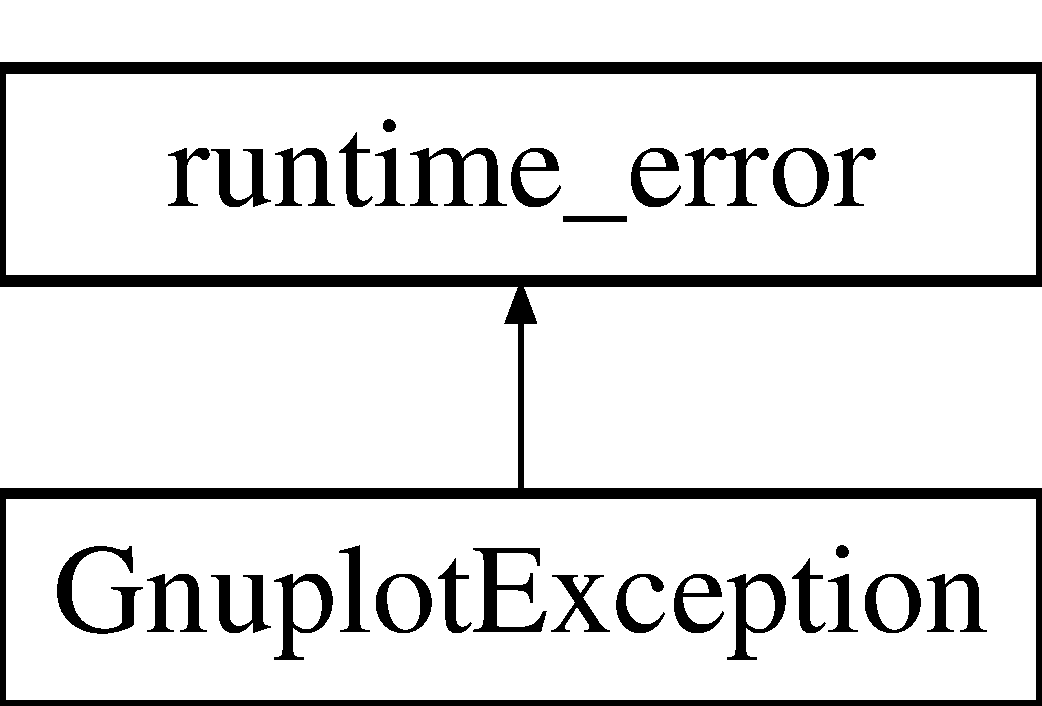
\includegraphics[height=2.000000cm]{class_gnuplot_exception}
\end{center}
\end{figure}
\subsection*{Public Member Functions}
\begin{DoxyCompactItemize}
\item 
\hyperlink{class_gnuplot_exception_a81fc74a5c019556a4d0ba2a042a63448}{Gnuplot\+Exception} (const string \&msg)
\end{DoxyCompactItemize}


\subsection{Constructor \& Destructor Documentation}
\index{Gnuplot\+Exception@{Gnuplot\+Exception}!Gnuplot\+Exception@{Gnuplot\+Exception}}
\index{Gnuplot\+Exception@{Gnuplot\+Exception}!Gnuplot\+Exception@{Gnuplot\+Exception}}
\subsubsection[{\texorpdfstring{Gnuplot\+Exception(const string \&msg)}{GnuplotException(const string &msg)}}]{\setlength{\rightskip}{0pt plus 5cm}Gnuplot\+Exception\+::\+Gnuplot\+Exception (
\begin{DoxyParamCaption}
\item[{const string \&}]{msg}
\end{DoxyParamCaption}
)\hspace{0.3cm}{\ttfamily [inline]}}\hypertarget{class_gnuplot_exception_a81fc74a5c019556a4d0ba2a042a63448}{}\label{class_gnuplot_exception_a81fc74a5c019556a4d0ba2a042a63448}


The documentation for this class was generated from the following file\+:\begin{DoxyCompactItemize}
\item 
/home/doberle/\+Advanced C\+F\+D/acfd/\+Code/\hyperlink{gnuplot__i_8h}{gnuplot\+\_\+i.\+h}\end{DoxyCompactItemize}

\hypertarget{class_grid}{}\section{Grid Class Reference}
\label{class_grid}\index{Grid@{Grid}}


Class for a 3D Cartesian grid with associated fields and coefficients.  




{\ttfamily \#include $<$grid.\+h$>$}

\subsection*{Public Member Functions}
\begin{DoxyCompactItemize}
\item 
\hyperlink{class_grid_aebc7528645c82055a45734458768be3c}{Grid} (int \hyperlink{class_grid_aee3a9d9ee92ea0ae23cb9b6e4da87e71}{nv}, int \hyperlink{class_grid_a7c02ca12ca63111a78236bf0b3ea88d8}{nc}, int nx, int ny, int nz, double lx, double ly, double lz)
\item 
\hyperlink{class_grid_a3661d0a7f998caaaf8627d7a67072116}{$\sim$\+Grid} ()
\item 
int \hyperlink{class_grid_a2fa46effcf9fbe97342b52850b72ac4c}{n} (int ind) const 
\item 
int \hyperlink{class_grid_aee3a9d9ee92ea0ae23cb9b6e4da87e71}{nv} () const 
\item 
int \hyperlink{class_grid_a7c02ca12ca63111a78236bf0b3ea88d8}{nc} () const 
\item 
double $\ast$\& \hyperlink{class_grid_a0f9d59290314e420e7adecfd6e55769c}{c} (int i, int j, int k)
\item 
double $\ast$\& \hyperlink{class_grid_ae0242e4a6d23d49e6f0382024c8f09f3}{q} (int i, int j, int k)
\item 
double $\ast$\& \hyperlink{class_grid_a68bb38f78d5f58d3dd04aa8346e8af80}{rhs} (int i, int j, int k)
\item 
double $\ast$\& \hyperlink{class_grid_af0e0caeaf47e389ea9ec154c84143ee2}{diag} (int i, int j, int k)
\item 
double $\ast$\& \hyperlink{class_grid_a8f28cebc79e45a246b2292573c988fb2}{u} (int i, int j, int k)
\item 
double $\ast$\& \hyperlink{class_grid_a91e327bd3db5b3bc85b20ad1173440d1}{f} (int dir, int i, int j, int k)
\item 
double \& \hyperlink{class_grid_ae74093daa7e9bafe77591f9336eaa409}{x} (int dir, int i, int j, int k)
\item 
double \hyperlink{class_grid_a25a0af18201fb7b20335fe745f931b1e}{dx} (int dir) const 
\item 
double \hyperlink{class_grid_ac29ca7c86c12fd0e6f1e9e5cf14c56c5}{length} (int dir) const 
\item 
int \hyperlink{class_grid_a42714a91c55d99a126b06243ecb2a673}{periodic\+\_\+index} (int i, int offset, int dir) const 
\end{DoxyCompactItemize}
\subsection*{Private Attributes}
\begin{DoxyCompactItemize}
\item 
int \hyperlink{class_grid_a41b2d78ec79a5e02aca5ae5d7211015f}{\+\_\+n} \mbox{[}3\mbox{]}
\item 
int \hyperlink{class_grid_a544a46153d54c24eb7b1a54a5e49ef04}{\+\_\+nv}
\item 
int \hyperlink{class_grid_a479b4a8777c7f8715345b1c60cf55786}{\+\_\+nc}
\item 
double $\ast$ \hyperlink{class_grid_ad1c8bee84202faab01651a41ff338368}{\+\_\+x}
\item 
double $\ast$$\ast$ \hyperlink{class_grid_a2c97df8d4d7dff67919203615bcf4cdf}{\+\_\+u}
\item 
double $\ast$$\ast$ \hyperlink{class_grid_aa4c430971c64d8181e721b9d9a495ae5}{\+\_\+c}
\item 
double $\ast$$\ast$ \hyperlink{class_grid_a5a7d695ace939b99ed0a3490ce6d80b1}{\+\_\+f}
\item 
double $\ast$$\ast$ \hyperlink{class_grid_af72acfe0e5317f83511031b9087cf2d7}{\+\_\+q}
\item 
double $\ast$$\ast$ \hyperlink{class_grid_ad94a4098427b717c50108c49d4caa048}{\+\_\+rhs}
\item 
double $\ast$$\ast$ \hyperlink{class_grid_a8476f98ceb01a28eed949abfc1123478}{\+\_\+diag}
\item 
double \hyperlink{class_grid_a34b81976f4c80eb2641224886bb6a339}{\+\_\+dx} \mbox{[}3\mbox{]}
\end{DoxyCompactItemize}


\subsection{Detailed Description}
Class for a 3D Cartesian grid with associated fields and coefficients. 


\begin{DoxyItemize}
\item dimensions nx x ny x nz
\item nv dependent variables
\item nc coefficients
\item domain size of lx x ly x lz 
\end{DoxyItemize}

\subsection{Constructor \& Destructor Documentation}
\index{Grid@{Grid}!Grid@{Grid}}
\index{Grid@{Grid}!Grid@{Grid}}
\subsubsection[{\texorpdfstring{Grid(int nv, int nc, int nx, int ny, int nz, double lx, double ly, double lz)}{Grid(int nv, int nc, int nx, int ny, int nz, double lx, double ly, double lz)}}]{\setlength{\rightskip}{0pt plus 5cm}Grid\+::\+Grid (
\begin{DoxyParamCaption}
\item[{int}]{nv, }
\item[{int}]{nc, }
\item[{int}]{nx, }
\item[{int}]{ny, }
\item[{int}]{nz, }
\item[{double}]{lx, }
\item[{double}]{ly, }
\item[{double}]{lz}
\end{DoxyParamCaption}
)}\hypertarget{class_grid_aebc7528645c82055a45734458768be3c}{}\label{class_grid_aebc7528645c82055a45734458768be3c}
\hyperlink{class_grid}{Grid} constructor 
\begin{DoxyParams}{Parameters}
{\em nv} & Number of dependent variables \\
\hline
{\em nc} & Number of coefficients \\
\hline
{\em nx,ny,nz} & Dimensions\+: nx x ny x nz \\
\hline
{\em lx,ly,lz} & Domain size\+: lx x ly x lz \\
\hline
\end{DoxyParams}
\index{Grid@{Grid}!````~Grid@{$\sim$\+Grid}}
\index{````~Grid@{$\sim$\+Grid}!Grid@{Grid}}
\subsubsection[{\texorpdfstring{$\sim$\+Grid()}{~Grid()}}]{\setlength{\rightskip}{0pt plus 5cm}Grid\+::$\sim$\+Grid (
\begin{DoxyParamCaption}
{}
\end{DoxyParamCaption}
)}\hypertarget{class_grid_a3661d0a7f998caaaf8627d7a67072116}{}\label{class_grid_a3661d0a7f998caaaf8627d7a67072116}
\hyperlink{class_grid}{Grid} destructor 

\subsection{Member Function Documentation}
\index{Grid@{Grid}!c@{c}}
\index{c@{c}!Grid@{Grid}}
\subsubsection[{\texorpdfstring{c(int i, int j, int k)}{c(int i, int j, int k)}}]{\setlength{\rightskip}{0pt plus 5cm}double$\ast$\& Grid\+::c (
\begin{DoxyParamCaption}
\item[{int}]{i, }
\item[{int}]{j, }
\item[{int}]{k}
\end{DoxyParamCaption}
)\hspace{0.3cm}{\ttfamily [inline]}}\hypertarget{class_grid_a0f9d59290314e420e7adecfd6e55769c}{}\label{class_grid_a0f9d59290314e420e7adecfd6e55769c}
Read/write access to fields using index triplets \index{Grid@{Grid}!diag@{diag}}
\index{diag@{diag}!Grid@{Grid}}
\subsubsection[{\texorpdfstring{diag(int i, int j, int k)}{diag(int i, int j, int k)}}]{\setlength{\rightskip}{0pt plus 5cm}double$\ast$\& Grid\+::diag (
\begin{DoxyParamCaption}
\item[{int}]{i, }
\item[{int}]{j, }
\item[{int}]{k}
\end{DoxyParamCaption}
)\hspace{0.3cm}{\ttfamily [inline]}}\hypertarget{class_grid_af0e0caeaf47e389ea9ec154c84143ee2}{}\label{class_grid_af0e0caeaf47e389ea9ec154c84143ee2}
\index{Grid@{Grid}!dx@{dx}}
\index{dx@{dx}!Grid@{Grid}}
\subsubsection[{\texorpdfstring{dx(int dir) const }{dx(int dir) const }}]{\setlength{\rightskip}{0pt plus 5cm}double Grid\+::dx (
\begin{DoxyParamCaption}
\item[{int}]{dir}
\end{DoxyParamCaption}
) const\hspace{0.3cm}{\ttfamily [inline]}}\hypertarget{class_grid_a25a0af18201fb7b20335fe745f931b1e}{}\label{class_grid_a25a0af18201fb7b20335fe745f931b1e}
Uniform grid spacings dx(0), dx(1) and dx(2) in x-\/, y-\/ and z-\/directions, respectively \index{Grid@{Grid}!f@{f}}
\index{f@{f}!Grid@{Grid}}
\subsubsection[{\texorpdfstring{f(int dir, int i, int j, int k)}{f(int dir, int i, int j, int k)}}]{\setlength{\rightskip}{0pt plus 5cm}double$\ast$\& Grid\+::f (
\begin{DoxyParamCaption}
\item[{int}]{dir, }
\item[{int}]{i, }
\item[{int}]{j, }
\item[{int}]{k}
\end{DoxyParamCaption}
)\hspace{0.3cm}{\ttfamily [inline]}}\hypertarget{class_grid_a91e327bd3db5b3bc85b20ad1173440d1}{}\label{class_grid_a91e327bd3db5b3bc85b20ad1173440d1}
\index{Grid@{Grid}!length@{length}}
\index{length@{length}!Grid@{Grid}}
\subsubsection[{\texorpdfstring{length(int dir) const }{length(int dir) const }}]{\setlength{\rightskip}{0pt plus 5cm}double Grid\+::length (
\begin{DoxyParamCaption}
\item[{int}]{dir}
\end{DoxyParamCaption}
) const\hspace{0.3cm}{\ttfamily [inline]}}\hypertarget{class_grid_ac29ca7c86c12fd0e6f1e9e5cf14c56c5}{}\label{class_grid_ac29ca7c86c12fd0e6f1e9e5cf14c56c5}
Domain length in x-\/, y-\/ and z-\/directions, respectively \index{Grid@{Grid}!n@{n}}
\index{n@{n}!Grid@{Grid}}
\subsubsection[{\texorpdfstring{n(int ind) const }{n(int ind) const }}]{\setlength{\rightskip}{0pt plus 5cm}int Grid\+::n (
\begin{DoxyParamCaption}
\item[{int}]{ind}
\end{DoxyParamCaption}
) const\hspace{0.3cm}{\ttfamily [inline]}}\hypertarget{class_grid_a2fa46effcf9fbe97342b52850b72ac4c}{}\label{class_grid_a2fa46effcf9fbe97342b52850b72ac4c}
Dimensions\+: n(0) x n(1) x n(2) \index{Grid@{Grid}!nc@{nc}}
\index{nc@{nc}!Grid@{Grid}}
\subsubsection[{\texorpdfstring{nc() const }{nc() const }}]{\setlength{\rightskip}{0pt plus 5cm}int Grid\+::nc (
\begin{DoxyParamCaption}
{}
\end{DoxyParamCaption}
) const\hspace{0.3cm}{\ttfamily [inline]}}\hypertarget{class_grid_a7c02ca12ca63111a78236bf0b3ea88d8}{}\label{class_grid_a7c02ca12ca63111a78236bf0b3ea88d8}
Number of coefficients \index{Grid@{Grid}!nv@{nv}}
\index{nv@{nv}!Grid@{Grid}}
\subsubsection[{\texorpdfstring{nv() const }{nv() const }}]{\setlength{\rightskip}{0pt plus 5cm}int Grid\+::nv (
\begin{DoxyParamCaption}
{}
\end{DoxyParamCaption}
) const\hspace{0.3cm}{\ttfamily [inline]}}\hypertarget{class_grid_aee3a9d9ee92ea0ae23cb9b6e4da87e71}{}\label{class_grid_aee3a9d9ee92ea0ae23cb9b6e4da87e71}
Number of dependent variable \index{Grid@{Grid}!periodic\+\_\+index@{periodic\+\_\+index}}
\index{periodic\+\_\+index@{periodic\+\_\+index}!Grid@{Grid}}
\subsubsection[{\texorpdfstring{periodic\+\_\+index(int i, int offset, int dir) const }{periodic_index(int i, int offset, int dir) const }}]{\setlength{\rightskip}{0pt plus 5cm}int Grid\+::periodic\+\_\+index (
\begin{DoxyParamCaption}
\item[{int}]{i, }
\item[{int}]{offset, }
\item[{int}]{dir}
\end{DoxyParamCaption}
) const\hspace{0.3cm}{\ttfamily [inline]}}\hypertarget{class_grid_a42714a91c55d99a126b06243ecb2a673}{}\label{class_grid_a42714a91c55d99a126b06243ecb2a673}
Computation of index with an offset, using domain periodicity if (i + offset) is smaller than 0 or great than n(dir)-\/1. 
\begin{DoxyParams}{Parameters}
{\em i} & Index \\
\hline
{\em offset} & Offset with respect to i \\
\hline
{\em dir} & Coordinate axis \\
\hline
\end{DoxyParams}
\index{Grid@{Grid}!q@{q}}
\index{q@{q}!Grid@{Grid}}
\subsubsection[{\texorpdfstring{q(int i, int j, int k)}{q(int i, int j, int k)}}]{\setlength{\rightskip}{0pt plus 5cm}double$\ast$\& Grid\+::q (
\begin{DoxyParamCaption}
\item[{int}]{i, }
\item[{int}]{j, }
\item[{int}]{k}
\end{DoxyParamCaption}
)\hspace{0.3cm}{\ttfamily [inline]}}\hypertarget{class_grid_ae0242e4a6d23d49e6f0382024c8f09f3}{}\label{class_grid_ae0242e4a6d23d49e6f0382024c8f09f3}
\index{Grid@{Grid}!rhs@{rhs}}
\index{rhs@{rhs}!Grid@{Grid}}
\subsubsection[{\texorpdfstring{rhs(int i, int j, int k)}{rhs(int i, int j, int k)}}]{\setlength{\rightskip}{0pt plus 5cm}double$\ast$\& Grid\+::rhs (
\begin{DoxyParamCaption}
\item[{int}]{i, }
\item[{int}]{j, }
\item[{int}]{k}
\end{DoxyParamCaption}
)\hspace{0.3cm}{\ttfamily [inline]}}\hypertarget{class_grid_a68bb38f78d5f58d3dd04aa8346e8af80}{}\label{class_grid_a68bb38f78d5f58d3dd04aa8346e8af80}
\index{Grid@{Grid}!u@{u}}
\index{u@{u}!Grid@{Grid}}
\subsubsection[{\texorpdfstring{u(int i, int j, int k)}{u(int i, int j, int k)}}]{\setlength{\rightskip}{0pt plus 5cm}double$\ast$\& Grid\+::u (
\begin{DoxyParamCaption}
\item[{int}]{i, }
\item[{int}]{j, }
\item[{int}]{k}
\end{DoxyParamCaption}
)\hspace{0.3cm}{\ttfamily [inline]}}\hypertarget{class_grid_a8f28cebc79e45a246b2292573c988fb2}{}\label{class_grid_a8f28cebc79e45a246b2292573c988fb2}
\index{Grid@{Grid}!x@{x}}
\index{x@{x}!Grid@{Grid}}
\subsubsection[{\texorpdfstring{x(int dir, int i, int j, int k)}{x(int dir, int i, int j, int k)}}]{\setlength{\rightskip}{0pt plus 5cm}double\& Grid\+::x (
\begin{DoxyParamCaption}
\item[{int}]{dir, }
\item[{int}]{i, }
\item[{int}]{j, }
\item[{int}]{k}
\end{DoxyParamCaption}
)\hspace{0.3cm}{\ttfamily [inline]}}\hypertarget{class_grid_ae74093daa7e9bafe77591f9336eaa409}{}\label{class_grid_ae74093daa7e9bafe77591f9336eaa409}
Coordinates (x,y,z) = (x(0,i,j,k),x(1,i,j,k),x(2,i,j,k) for each grid node (i,j,k) 

\subsection{Member Data Documentation}
\index{Grid@{Grid}!\+\_\+c@{\+\_\+c}}
\index{\+\_\+c@{\+\_\+c}!Grid@{Grid}}
\subsubsection[{\texorpdfstring{\+\_\+c}{_c}}]{\setlength{\rightskip}{0pt plus 5cm}double$\ast$$\ast$ Grid\+::\+\_\+c\hspace{0.3cm}{\ttfamily [private]}}\hypertarget{class_grid_aa4c430971c64d8181e721b9d9a495ae5}{}\label{class_grid_aa4c430971c64d8181e721b9d9a495ae5}
\index{Grid@{Grid}!\+\_\+diag@{\+\_\+diag}}
\index{\+\_\+diag@{\+\_\+diag}!Grid@{Grid}}
\subsubsection[{\texorpdfstring{\+\_\+diag}{_diag}}]{\setlength{\rightskip}{0pt plus 5cm}double$\ast$$\ast$ Grid\+::\+\_\+diag\hspace{0.3cm}{\ttfamily [private]}}\hypertarget{class_grid_a8476f98ceb01a28eed949abfc1123478}{}\label{class_grid_a8476f98ceb01a28eed949abfc1123478}
\index{Grid@{Grid}!\+\_\+dx@{\+\_\+dx}}
\index{\+\_\+dx@{\+\_\+dx}!Grid@{Grid}}
\subsubsection[{\texorpdfstring{\+\_\+dx}{_dx}}]{\setlength{\rightskip}{0pt plus 5cm}double Grid\+::\+\_\+dx\mbox{[}3\mbox{]}\hspace{0.3cm}{\ttfamily [private]}}\hypertarget{class_grid_a34b81976f4c80eb2641224886bb6a339}{}\label{class_grid_a34b81976f4c80eb2641224886bb6a339}
\index{Grid@{Grid}!\+\_\+f@{\+\_\+f}}
\index{\+\_\+f@{\+\_\+f}!Grid@{Grid}}
\subsubsection[{\texorpdfstring{\+\_\+f}{_f}}]{\setlength{\rightskip}{0pt plus 5cm}double$\ast$$\ast$ Grid\+::\+\_\+f\hspace{0.3cm}{\ttfamily [private]}}\hypertarget{class_grid_a5a7d695ace939b99ed0a3490ce6d80b1}{}\label{class_grid_a5a7d695ace939b99ed0a3490ce6d80b1}
\index{Grid@{Grid}!\+\_\+n@{\+\_\+n}}
\index{\+\_\+n@{\+\_\+n}!Grid@{Grid}}
\subsubsection[{\texorpdfstring{\+\_\+n}{_n}}]{\setlength{\rightskip}{0pt plus 5cm}int Grid\+::\+\_\+n\mbox{[}3\mbox{]}\hspace{0.3cm}{\ttfamily [private]}}\hypertarget{class_grid_a41b2d78ec79a5e02aca5ae5d7211015f}{}\label{class_grid_a41b2d78ec79a5e02aca5ae5d7211015f}
\index{Grid@{Grid}!\+\_\+nc@{\+\_\+nc}}
\index{\+\_\+nc@{\+\_\+nc}!Grid@{Grid}}
\subsubsection[{\texorpdfstring{\+\_\+nc}{_nc}}]{\setlength{\rightskip}{0pt plus 5cm}int Grid\+::\+\_\+nc\hspace{0.3cm}{\ttfamily [private]}}\hypertarget{class_grid_a479b4a8777c7f8715345b1c60cf55786}{}\label{class_grid_a479b4a8777c7f8715345b1c60cf55786}
\index{Grid@{Grid}!\+\_\+nv@{\+\_\+nv}}
\index{\+\_\+nv@{\+\_\+nv}!Grid@{Grid}}
\subsubsection[{\texorpdfstring{\+\_\+nv}{_nv}}]{\setlength{\rightskip}{0pt plus 5cm}int Grid\+::\+\_\+nv\hspace{0.3cm}{\ttfamily [private]}}\hypertarget{class_grid_a544a46153d54c24eb7b1a54a5e49ef04}{}\label{class_grid_a544a46153d54c24eb7b1a54a5e49ef04}
\index{Grid@{Grid}!\+\_\+q@{\+\_\+q}}
\index{\+\_\+q@{\+\_\+q}!Grid@{Grid}}
\subsubsection[{\texorpdfstring{\+\_\+q}{_q}}]{\setlength{\rightskip}{0pt plus 5cm}double$\ast$$\ast$ Grid\+::\+\_\+q\hspace{0.3cm}{\ttfamily [private]}}\hypertarget{class_grid_af72acfe0e5317f83511031b9087cf2d7}{}\label{class_grid_af72acfe0e5317f83511031b9087cf2d7}
\index{Grid@{Grid}!\+\_\+rhs@{\+\_\+rhs}}
\index{\+\_\+rhs@{\+\_\+rhs}!Grid@{Grid}}
\subsubsection[{\texorpdfstring{\+\_\+rhs}{_rhs}}]{\setlength{\rightskip}{0pt plus 5cm}double$\ast$$\ast$ Grid\+::\+\_\+rhs\hspace{0.3cm}{\ttfamily [private]}}\hypertarget{class_grid_ad94a4098427b717c50108c49d4caa048}{}\label{class_grid_ad94a4098427b717c50108c49d4caa048}
\index{Grid@{Grid}!\+\_\+u@{\+\_\+u}}
\index{\+\_\+u@{\+\_\+u}!Grid@{Grid}}
\subsubsection[{\texorpdfstring{\+\_\+u}{_u}}]{\setlength{\rightskip}{0pt plus 5cm}double$\ast$$\ast$ Grid\+::\+\_\+u\hspace{0.3cm}{\ttfamily [private]}}\hypertarget{class_grid_a2c97df8d4d7dff67919203615bcf4cdf}{}\label{class_grid_a2c97df8d4d7dff67919203615bcf4cdf}
\index{Grid@{Grid}!\+\_\+x@{\+\_\+x}}
\index{\+\_\+x@{\+\_\+x}!Grid@{Grid}}
\subsubsection[{\texorpdfstring{\+\_\+x}{_x}}]{\setlength{\rightskip}{0pt plus 5cm}double$\ast$ Grid\+::\+\_\+x\hspace{0.3cm}{\ttfamily [private]}}\hypertarget{class_grid_ad1c8bee84202faab01651a41ff338368}{}\label{class_grid_ad1c8bee84202faab01651a41ff338368}


The documentation for this class was generated from the following files\+:\begin{DoxyCompactItemize}
\item 
/home/doberle/\+Advanced C\+F\+D/acfd/\+Code/\hyperlink{grid_8h}{grid.\+h}\item 
/home/doberle/\+Advanced C\+F\+D/acfd/\+Code/\hyperlink{grid_8cpp}{grid.\+cpp}\end{DoxyCompactItemize}

\hypertarget{class_init}{}\section{Init Class Reference}
\label{class_init}\index{Init@{Init}}


Abstract class for the definition of initial conditions for fields defined on a \hyperlink{class_grid}{Grid} object.  




{\ttfamily \#include $<$init.\+h$>$}

Inheritance diagram for Init\+:\begin{figure}[H]
\begin{center}
\leavevmode
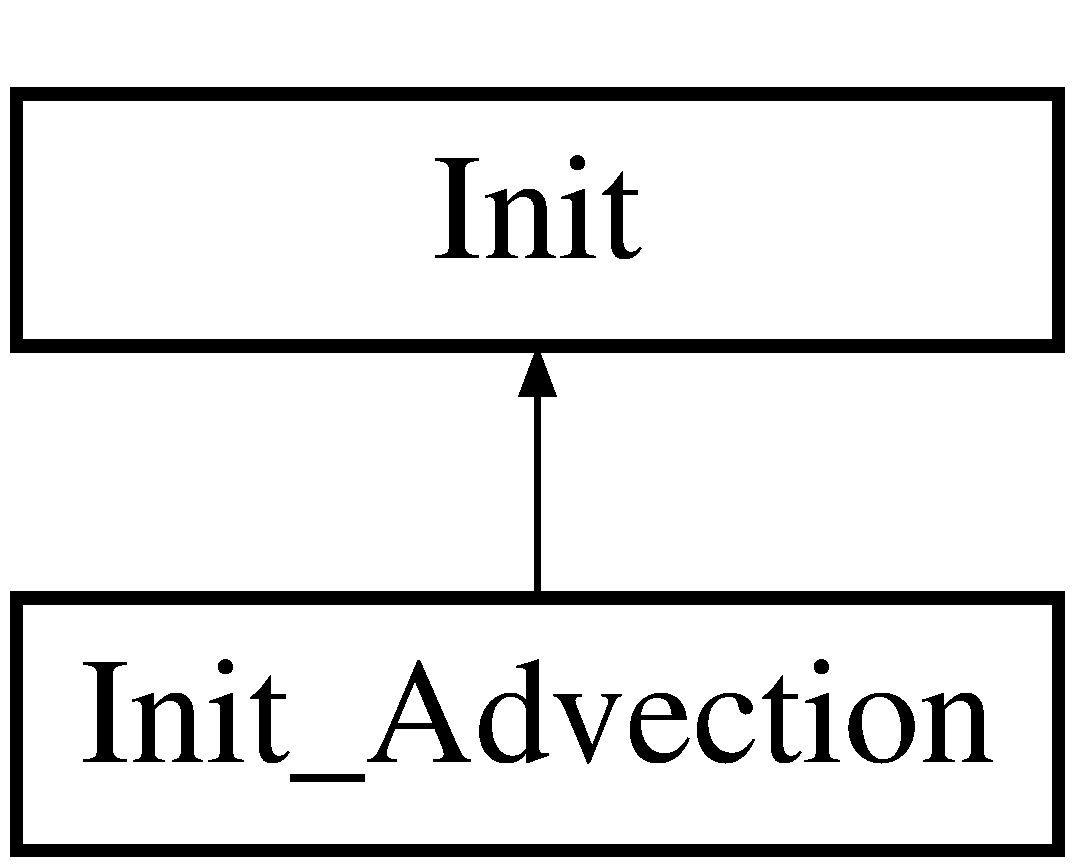
\includegraphics[height=2.000000cm]{class_init}
\end{center}
\end{figure}
\subsection*{Public Member Functions}
\begin{DoxyCompactItemize}
\item 
\hyperlink{class_init_aaf14d36f1120460e411f35b54a3bd385}{Init} (\hyperlink{class_control}{Control} $\ast$c)
\item 
virtual \hyperlink{class_init_adf301c6b7bfd8c50032fe2cfef0b102e}{$\sim$\+Init} ()
\item 
virtual void \hyperlink{class_init_a1deef07e59de84489cbf7a10d2e737d2}{operator()} (\hyperlink{class_grid}{Grid} $\ast$g) const =0
\end{DoxyCompactItemize}
\subsection*{Protected Attributes}
\begin{DoxyCompactItemize}
\item 
\hyperlink{class_control}{Control} $\ast$ \hyperlink{class_init_a0e16042aa3fadf50ccf598d0d255cd36}{\+\_\+c}
\end{DoxyCompactItemize}


\subsection{Detailed Description}
Abstract class for the definition of initial conditions for fields defined on a \hyperlink{class_grid}{Grid} object. 

\subsection{Constructor \& Destructor Documentation}
\index{Init@{Init}!Init@{Init}}
\index{Init@{Init}!Init@{Init}}
\subsubsection[{\texorpdfstring{Init(\+Control $\ast$c)}{Init(Control *c)}}]{\setlength{\rightskip}{0pt plus 5cm}Init\+::\+Init (
\begin{DoxyParamCaption}
\item[{{\bf Control} $\ast$}]{c}
\end{DoxyParamCaption}
)\hspace{0.3cm}{\ttfamily [inline]}}\hypertarget{class_init_aaf14d36f1120460e411f35b54a3bd385}{}\label{class_init_aaf14d36f1120460e411f35b54a3bd385}
\index{Init@{Init}!````~Init@{$\sim$\+Init}}
\index{````~Init@{$\sim$\+Init}!Init@{Init}}
\subsubsection[{\texorpdfstring{$\sim$\+Init()}{~Init()}}]{\setlength{\rightskip}{0pt plus 5cm}virtual Init\+::$\sim$\+Init (
\begin{DoxyParamCaption}
{}
\end{DoxyParamCaption}
)\hspace{0.3cm}{\ttfamily [inline]}, {\ttfamily [virtual]}}\hypertarget{class_init_adf301c6b7bfd8c50032fe2cfef0b102e}{}\label{class_init_adf301c6b7bfd8c50032fe2cfef0b102e}


\subsection{Member Function Documentation}
\index{Init@{Init}!operator()@{operator()}}
\index{operator()@{operator()}!Init@{Init}}
\subsubsection[{\texorpdfstring{operator()(\+Grid $\ast$g) const =0}{operator()(Grid *g) const =0}}]{\setlength{\rightskip}{0pt plus 5cm}virtual void Init\+::operator() (
\begin{DoxyParamCaption}
\item[{{\bf Grid} $\ast$}]{g}
\end{DoxyParamCaption}
) const\hspace{0.3cm}{\ttfamily [pure virtual]}}\hypertarget{class_init_a1deef07e59de84489cbf7a10d2e737d2}{}\label{class_init_a1deef07e59de84489cbf7a10d2e737d2}
Defines the initial condition given an entry in the control file 

Implemented in \hyperlink{class_init___advection_a336eaeee433ab0ec8a17eb61b9a17c41}{Init\+\_\+\+Advection}.



\subsection{Member Data Documentation}
\index{Init@{Init}!\+\_\+c@{\+\_\+c}}
\index{\+\_\+c@{\+\_\+c}!Init@{Init}}
\subsubsection[{\texorpdfstring{\+\_\+c}{_c}}]{\setlength{\rightskip}{0pt plus 5cm}{\bf Control}$\ast$ Init\+::\+\_\+c\hspace{0.3cm}{\ttfamily [protected]}}\hypertarget{class_init_a0e16042aa3fadf50ccf598d0d255cd36}{}\label{class_init_a0e16042aa3fadf50ccf598d0d255cd36}


The documentation for this class was generated from the following file\+:\begin{DoxyCompactItemize}
\item 
/home/doberle/\+Advanced C\+F\+D/acfd/\+Code/\hyperlink{init_8h}{init.\+h}\end{DoxyCompactItemize}

\hypertarget{class_init___advection}{}\section{Init\+\_\+\+Advection Class Reference}
\label{class_init___advection}\index{Init\+\_\+\+Advection@{Init\+\_\+\+Advection}}


Initial condition for the linear advection-\/diffusion equation.  




{\ttfamily \#include $<$init\+\_\+advection.\+h$>$}

Inheritance diagram for Init\+\_\+\+Advection\+:\begin{figure}[H]
\begin{center}
\leavevmode
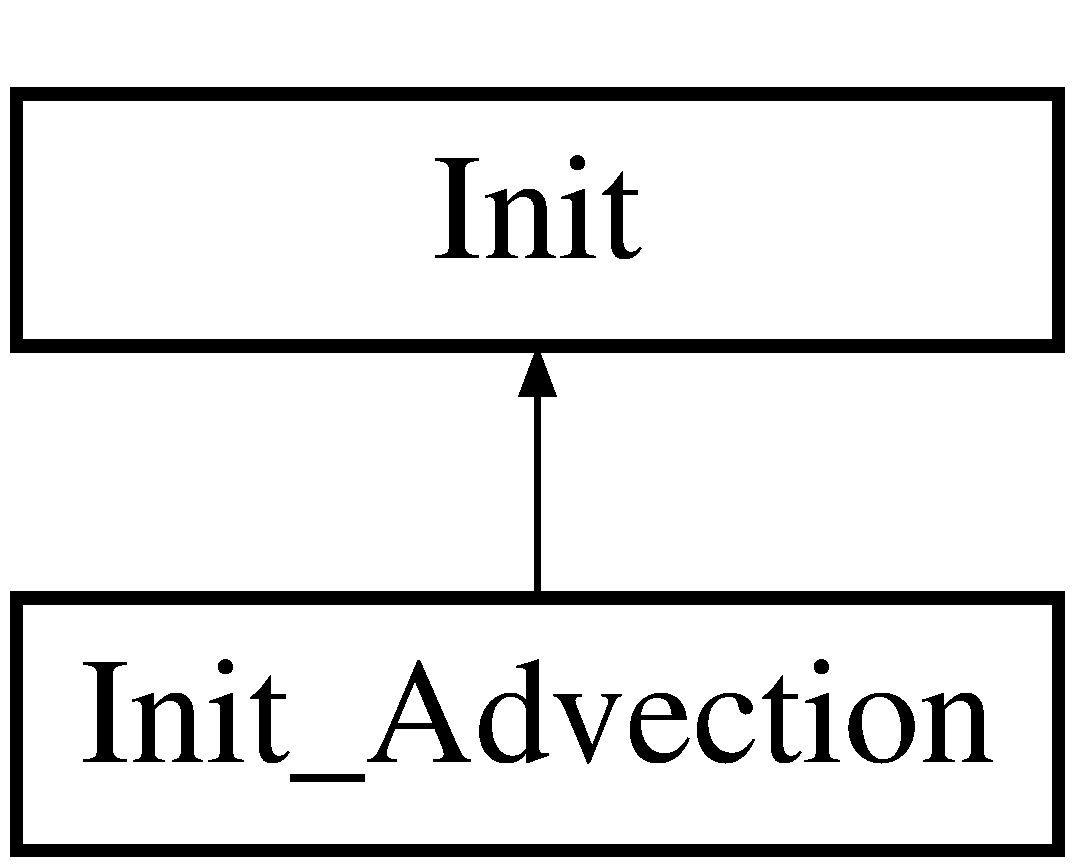
\includegraphics[height=2.000000cm]{class_init___advection}
\end{center}
\end{figure}
\subsection*{Public Member Functions}
\begin{DoxyCompactItemize}
\item 
\hyperlink{class_init___advection_a7d15ce87d291abaddcd0dad556cb9469}{Init\+\_\+\+Advection} (\hyperlink{class_control}{Control} $\ast$c)
\item 
\hyperlink{class_init___advection_a4defc25e1485a0f8f8172ba2c45e8950}{$\sim$\+Init\+\_\+\+Advection} ()
\item 
void \hyperlink{class_init___advection_a336eaeee433ab0ec8a17eb61b9a17c41}{operator()} (\hyperlink{class_grid}{Grid} $\ast$g) const 
\end{DoxyCompactItemize}
\subsection*{Private Member Functions}
\begin{DoxyCompactItemize}
\item 
void \hyperlink{class_init___advection_a713f4d7ad7652070e41d995521d1b5ff}{init\+\_\+1d\+\_\+tophat} (\hyperlink{class_grid}{Grid} $\ast$g) const 
\item 
void \hyperlink{class_init___advection_a40cb7002a9a849adb5d9d7c9bca3e07e}{init\+\_\+1d\+\_\+sin} (\hyperlink{class_grid}{Grid} $\ast$g) const 
\item 
void \hyperlink{class_init___advection_a8100aa1f38bb3a9684e410b2ea167b8e}{init\+\_\+2d\+\_\+tophat} (\hyperlink{class_grid}{Grid} $\ast$g) const 
\item 
void \hyperlink{class_init___advection_a9dbd1a325e26cf02eac47fb45b980dbb}{init\+\_\+2d\+\_\+sin} (\hyperlink{class_grid}{Grid} $\ast$g) const 
\end{DoxyCompactItemize}
\subsection*{Additional Inherited Members}


\subsection{Detailed Description}
Initial condition for the linear advection-\/diffusion equation. 

\subsection{Constructor \& Destructor Documentation}
\index{Init\+\_\+\+Advection@{Init\+\_\+\+Advection}!Init\+\_\+\+Advection@{Init\+\_\+\+Advection}}
\index{Init\+\_\+\+Advection@{Init\+\_\+\+Advection}!Init\+\_\+\+Advection@{Init\+\_\+\+Advection}}
\subsubsection[{\texorpdfstring{Init\+\_\+\+Advection(\+Control $\ast$c)}{Init_Advection(Control *c)}}]{\setlength{\rightskip}{0pt plus 5cm}Init\+\_\+\+Advection\+::\+Init\+\_\+\+Advection (
\begin{DoxyParamCaption}
\item[{{\bf Control} $\ast$}]{c}
\end{DoxyParamCaption}
)\hspace{0.3cm}{\ttfamily [inline]}}\hypertarget{class_init___advection_a7d15ce87d291abaddcd0dad556cb9469}{}\label{class_init___advection_a7d15ce87d291abaddcd0dad556cb9469}
\index{Init\+\_\+\+Advection@{Init\+\_\+\+Advection}!````~Init\+\_\+\+Advection@{$\sim$\+Init\+\_\+\+Advection}}
\index{````~Init\+\_\+\+Advection@{$\sim$\+Init\+\_\+\+Advection}!Init\+\_\+\+Advection@{Init\+\_\+\+Advection}}
\subsubsection[{\texorpdfstring{$\sim$\+Init\+\_\+\+Advection()}{~Init_Advection()}}]{\setlength{\rightskip}{0pt plus 5cm}Init\+\_\+\+Advection\+::$\sim$\+Init\+\_\+\+Advection (
\begin{DoxyParamCaption}
{}
\end{DoxyParamCaption}
)\hspace{0.3cm}{\ttfamily [inline]}}\hypertarget{class_init___advection_a4defc25e1485a0f8f8172ba2c45e8950}{}\label{class_init___advection_a4defc25e1485a0f8f8172ba2c45e8950}


\subsection{Member Function Documentation}
\index{Init\+\_\+\+Advection@{Init\+\_\+\+Advection}!init\+\_\+1d\+\_\+sin@{init\+\_\+1d\+\_\+sin}}
\index{init\+\_\+1d\+\_\+sin@{init\+\_\+1d\+\_\+sin}!Init\+\_\+\+Advection@{Init\+\_\+\+Advection}}
\subsubsection[{\texorpdfstring{init\+\_\+1d\+\_\+sin(\+Grid $\ast$g) const }{init_1d_sin(Grid *g) const }}]{\setlength{\rightskip}{0pt plus 5cm}void Init\+\_\+\+Advection\+::init\+\_\+1d\+\_\+sin (
\begin{DoxyParamCaption}
\item[{{\bf Grid} $\ast$}]{g}
\end{DoxyParamCaption}
) const\hspace{0.3cm}{\ttfamily [private]}}\hypertarget{class_init___advection_a40cb7002a9a849adb5d9d7c9bca3e07e}{}\label{class_init___advection_a40cb7002a9a849adb5d9d7c9bca3e07e}
\index{Init\+\_\+\+Advection@{Init\+\_\+\+Advection}!init\+\_\+1d\+\_\+tophat@{init\+\_\+1d\+\_\+tophat}}
\index{init\+\_\+1d\+\_\+tophat@{init\+\_\+1d\+\_\+tophat}!Init\+\_\+\+Advection@{Init\+\_\+\+Advection}}
\subsubsection[{\texorpdfstring{init\+\_\+1d\+\_\+tophat(\+Grid $\ast$g) const }{init_1d_tophat(Grid *g) const }}]{\setlength{\rightskip}{0pt plus 5cm}void Init\+\_\+\+Advection\+::init\+\_\+1d\+\_\+tophat (
\begin{DoxyParamCaption}
\item[{{\bf Grid} $\ast$}]{g}
\end{DoxyParamCaption}
) const\hspace{0.3cm}{\ttfamily [private]}}\hypertarget{class_init___advection_a713f4d7ad7652070e41d995521d1b5ff}{}\label{class_init___advection_a713f4d7ad7652070e41d995521d1b5ff}
\index{Init\+\_\+\+Advection@{Init\+\_\+\+Advection}!init\+\_\+2d\+\_\+sin@{init\+\_\+2d\+\_\+sin}}
\index{init\+\_\+2d\+\_\+sin@{init\+\_\+2d\+\_\+sin}!Init\+\_\+\+Advection@{Init\+\_\+\+Advection}}
\subsubsection[{\texorpdfstring{init\+\_\+2d\+\_\+sin(\+Grid $\ast$g) const }{init_2d_sin(Grid *g) const }}]{\setlength{\rightskip}{0pt plus 5cm}void Init\+\_\+\+Advection\+::init\+\_\+2d\+\_\+sin (
\begin{DoxyParamCaption}
\item[{{\bf Grid} $\ast$}]{g}
\end{DoxyParamCaption}
) const\hspace{0.3cm}{\ttfamily [private]}}\hypertarget{class_init___advection_a9dbd1a325e26cf02eac47fb45b980dbb}{}\label{class_init___advection_a9dbd1a325e26cf02eac47fb45b980dbb}
\index{Init\+\_\+\+Advection@{Init\+\_\+\+Advection}!init\+\_\+2d\+\_\+tophat@{init\+\_\+2d\+\_\+tophat}}
\index{init\+\_\+2d\+\_\+tophat@{init\+\_\+2d\+\_\+tophat}!Init\+\_\+\+Advection@{Init\+\_\+\+Advection}}
\subsubsection[{\texorpdfstring{init\+\_\+2d\+\_\+tophat(\+Grid $\ast$g) const }{init_2d_tophat(Grid *g) const }}]{\setlength{\rightskip}{0pt plus 5cm}void Init\+\_\+\+Advection\+::init\+\_\+2d\+\_\+tophat (
\begin{DoxyParamCaption}
\item[{{\bf Grid} $\ast$}]{g}
\end{DoxyParamCaption}
) const\hspace{0.3cm}{\ttfamily [private]}}\hypertarget{class_init___advection_a8100aa1f38bb3a9684e410b2ea167b8e}{}\label{class_init___advection_a8100aa1f38bb3a9684e410b2ea167b8e}
\index{Init\+\_\+\+Advection@{Init\+\_\+\+Advection}!operator()@{operator()}}
\index{operator()@{operator()}!Init\+\_\+\+Advection@{Init\+\_\+\+Advection}}
\subsubsection[{\texorpdfstring{operator()(\+Grid $\ast$g) const }{operator()(Grid *g) const }}]{\setlength{\rightskip}{0pt plus 5cm}void Init\+\_\+\+Advection\+::operator() (
\begin{DoxyParamCaption}
\item[{{\bf Grid} $\ast$}]{g}
\end{DoxyParamCaption}
) const\hspace{0.3cm}{\ttfamily [inline]}, {\ttfamily [virtual]}}\hypertarget{class_init___advection_a336eaeee433ab0ec8a17eb61b9a17c41}{}\label{class_init___advection_a336eaeee433ab0ec8a17eb61b9a17c41}
Defines the initial condition given an entry in the control file.
\begin{DoxyItemize}
\item 1\+: 1D top hat
\item 2\+: 1D sine wave
\item 3\+: 2D top hat
\item 4\+: 2D sine wave 
\end{DoxyItemize}

Implements \hyperlink{class_init_a1deef07e59de84489cbf7a10d2e737d2}{Init}.



The documentation for this class was generated from the following files\+:\begin{DoxyCompactItemize}
\item 
/home/doberle/\+Advanced C\+F\+D/acfd/\+Code/\hyperlink{init__advection_8h}{init\+\_\+advection.\+h}\item 
/home/doberle/\+Advanced C\+F\+D/acfd/\+Code/\hyperlink{init__advection_8cpp}{init\+\_\+advection.\+cpp}\end{DoxyCompactItemize}

\hypertarget{class_plot}{}\section{Plot Class Reference}
\label{class_plot}\index{Plot@{Plot}}


Abstract class for plotting simulation results.  




{\ttfamily \#include $<$plot.\+h$>$}

Inheritance diagram for Plot\+:\begin{figure}[H]
\begin{center}
\leavevmode
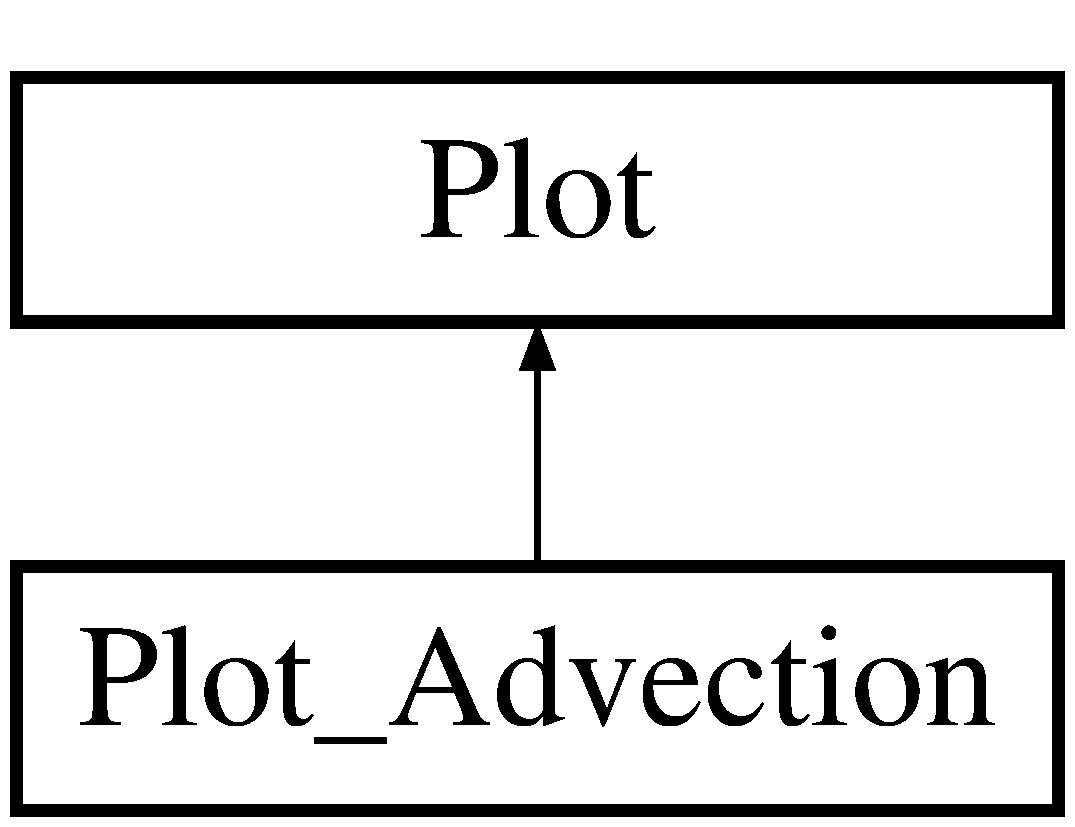
\includegraphics[height=2.000000cm]{class_plot}
\end{center}
\end{figure}
\subsection*{Public Member Functions}
\begin{DoxyCompactItemize}
\item 
\hyperlink{class_plot_a6bb02285cc339b4fd9796a0331818463}{Plot} (\hyperlink{class_control}{Control} $\ast$c)
\item 
virtual \hyperlink{class_plot_ac71811ea4362a4c03e017a7a72125e1f}{$\sim$\+Plot} ()
\item 
virtual void \hyperlink{class_plot_a0c81ddc39ad4695024eb5ed493cba26e}{operator()} (\hyperlink{class_grid}{Grid} $\ast$g)=0
\end{DoxyCompactItemize}
\subsection*{Protected Attributes}
\begin{DoxyCompactItemize}
\item 
\hyperlink{class_control}{Control} $\ast$ \hyperlink{class_plot_afde6de3bfd787193d73fe24f6a44a479}{\+\_\+c}
\end{DoxyCompactItemize}


\subsection{Detailed Description}
Abstract class for plotting simulation results. 

\subsection{Constructor \& Destructor Documentation}
\index{Plot@{Plot}!Plot@{Plot}}
\index{Plot@{Plot}!Plot@{Plot}}
\subsubsection[{\texorpdfstring{Plot(\+Control $\ast$c)}{Plot(Control *c)}}]{\setlength{\rightskip}{0pt plus 5cm}Plot\+::\+Plot (
\begin{DoxyParamCaption}
\item[{{\bf Control} $\ast$}]{c}
\end{DoxyParamCaption}
)\hspace{0.3cm}{\ttfamily [inline]}}\hypertarget{class_plot_a6bb02285cc339b4fd9796a0331818463}{}\label{class_plot_a6bb02285cc339b4fd9796a0331818463}
\index{Plot@{Plot}!````~Plot@{$\sim$\+Plot}}
\index{````~Plot@{$\sim$\+Plot}!Plot@{Plot}}
\subsubsection[{\texorpdfstring{$\sim$\+Plot()}{~Plot()}}]{\setlength{\rightskip}{0pt plus 5cm}virtual Plot\+::$\sim$\+Plot (
\begin{DoxyParamCaption}
{}
\end{DoxyParamCaption}
)\hspace{0.3cm}{\ttfamily [inline]}, {\ttfamily [virtual]}}\hypertarget{class_plot_ac71811ea4362a4c03e017a7a72125e1f}{}\label{class_plot_ac71811ea4362a4c03e017a7a72125e1f}


\subsection{Member Function Documentation}
\index{Plot@{Plot}!operator()@{operator()}}
\index{operator()@{operator()}!Plot@{Plot}}
\subsubsection[{\texorpdfstring{operator()(\+Grid $\ast$g)=0}{operator()(Grid *g)=0}}]{\setlength{\rightskip}{0pt plus 5cm}virtual void Plot\+::operator() (
\begin{DoxyParamCaption}
\item[{{\bf Grid} $\ast$}]{g}
\end{DoxyParamCaption}
)\hspace{0.3cm}{\ttfamily [pure virtual]}}\hypertarget{class_plot_a0c81ddc39ad4695024eb5ed493cba26e}{}\label{class_plot_a0c81ddc39ad4695024eb5ed493cba26e}
\hyperlink{class_plot}{Plot} simulation results given an entry in the control file. 

Implemented in \hyperlink{class_plot___advection_aa8f4020a38efe82391d6ec2c30cb2846}{Plot\+\_\+\+Advection}.



\subsection{Member Data Documentation}
\index{Plot@{Plot}!\+\_\+c@{\+\_\+c}}
\index{\+\_\+c@{\+\_\+c}!Plot@{Plot}}
\subsubsection[{\texorpdfstring{\+\_\+c}{_c}}]{\setlength{\rightskip}{0pt plus 5cm}{\bf Control}$\ast$ Plot\+::\+\_\+c\hspace{0.3cm}{\ttfamily [protected]}}\hypertarget{class_plot_afde6de3bfd787193d73fe24f6a44a479}{}\label{class_plot_afde6de3bfd787193d73fe24f6a44a479}


The documentation for this class was generated from the following file\+:\begin{DoxyCompactItemize}
\item 
/home/doberle/\+Advanced C\+F\+D/acfd/\+Code/\hyperlink{plot_8h}{plot.\+h}\end{DoxyCompactItemize}

\hypertarget{class_plot___advection}{}\section{Plot\+\_\+\+Advection Class Reference}
\label{class_plot___advection}\index{Plot\+\_\+\+Advection@{Plot\+\_\+\+Advection}}


Plotting class for the linear advection-\/diffusion equation.  




{\ttfamily \#include $<$plot\+\_\+advection.\+h$>$}

Inheritance diagram for Plot\+\_\+\+Advection\+:\begin{figure}[H]
\begin{center}
\leavevmode
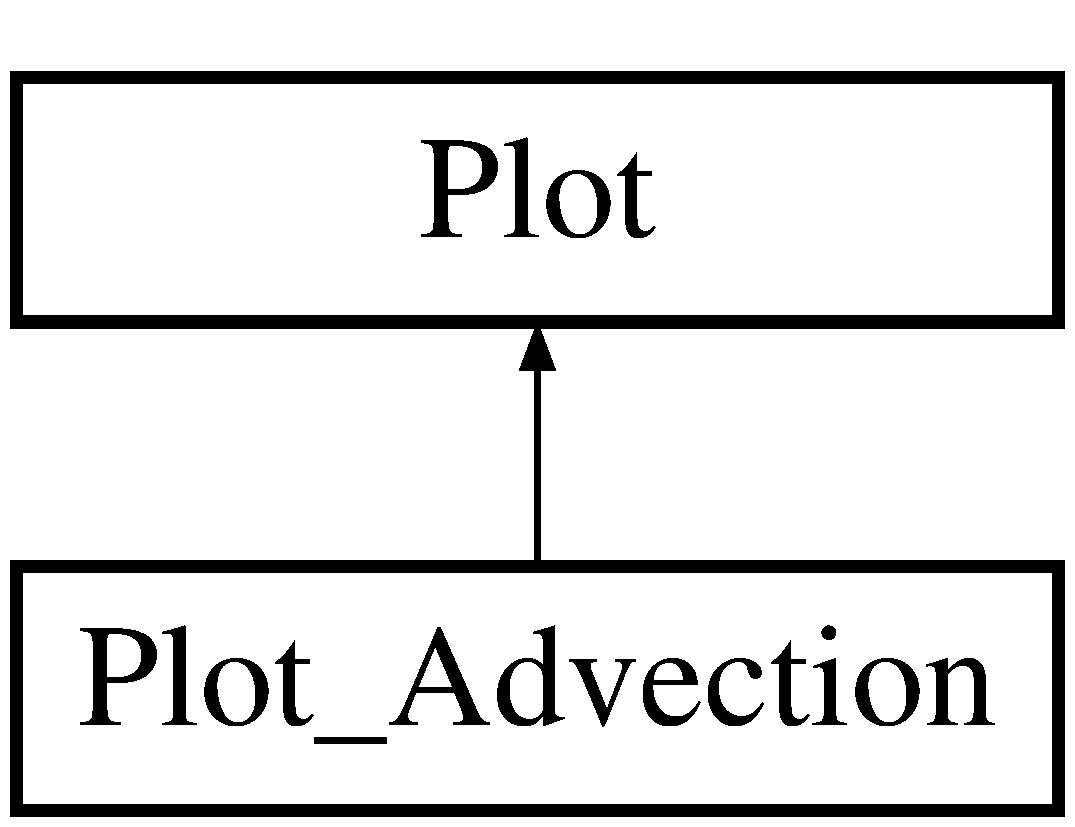
\includegraphics[height=2.000000cm]{class_plot___advection}
\end{center}
\end{figure}
\subsection*{Public Member Functions}
\begin{DoxyCompactItemize}
\item 
\hyperlink{class_plot___advection_a5d506920ee2b9b7f54382208ca31db28}{Plot\+\_\+\+Advection} (\hyperlink{class_control}{Control} $\ast$c)
\item 
\hyperlink{class_plot___advection_aa4836efc4922b4ba4f7788315d4e4994}{$\sim$\+Plot\+\_\+\+Advection} ()
\item 
void \hyperlink{class_plot___advection_aa8f4020a38efe82391d6ec2c30cb2846}{operator()} (\hyperlink{class_grid}{Grid} $\ast$g)
\end{DoxyCompactItemize}
\subsection*{Private Member Functions}
\begin{DoxyCompactItemize}
\item 
void \hyperlink{class_plot___advection_a1d5fb2abcc9dedfcc81dd287fd5ba011}{plot\+\_\+1d} (bool init, \hyperlink{class_grid}{Grid} $\ast$g=0)
\item 
void \hyperlink{class_plot___advection_aaf3bbdc51c7f960782bab06e2efa7643}{plot\+\_\+2d} (bool init, \hyperlink{class_grid}{Grid} $\ast$g=0)
\end{DoxyCompactItemize}
\subsection*{Private Attributes}
\begin{DoxyCompactItemize}
\item 
\hyperlink{class_gnuplot}{Gnuplot} $\ast$ \hyperlink{class_plot___advection_a0b54d9554bf27a2ed3bbf5f4d163d4bd}{\+\_\+gp}
\end{DoxyCompactItemize}
\subsection*{Additional Inherited Members}


\subsection{Detailed Description}
Plotting class for the linear advection-\/diffusion equation. 

\subsection{Constructor \& Destructor Documentation}
\index{Plot\+\_\+\+Advection@{Plot\+\_\+\+Advection}!Plot\+\_\+\+Advection@{Plot\+\_\+\+Advection}}
\index{Plot\+\_\+\+Advection@{Plot\+\_\+\+Advection}!Plot\+\_\+\+Advection@{Plot\+\_\+\+Advection}}
\subsubsection[{\texorpdfstring{Plot\+\_\+\+Advection(\+Control $\ast$c)}{Plot_Advection(Control *c)}}]{\setlength{\rightskip}{0pt plus 5cm}Plot\+\_\+\+Advection\+::\+Plot\+\_\+\+Advection (
\begin{DoxyParamCaption}
\item[{{\bf Control} $\ast$}]{c}
\end{DoxyParamCaption}
)\hspace{0.3cm}{\ttfamily [inline]}}\hypertarget{class_plot___advection_a5d506920ee2b9b7f54382208ca31db28}{}\label{class_plot___advection_a5d506920ee2b9b7f54382208ca31db28}
Constructor that initializes the \hyperlink{class_gnuplot}{Gnuplot} object used for the plots. Uses the key \char`\"{}\+Case\+\_\+\+Plot\char`\"{} in the control file.
\begin{DoxyItemize}
\item 1\+: 1D plot
\item 2\+: 2D plot 
\end{DoxyItemize}\index{Plot\+\_\+\+Advection@{Plot\+\_\+\+Advection}!````~Plot\+\_\+\+Advection@{$\sim$\+Plot\+\_\+\+Advection}}
\index{````~Plot\+\_\+\+Advection@{$\sim$\+Plot\+\_\+\+Advection}!Plot\+\_\+\+Advection@{Plot\+\_\+\+Advection}}
\subsubsection[{\texorpdfstring{$\sim$\+Plot\+\_\+\+Advection()}{~Plot_Advection()}}]{\setlength{\rightskip}{0pt plus 5cm}Plot\+\_\+\+Advection\+::$\sim$\+Plot\+\_\+\+Advection (
\begin{DoxyParamCaption}
{}
\end{DoxyParamCaption}
)\hspace{0.3cm}{\ttfamily [inline]}}\hypertarget{class_plot___advection_aa4836efc4922b4ba4f7788315d4e4994}{}\label{class_plot___advection_aa4836efc4922b4ba4f7788315d4e4994}


\subsection{Member Function Documentation}
\index{Plot\+\_\+\+Advection@{Plot\+\_\+\+Advection}!operator()@{operator()}}
\index{operator()@{operator()}!Plot\+\_\+\+Advection@{Plot\+\_\+\+Advection}}
\subsubsection[{\texorpdfstring{operator()(\+Grid $\ast$g)}{operator()(Grid *g)}}]{\setlength{\rightskip}{0pt plus 5cm}void Plot\+\_\+\+Advection\+::operator() (
\begin{DoxyParamCaption}
\item[{{\bf Grid} $\ast$}]{g}
\end{DoxyParamCaption}
)\hspace{0.3cm}{\ttfamily [inline]}, {\ttfamily [virtual]}}\hypertarget{class_plot___advection_aa8f4020a38efe82391d6ec2c30cb2846}{}\label{class_plot___advection_aa8f4020a38efe82391d6ec2c30cb2846}
\hyperlink{class_plot}{Plot} the field defined on the grid. Uses the key \char`\"{}\+Case\+\_\+\+Plot\char`\"{} as in the constructor. 

Implements \hyperlink{class_plot_a0c81ddc39ad4695024eb5ed493cba26e}{Plot}.

\index{Plot\+\_\+\+Advection@{Plot\+\_\+\+Advection}!plot\+\_\+1d@{plot\+\_\+1d}}
\index{plot\+\_\+1d@{plot\+\_\+1d}!Plot\+\_\+\+Advection@{Plot\+\_\+\+Advection}}
\subsubsection[{\texorpdfstring{plot\+\_\+1d(bool init, Grid $\ast$g=0)}{plot_1d(bool init, Grid *g=0)}}]{\setlength{\rightskip}{0pt plus 5cm}void Plot\+\_\+\+Advection\+::plot\+\_\+1d (
\begin{DoxyParamCaption}
\item[{bool}]{init, }
\item[{{\bf Grid} $\ast$}]{g = {\ttfamily 0}}
\end{DoxyParamCaption}
)\hspace{0.3cm}{\ttfamily [private]}}\hypertarget{class_plot___advection_a1d5fb2abcc9dedfcc81dd287fd5ba011}{}\label{class_plot___advection_a1d5fb2abcc9dedfcc81dd287fd5ba011}
\index{Plot\+\_\+\+Advection@{Plot\+\_\+\+Advection}!plot\+\_\+2d@{plot\+\_\+2d}}
\index{plot\+\_\+2d@{plot\+\_\+2d}!Plot\+\_\+\+Advection@{Plot\+\_\+\+Advection}}
\subsubsection[{\texorpdfstring{plot\+\_\+2d(bool init, Grid $\ast$g=0)}{plot_2d(bool init, Grid *g=0)}}]{\setlength{\rightskip}{0pt plus 5cm}void Plot\+\_\+\+Advection\+::plot\+\_\+2d (
\begin{DoxyParamCaption}
\item[{bool}]{init, }
\item[{{\bf Grid} $\ast$}]{g = {\ttfamily 0}}
\end{DoxyParamCaption}
)\hspace{0.3cm}{\ttfamily [private]}}\hypertarget{class_plot___advection_aaf3bbdc51c7f960782bab06e2efa7643}{}\label{class_plot___advection_aaf3bbdc51c7f960782bab06e2efa7643}


\subsection{Member Data Documentation}
\index{Plot\+\_\+\+Advection@{Plot\+\_\+\+Advection}!\+\_\+gp@{\+\_\+gp}}
\index{\+\_\+gp@{\+\_\+gp}!Plot\+\_\+\+Advection@{Plot\+\_\+\+Advection}}
\subsubsection[{\texorpdfstring{\+\_\+gp}{_gp}}]{\setlength{\rightskip}{0pt plus 5cm}{\bf Gnuplot}$\ast$ Plot\+\_\+\+Advection\+::\+\_\+gp\hspace{0.3cm}{\ttfamily [private]}}\hypertarget{class_plot___advection_a0b54d9554bf27a2ed3bbf5f4d163d4bd}{}\label{class_plot___advection_a0b54d9554bf27a2ed3bbf5f4d163d4bd}


The documentation for this class was generated from the following files\+:\begin{DoxyCompactItemize}
\item 
/home/doberle/\+Advanced C\+F\+D/acfd/\+Code/\hyperlink{plot__advection_8h}{plot\+\_\+advection.\+h}\item 
/home/doberle/\+Advanced C\+F\+D/acfd/\+Code/\hyperlink{plot__advection_8cpp}{plot\+\_\+advection.\+cpp}\end{DoxyCompactItemize}

\hypertarget{class_postprocess}{}\section{Postprocess Class Reference}
\label{class_postprocess}\index{Postprocess@{Postprocess}}


Abstract class for postprocessing simulation results.  




{\ttfamily \#include $<$postprocess.\+h$>$}

Inheritance diagram for Postprocess\+:\begin{figure}[H]
\begin{center}
\leavevmode
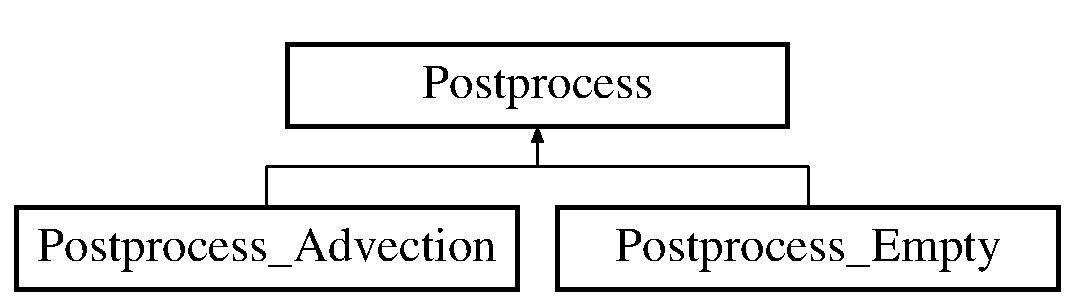
\includegraphics[height=2.000000cm]{class_postprocess}
\end{center}
\end{figure}
\subsection*{Public Member Functions}
\begin{DoxyCompactItemize}
\item 
\hyperlink{class_postprocess_ac9807b3daa36d99136f8385cc9b9a8a9}{Postprocess} (\hyperlink{class_control}{Control} $\ast$c)
\item 
virtual \hyperlink{class_postprocess_abcbe895c34b2694d2ebaa4a0b8e57ca1}{$\sim$\+Postprocess} ()
\item 
virtual void \hyperlink{class_postprocess_afd99ba74ef69d05be2f8d5bd80f0dd7a}{operator()} (\hyperlink{class_grid}{Grid} $\ast$g, const double t) const =0
\end{DoxyCompactItemize}
\subsection*{Protected Attributes}
\begin{DoxyCompactItemize}
\item 
\hyperlink{class_control}{Control} $\ast$ \hyperlink{class_postprocess_a808baccc80afb5cb6a3c28650001357a}{\+\_\+c}
\end{DoxyCompactItemize}


\subsection{Detailed Description}
Abstract class for postprocessing simulation results. 

\subsection{Constructor \& Destructor Documentation}
\index{Postprocess@{Postprocess}!Postprocess@{Postprocess}}
\index{Postprocess@{Postprocess}!Postprocess@{Postprocess}}
\subsubsection[{\texorpdfstring{Postprocess(\+Control $\ast$c)}{Postprocess(Control *c)}}]{\setlength{\rightskip}{0pt plus 5cm}Postprocess\+::\+Postprocess (
\begin{DoxyParamCaption}
\item[{{\bf Control} $\ast$}]{c}
\end{DoxyParamCaption}
)\hspace{0.3cm}{\ttfamily [inline]}}\hypertarget{class_postprocess_ac9807b3daa36d99136f8385cc9b9a8a9}{}\label{class_postprocess_ac9807b3daa36d99136f8385cc9b9a8a9}
\index{Postprocess@{Postprocess}!````~Postprocess@{$\sim$\+Postprocess}}
\index{````~Postprocess@{$\sim$\+Postprocess}!Postprocess@{Postprocess}}
\subsubsection[{\texorpdfstring{$\sim$\+Postprocess()}{~Postprocess()}}]{\setlength{\rightskip}{0pt plus 5cm}virtual Postprocess\+::$\sim$\+Postprocess (
\begin{DoxyParamCaption}
{}
\end{DoxyParamCaption}
)\hspace{0.3cm}{\ttfamily [inline]}, {\ttfamily [virtual]}}\hypertarget{class_postprocess_abcbe895c34b2694d2ebaa4a0b8e57ca1}{}\label{class_postprocess_abcbe895c34b2694d2ebaa4a0b8e57ca1}


\subsection{Member Function Documentation}
\index{Postprocess@{Postprocess}!operator()@{operator()}}
\index{operator()@{operator()}!Postprocess@{Postprocess}}
\subsubsection[{\texorpdfstring{operator()(\+Grid $\ast$g, const double t) const =0}{operator()(Grid *g, const double t) const =0}}]{\setlength{\rightskip}{0pt plus 5cm}virtual void Postprocess\+::operator() (
\begin{DoxyParamCaption}
\item[{{\bf Grid} $\ast$}]{g, }
\item[{const double}]{t}
\end{DoxyParamCaption}
) const\hspace{0.3cm}{\ttfamily [pure virtual]}}\hypertarget{class_postprocess_afd99ba74ef69d05be2f8d5bd80f0dd7a}{}\label{class_postprocess_afd99ba74ef69d05be2f8d5bd80f0dd7a}
\hyperlink{class_postprocess}{Postprocess} results 

Implemented in \hyperlink{class_postprocess___advection_a7df2f5694b2d345b8e7f19a5de18aa9d}{Postprocess\+\_\+\+Advection}, and \hyperlink{class_postprocess___empty_a4ff530ac6ee362ba6d15b4cdffc1d596}{Postprocess\+\_\+\+Empty}.



\subsection{Member Data Documentation}
\index{Postprocess@{Postprocess}!\+\_\+c@{\+\_\+c}}
\index{\+\_\+c@{\+\_\+c}!Postprocess@{Postprocess}}
\subsubsection[{\texorpdfstring{\+\_\+c}{_c}}]{\setlength{\rightskip}{0pt plus 5cm}{\bf Control}$\ast$ Postprocess\+::\+\_\+c\hspace{0.3cm}{\ttfamily [protected]}}\hypertarget{class_postprocess_a808baccc80afb5cb6a3c28650001357a}{}\label{class_postprocess_a808baccc80afb5cb6a3c28650001357a}


The documentation for this class was generated from the following file\+:\begin{DoxyCompactItemize}
\item 
/home/doberle/\+Advanced C\+F\+D/acfd/\+Code/\hyperlink{postprocess_8h}{postprocess.\+h}\end{DoxyCompactItemize}

\hypertarget{class_postprocess___advection}{}\section{Postprocess\+\_\+\+Advection Class Reference}
\label{class_postprocess___advection}\index{Postprocess\+\_\+\+Advection@{Postprocess\+\_\+\+Advection}}


Postprocessing class for the linear advection-\/diffusion equation.  




{\ttfamily \#include $<$postprocess\+\_\+advection.\+h$>$}

Inheritance diagram for Postprocess\+\_\+\+Advection\+:\begin{figure}[H]
\begin{center}
\leavevmode
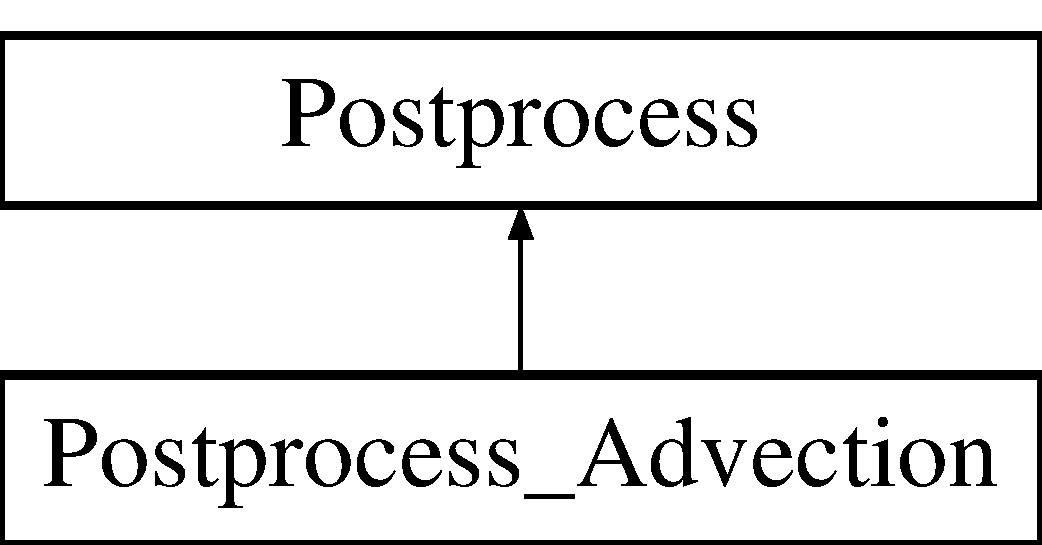
\includegraphics[height=2.000000cm]{class_postprocess___advection}
\end{center}
\end{figure}
\subsection*{Public Member Functions}
\begin{DoxyCompactItemize}
\item 
\hyperlink{class_postprocess___advection_abb7827dbb36aa66fe09f301fc2c4f385}{Postprocess\+\_\+\+Advection} (\hyperlink{class_control}{Control} $\ast$c)
\item 
\hyperlink{class_postprocess___advection_a734e3dd35af58cd20867d422d28c80fb}{$\sim$\+Postprocess\+\_\+\+Advection} ()
\item 
void \hyperlink{class_postprocess___advection_a7df2f5694b2d345b8e7f19a5de18aa9d}{operator()} (\hyperlink{class_grid}{Grid} $\ast$g, const double t) const 
\end{DoxyCompactItemize}
\subsection*{Private Member Functions}
\begin{DoxyCompactItemize}
\item 
double \hyperlink{class_postprocess___advection_a7b416da80a8ce796736910b5b3f66df4}{wrap\+\_\+to\+\_\+interval} (double value, double upper\+\_\+bound) const 
\item 
void \hyperlink{class_postprocess___advection_a261d6487e494a237784ed3b3f1597ea9}{L2\+\_\+error\+\_\+1d\+\_\+tophat} (\hyperlink{class_grid}{Grid} $\ast$g, const double t) const 
\item 
void \hyperlink{class_postprocess___advection_a2eea0ec04826ead7194cbdfc67c65adc}{L2\+\_\+error\+\_\+1d\+\_\+sin} (\hyperlink{class_grid}{Grid} $\ast$g, const double t) const 
\item 
void \hyperlink{class_postprocess___advection_abd25bc55c609922bd49cd699056290b2}{L2\+\_\+error\+\_\+2d\+\_\+tophat} (\hyperlink{class_grid}{Grid} $\ast$g, const double t) const 
\item 
void \hyperlink{class_postprocess___advection_aa5971a4fb00e3a3e8a90191280782617}{L2\+\_\+error\+\_\+2d\+\_\+sin} (\hyperlink{class_grid}{Grid} $\ast$g, const double t) const 
\end{DoxyCompactItemize}
\subsection*{Additional Inherited Members}


\subsection{Detailed Description}
Postprocessing class for the linear advection-\/diffusion equation. 

\subsection{Constructor \& Destructor Documentation}
\index{Postprocess\+\_\+\+Advection@{Postprocess\+\_\+\+Advection}!Postprocess\+\_\+\+Advection@{Postprocess\+\_\+\+Advection}}
\index{Postprocess\+\_\+\+Advection@{Postprocess\+\_\+\+Advection}!Postprocess\+\_\+\+Advection@{Postprocess\+\_\+\+Advection}}
\subsubsection[{\texorpdfstring{Postprocess\+\_\+\+Advection(\+Control $\ast$c)}{Postprocess_Advection(Control *c)}}]{\setlength{\rightskip}{0pt plus 5cm}Postprocess\+\_\+\+Advection\+::\+Postprocess\+\_\+\+Advection (
\begin{DoxyParamCaption}
\item[{{\bf Control} $\ast$}]{c}
\end{DoxyParamCaption}
)\hspace{0.3cm}{\ttfamily [inline]}}\hypertarget{class_postprocess___advection_abb7827dbb36aa66fe09f301fc2c4f385}{}\label{class_postprocess___advection_abb7827dbb36aa66fe09f301fc2c4f385}
Constructor. Uses the key \char`\"{}\+Case\+\_\+\+Postprocess\char`\"{} in the control file.
\begin{DoxyItemize}
\item 1\+: 1D postprocess
\item 2\+: 2D postprocess 
\end{DoxyItemize}\index{Postprocess\+\_\+\+Advection@{Postprocess\+\_\+\+Advection}!````~Postprocess\+\_\+\+Advection@{$\sim$\+Postprocess\+\_\+\+Advection}}
\index{````~Postprocess\+\_\+\+Advection@{$\sim$\+Postprocess\+\_\+\+Advection}!Postprocess\+\_\+\+Advection@{Postprocess\+\_\+\+Advection}}
\subsubsection[{\texorpdfstring{$\sim$\+Postprocess\+\_\+\+Advection()}{~Postprocess_Advection()}}]{\setlength{\rightskip}{0pt plus 5cm}Postprocess\+\_\+\+Advection\+::$\sim$\+Postprocess\+\_\+\+Advection (
\begin{DoxyParamCaption}
{}
\end{DoxyParamCaption}
)\hspace{0.3cm}{\ttfamily [inline]}}\hypertarget{class_postprocess___advection_a734e3dd35af58cd20867d422d28c80fb}{}\label{class_postprocess___advection_a734e3dd35af58cd20867d422d28c80fb}


\subsection{Member Function Documentation}
\index{Postprocess\+\_\+\+Advection@{Postprocess\+\_\+\+Advection}!L2\+\_\+error\+\_\+1d\+\_\+sin@{L2\+\_\+error\+\_\+1d\+\_\+sin}}
\index{L2\+\_\+error\+\_\+1d\+\_\+sin@{L2\+\_\+error\+\_\+1d\+\_\+sin}!Postprocess\+\_\+\+Advection@{Postprocess\+\_\+\+Advection}}
\subsubsection[{\texorpdfstring{L2\+\_\+error\+\_\+1d\+\_\+sin(\+Grid $\ast$g, const double t) const }{L2_error_1d_sin(Grid *g, const double t) const }}]{\setlength{\rightskip}{0pt plus 5cm}void Postprocess\+\_\+\+Advection\+::\+L2\+\_\+error\+\_\+1d\+\_\+sin (
\begin{DoxyParamCaption}
\item[{{\bf Grid} $\ast$}]{g, }
\item[{const double}]{t}
\end{DoxyParamCaption}
) const\hspace{0.3cm}{\ttfamily [private]}}\hypertarget{class_postprocess___advection_a2eea0ec04826ead7194cbdfc67c65adc}{}\label{class_postprocess___advection_a2eea0ec04826ead7194cbdfc67c65adc}
\index{Postprocess\+\_\+\+Advection@{Postprocess\+\_\+\+Advection}!L2\+\_\+error\+\_\+1d\+\_\+tophat@{L2\+\_\+error\+\_\+1d\+\_\+tophat}}
\index{L2\+\_\+error\+\_\+1d\+\_\+tophat@{L2\+\_\+error\+\_\+1d\+\_\+tophat}!Postprocess\+\_\+\+Advection@{Postprocess\+\_\+\+Advection}}
\subsubsection[{\texorpdfstring{L2\+\_\+error\+\_\+1d\+\_\+tophat(\+Grid $\ast$g, const double t) const }{L2_error_1d_tophat(Grid *g, const double t) const }}]{\setlength{\rightskip}{0pt plus 5cm}void Postprocess\+\_\+\+Advection\+::\+L2\+\_\+error\+\_\+1d\+\_\+tophat (
\begin{DoxyParamCaption}
\item[{{\bf Grid} $\ast$}]{g, }
\item[{const double}]{t}
\end{DoxyParamCaption}
) const\hspace{0.3cm}{\ttfamily [private]}}\hypertarget{class_postprocess___advection_a261d6487e494a237784ed3b3f1597ea9}{}\label{class_postprocess___advection_a261d6487e494a237784ed3b3f1597ea9}
\index{Postprocess\+\_\+\+Advection@{Postprocess\+\_\+\+Advection}!L2\+\_\+error\+\_\+2d\+\_\+sin@{L2\+\_\+error\+\_\+2d\+\_\+sin}}
\index{L2\+\_\+error\+\_\+2d\+\_\+sin@{L2\+\_\+error\+\_\+2d\+\_\+sin}!Postprocess\+\_\+\+Advection@{Postprocess\+\_\+\+Advection}}
\subsubsection[{\texorpdfstring{L2\+\_\+error\+\_\+2d\+\_\+sin(\+Grid $\ast$g, const double t) const }{L2_error_2d_sin(Grid *g, const double t) const }}]{\setlength{\rightskip}{0pt plus 5cm}void Postprocess\+\_\+\+Advection\+::\+L2\+\_\+error\+\_\+2d\+\_\+sin (
\begin{DoxyParamCaption}
\item[{{\bf Grid} $\ast$}]{g, }
\item[{const double}]{t}
\end{DoxyParamCaption}
) const\hspace{0.3cm}{\ttfamily [private]}}\hypertarget{class_postprocess___advection_aa5971a4fb00e3a3e8a90191280782617}{}\label{class_postprocess___advection_aa5971a4fb00e3a3e8a90191280782617}
\index{Postprocess\+\_\+\+Advection@{Postprocess\+\_\+\+Advection}!L2\+\_\+error\+\_\+2d\+\_\+tophat@{L2\+\_\+error\+\_\+2d\+\_\+tophat}}
\index{L2\+\_\+error\+\_\+2d\+\_\+tophat@{L2\+\_\+error\+\_\+2d\+\_\+tophat}!Postprocess\+\_\+\+Advection@{Postprocess\+\_\+\+Advection}}
\subsubsection[{\texorpdfstring{L2\+\_\+error\+\_\+2d\+\_\+tophat(\+Grid $\ast$g, const double t) const }{L2_error_2d_tophat(Grid *g, const double t) const }}]{\setlength{\rightskip}{0pt plus 5cm}void Postprocess\+\_\+\+Advection\+::\+L2\+\_\+error\+\_\+2d\+\_\+tophat (
\begin{DoxyParamCaption}
\item[{{\bf Grid} $\ast$}]{g, }
\item[{const double}]{t}
\end{DoxyParamCaption}
) const\hspace{0.3cm}{\ttfamily [private]}}\hypertarget{class_postprocess___advection_abd25bc55c609922bd49cd699056290b2}{}\label{class_postprocess___advection_abd25bc55c609922bd49cd699056290b2}
\index{Postprocess\+\_\+\+Advection@{Postprocess\+\_\+\+Advection}!operator()@{operator()}}
\index{operator()@{operator()}!Postprocess\+\_\+\+Advection@{Postprocess\+\_\+\+Advection}}
\subsubsection[{\texorpdfstring{operator()(\+Grid $\ast$g, const double t) const }{operator()(Grid *g, const double t) const }}]{\setlength{\rightskip}{0pt plus 5cm}void Postprocess\+\_\+\+Advection\+::operator() (
\begin{DoxyParamCaption}
\item[{{\bf Grid} $\ast$}]{g, }
\item[{const double}]{t}
\end{DoxyParamCaption}
) const\hspace{0.3cm}{\ttfamily [inline]}, {\ttfamily [virtual]}}\hypertarget{class_postprocess___advection_a7df2f5694b2d345b8e7f19a5de18aa9d}{}\label{class_postprocess___advection_a7df2f5694b2d345b8e7f19a5de18aa9d}
Compute the L2 error of the numerical solution. Currently, this only works without diffusion (mu = 0). Uses the key \char`\"{}\+Case\+\_\+\+Init\char`\"{} to choose the analytical solution to compare against. 

Implements \hyperlink{class_postprocess_afd99ba74ef69d05be2f8d5bd80f0dd7a}{Postprocess}.

\index{Postprocess\+\_\+\+Advection@{Postprocess\+\_\+\+Advection}!wrap\+\_\+to\+\_\+interval@{wrap\+\_\+to\+\_\+interval}}
\index{wrap\+\_\+to\+\_\+interval@{wrap\+\_\+to\+\_\+interval}!Postprocess\+\_\+\+Advection@{Postprocess\+\_\+\+Advection}}
\subsubsection[{\texorpdfstring{wrap\+\_\+to\+\_\+interval(double value, double upper\+\_\+bound) const }{wrap_to_interval(double value, double upper_bound) const }}]{\setlength{\rightskip}{0pt plus 5cm}double Postprocess\+\_\+\+Advection\+::wrap\+\_\+to\+\_\+interval (
\begin{DoxyParamCaption}
\item[{double}]{value, }
\item[{double}]{upper\+\_\+bound}
\end{DoxyParamCaption}
) const\hspace{0.3cm}{\ttfamily [inline]}, {\ttfamily [private]}}\hypertarget{class_postprocess___advection_a7b416da80a8ce796736910b5b3f66df4}{}\label{class_postprocess___advection_a7b416da80a8ce796736910b5b3f66df4}
Wrap a given value to the interval \mbox{[}0, upper\+\_\+bound). 

The documentation for this class was generated from the following files\+:\begin{DoxyCompactItemize}
\item 
/home/doberle/\+Advanced C\+F\+D/acfd/\+Code/\hyperlink{postprocess__advection_8h}{postprocess\+\_\+advection.\+h}\item 
/home/doberle/\+Advanced C\+F\+D/acfd/\+Code/\hyperlink{postprocess__advection_8cpp}{postprocess\+\_\+advection.\+cpp}\end{DoxyCompactItemize}

\hypertarget{class_postprocess___empty}{}\section{Postprocess\+\_\+\+Empty Class Reference}
\label{class_postprocess___empty}\index{Postprocess\+\_\+\+Empty@{Postprocess\+\_\+\+Empty}}


Empty postprocessing class (does nothing)  




{\ttfamily \#include $<$postprocess\+\_\+empty.\+h$>$}

Inheritance diagram for Postprocess\+\_\+\+Empty\+:\begin{figure}[H]
\begin{center}
\leavevmode
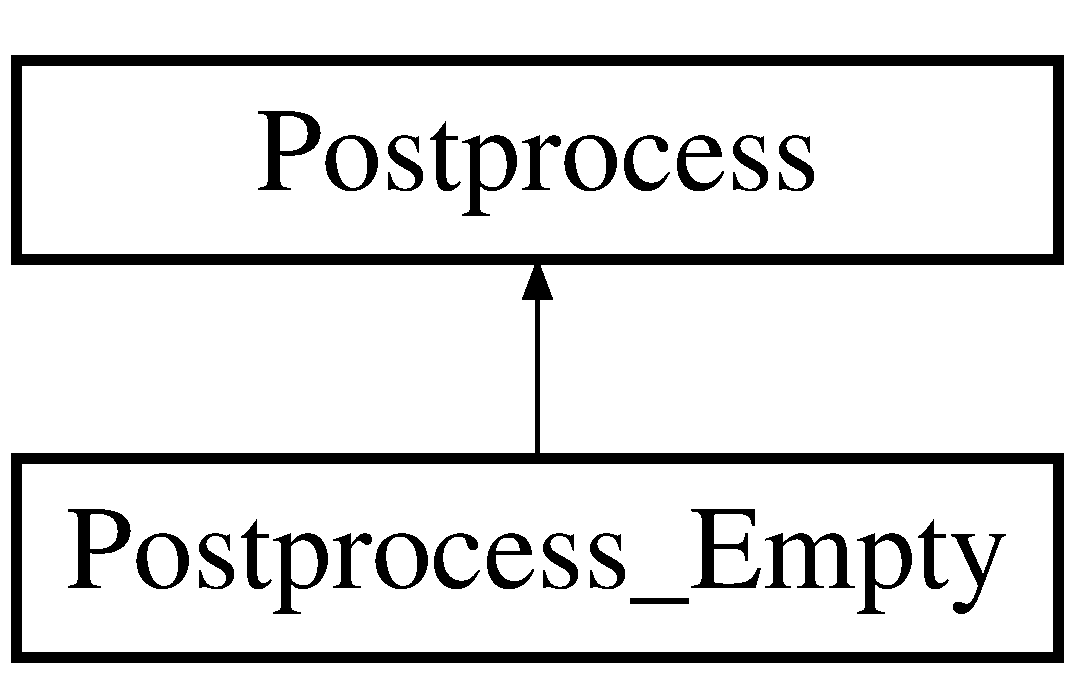
\includegraphics[height=2.000000cm]{class_postprocess___empty}
\end{center}
\end{figure}
\subsection*{Public Member Functions}
\begin{DoxyCompactItemize}
\item 
\hyperlink{class_postprocess___empty_aa05a5aab05e64ff937ce844e3b08e17a}{Postprocess\+\_\+\+Empty} (\hyperlink{class_control}{Control} $\ast$c)
\item 
virtual \hyperlink{class_postprocess___empty_a44b647468fdde2620bc9e047f50076ab}{$\sim$\+Postprocess\+\_\+\+Empty} ()
\item 
virtual void \hyperlink{class_postprocess___empty_a4ff530ac6ee362ba6d15b4cdffc1d596}{operator()} (\hyperlink{class_grid}{Grid} $\ast$g, const double t) const 
\end{DoxyCompactItemize}
\subsection*{Additional Inherited Members}


\subsection{Detailed Description}
Empty postprocessing class (does nothing) 

\subsection{Constructor \& Destructor Documentation}
\index{Postprocess\+\_\+\+Empty@{Postprocess\+\_\+\+Empty}!Postprocess\+\_\+\+Empty@{Postprocess\+\_\+\+Empty}}
\index{Postprocess\+\_\+\+Empty@{Postprocess\+\_\+\+Empty}!Postprocess\+\_\+\+Empty@{Postprocess\+\_\+\+Empty}}
\subsubsection[{\texorpdfstring{Postprocess\+\_\+\+Empty(\+Control $\ast$c)}{Postprocess_Empty(Control *c)}}]{\setlength{\rightskip}{0pt plus 5cm}Postprocess\+\_\+\+Empty\+::\+Postprocess\+\_\+\+Empty (
\begin{DoxyParamCaption}
\item[{{\bf Control} $\ast$}]{c}
\end{DoxyParamCaption}
)\hspace{0.3cm}{\ttfamily [inline]}}\hypertarget{class_postprocess___empty_aa05a5aab05e64ff937ce844e3b08e17a}{}\label{class_postprocess___empty_aa05a5aab05e64ff937ce844e3b08e17a}
\index{Postprocess\+\_\+\+Empty@{Postprocess\+\_\+\+Empty}!````~Postprocess\+\_\+\+Empty@{$\sim$\+Postprocess\+\_\+\+Empty}}
\index{````~Postprocess\+\_\+\+Empty@{$\sim$\+Postprocess\+\_\+\+Empty}!Postprocess\+\_\+\+Empty@{Postprocess\+\_\+\+Empty}}
\subsubsection[{\texorpdfstring{$\sim$\+Postprocess\+\_\+\+Empty()}{~Postprocess_Empty()}}]{\setlength{\rightskip}{0pt plus 5cm}virtual Postprocess\+\_\+\+Empty\+::$\sim$\+Postprocess\+\_\+\+Empty (
\begin{DoxyParamCaption}
{}
\end{DoxyParamCaption}
)\hspace{0.3cm}{\ttfamily [inline]}, {\ttfamily [virtual]}}\hypertarget{class_postprocess___empty_a44b647468fdde2620bc9e047f50076ab}{}\label{class_postprocess___empty_a44b647468fdde2620bc9e047f50076ab}


\subsection{Member Function Documentation}
\index{Postprocess\+\_\+\+Empty@{Postprocess\+\_\+\+Empty}!operator()@{operator()}}
\index{operator()@{operator()}!Postprocess\+\_\+\+Empty@{Postprocess\+\_\+\+Empty}}
\subsubsection[{\texorpdfstring{operator()(\+Grid $\ast$g, const double t) const }{operator()(Grid *g, const double t) const }}]{\setlength{\rightskip}{0pt plus 5cm}virtual void Postprocess\+\_\+\+Empty\+::operator() (
\begin{DoxyParamCaption}
\item[{{\bf Grid} $\ast$}]{g, }
\item[{const double}]{t}
\end{DoxyParamCaption}
) const\hspace{0.3cm}{\ttfamily [inline]}, {\ttfamily [virtual]}}\hypertarget{class_postprocess___empty_a4ff530ac6ee362ba6d15b4cdffc1d596}{}\label{class_postprocess___empty_a4ff530ac6ee362ba6d15b4cdffc1d596}
Empty postprocess (do nothing) 

Implements \hyperlink{class_postprocess_afd99ba74ef69d05be2f8d5bd80f0dd7a}{Postprocess}.



The documentation for this class was generated from the following file\+:\begin{DoxyCompactItemize}
\item 
/home/doberle/\+Advanced C\+F\+D/acfd/\+Code/\hyperlink{postprocess__empty_8h}{postprocess\+\_\+empty.\+h}\end{DoxyCompactItemize}

\hypertarget{class_setup}{}\section{Setup Class Reference}
\label{class_setup}\index{Setup@{Setup}}


Class for the simulation setup.  




{\ttfamily \#include $<$setup.\+h$>$}

Inheritance diagram for Setup\+:\begin{figure}[H]
\begin{center}
\leavevmode
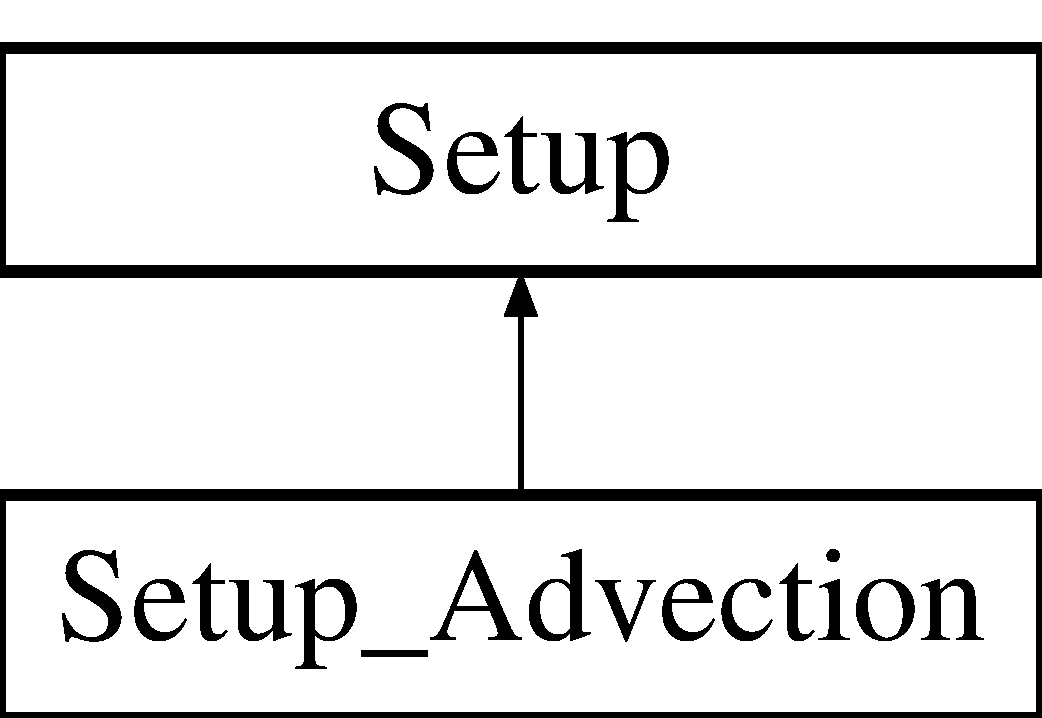
\includegraphics[height=2.000000cm]{class_setup}
\end{center}
\end{figure}
\subsection*{Public Member Functions}
\begin{DoxyCompactItemize}
\item 
virtual \hyperlink{class_setup_aa402859a81d394a981849b4b9b1605a4}{$\sim$\+Setup} ()
\item 
virtual void \hyperlink{class_setup_a9f0d9baa17df8ae6876f3041788c559a}{refresh} ()
\end{DoxyCompactItemize}
\subsection*{Protected Attributes}
\begin{DoxyCompactItemize}
\item 
\hyperlink{class_control}{Control} $\ast$ \hyperlink{class_setup_a9b66656cfab0fbe2e17582cd3d9bc392}{\+\_\+c}
\item 
\hyperlink{class_grid}{Grid} $\ast$ \hyperlink{class_setup_a2812ab3c7f7322e9f77e4c4d43053655}{\+\_\+g}
\item 
\hyperlink{class_time}{Time} $\ast$ \hyperlink{class_setup_acbbdb0a7312ce4dd45a64a200d780c3d}{\+\_\+t}
\item 
\hyperlink{class_init}{Init} $\ast$ \hyperlink{class_setup_afc816a430e9d93f357229d9525f686b8}{\+\_\+i}
\item 
\hyperlink{class_boundary}{Boundary} $\ast$ \hyperlink{class_setup_ae76b77049e072bcd37017a5f5c5ebcec}{\+\_\+b}
\item 
\hyperlink{class_fluxes}{Fluxes} $\ast$ \hyperlink{class_setup_acd47ea266d609c5fbef77579608308a5}{\+\_\+f}
\item 
\hyperlink{class_source}{Source} $\ast$ \hyperlink{class_setup_a0b2e5fd96ef68ea898700ead61d27973}{\+\_\+q}
\item 
\hyperlink{class_update}{Update} $\ast$ \hyperlink{class_setup_a873ce4c87704142ce98b6cc0dfd779e7}{\+\_\+u}
\item 
\hyperlink{class_plot}{Plot} $\ast$ \hyperlink{class_setup_ad2cca0e00dff58e8f63a0ec3b652cab7}{\+\_\+p}
\item 
\hyperlink{class_postprocess}{Postprocess} $\ast$ \hyperlink{class_setup_adc487395b8e8221d9b8f0ba0b29d2540}{\+\_\+pp}
\end{DoxyCompactItemize}


\subsection{Detailed Description}
Class for the simulation setup. 

This class allocates and deletes all required pointers. Classes derived from \hyperlink{class_setup}{Setup} need to allocate objects of type \hyperlink{class_control}{Control}, \hyperlink{class_grid}{Grid}, \hyperlink{class_time}{Time}, \hyperlink{class_init}{Init}, \hyperlink{class_boundary}{Boundary}, \hyperlink{class_fluxes}{Fluxes}, \hyperlink{class_source}{Source}, \hyperlink{class_update}{Update} and \hyperlink{class_plot}{Plot}.

This class is not abstract but no object should be instantiated since there is only a default constructor that does nothing. 

\subsection{Constructor \& Destructor Documentation}
\index{Setup@{Setup}!````~Setup@{$\sim$\+Setup}}
\index{````~Setup@{$\sim$\+Setup}!Setup@{Setup}}
\subsubsection[{\texorpdfstring{$\sim$\+Setup()}{~Setup()}}]{\setlength{\rightskip}{0pt plus 5cm}virtual Setup\+::$\sim$\+Setup (
\begin{DoxyParamCaption}
{}
\end{DoxyParamCaption}
)\hspace{0.3cm}{\ttfamily [inline]}, {\ttfamily [virtual]}}\hypertarget{class_setup_aa402859a81d394a981849b4b9b1605a4}{}\label{class_setup_aa402859a81d394a981849b4b9b1605a4}
Destructor that deletes all pointers 

\subsection{Member Function Documentation}
\index{Setup@{Setup}!refresh@{refresh}}
\index{refresh@{refresh}!Setup@{Setup}}
\subsubsection[{\texorpdfstring{refresh()}{refresh()}}]{\setlength{\rightskip}{0pt plus 5cm}virtual void Setup\+::refresh (
\begin{DoxyParamCaption}
{}
\end{DoxyParamCaption}
)\hspace{0.3cm}{\ttfamily [inline]}, {\ttfamily [virtual]}}\hypertarget{class_setup_a9f0d9baa17df8ae6876f3041788c559a}{}\label{class_setup_a9f0d9baa17df8ae6876f3041788c559a}
Reread the entries \char`\"{}dt\char`\"{}, \char`\"{}nout\char`\"{} and \char`\"{}nt\char`\"{} from the control file 

\subsection{Member Data Documentation}
\index{Setup@{Setup}!\+\_\+b@{\+\_\+b}}
\index{\+\_\+b@{\+\_\+b}!Setup@{Setup}}
\subsubsection[{\texorpdfstring{\+\_\+b}{_b}}]{\setlength{\rightskip}{0pt plus 5cm}{\bf Boundary}$\ast$ Setup\+::\+\_\+b\hspace{0.3cm}{\ttfamily [protected]}}\hypertarget{class_setup_ae76b77049e072bcd37017a5f5c5ebcec}{}\label{class_setup_ae76b77049e072bcd37017a5f5c5ebcec}
\index{Setup@{Setup}!\+\_\+c@{\+\_\+c}}
\index{\+\_\+c@{\+\_\+c}!Setup@{Setup}}
\subsubsection[{\texorpdfstring{\+\_\+c}{_c}}]{\setlength{\rightskip}{0pt plus 5cm}{\bf Control}$\ast$ Setup\+::\+\_\+c\hspace{0.3cm}{\ttfamily [protected]}}\hypertarget{class_setup_a9b66656cfab0fbe2e17582cd3d9bc392}{}\label{class_setup_a9b66656cfab0fbe2e17582cd3d9bc392}
\index{Setup@{Setup}!\+\_\+f@{\+\_\+f}}
\index{\+\_\+f@{\+\_\+f}!Setup@{Setup}}
\subsubsection[{\texorpdfstring{\+\_\+f}{_f}}]{\setlength{\rightskip}{0pt plus 5cm}{\bf Fluxes}$\ast$ Setup\+::\+\_\+f\hspace{0.3cm}{\ttfamily [protected]}}\hypertarget{class_setup_acd47ea266d609c5fbef77579608308a5}{}\label{class_setup_acd47ea266d609c5fbef77579608308a5}
\index{Setup@{Setup}!\+\_\+g@{\+\_\+g}}
\index{\+\_\+g@{\+\_\+g}!Setup@{Setup}}
\subsubsection[{\texorpdfstring{\+\_\+g}{_g}}]{\setlength{\rightskip}{0pt plus 5cm}{\bf Grid}$\ast$ Setup\+::\+\_\+g\hspace{0.3cm}{\ttfamily [protected]}}\hypertarget{class_setup_a2812ab3c7f7322e9f77e4c4d43053655}{}\label{class_setup_a2812ab3c7f7322e9f77e4c4d43053655}
\index{Setup@{Setup}!\+\_\+i@{\+\_\+i}}
\index{\+\_\+i@{\+\_\+i}!Setup@{Setup}}
\subsubsection[{\texorpdfstring{\+\_\+i}{_i}}]{\setlength{\rightskip}{0pt plus 5cm}{\bf Init}$\ast$ Setup\+::\+\_\+i\hspace{0.3cm}{\ttfamily [protected]}}\hypertarget{class_setup_afc816a430e9d93f357229d9525f686b8}{}\label{class_setup_afc816a430e9d93f357229d9525f686b8}
\index{Setup@{Setup}!\+\_\+p@{\+\_\+p}}
\index{\+\_\+p@{\+\_\+p}!Setup@{Setup}}
\subsubsection[{\texorpdfstring{\+\_\+p}{_p}}]{\setlength{\rightskip}{0pt plus 5cm}{\bf Plot}$\ast$ Setup\+::\+\_\+p\hspace{0.3cm}{\ttfamily [protected]}}\hypertarget{class_setup_ad2cca0e00dff58e8f63a0ec3b652cab7}{}\label{class_setup_ad2cca0e00dff58e8f63a0ec3b652cab7}
\index{Setup@{Setup}!\+\_\+pp@{\+\_\+pp}}
\index{\+\_\+pp@{\+\_\+pp}!Setup@{Setup}}
\subsubsection[{\texorpdfstring{\+\_\+pp}{_pp}}]{\setlength{\rightskip}{0pt plus 5cm}{\bf Postprocess}$\ast$ Setup\+::\+\_\+pp\hspace{0.3cm}{\ttfamily [protected]}}\hypertarget{class_setup_adc487395b8e8221d9b8f0ba0b29d2540}{}\label{class_setup_adc487395b8e8221d9b8f0ba0b29d2540}
\index{Setup@{Setup}!\+\_\+q@{\+\_\+q}}
\index{\+\_\+q@{\+\_\+q}!Setup@{Setup}}
\subsubsection[{\texorpdfstring{\+\_\+q}{_q}}]{\setlength{\rightskip}{0pt plus 5cm}{\bf Source}$\ast$ Setup\+::\+\_\+q\hspace{0.3cm}{\ttfamily [protected]}}\hypertarget{class_setup_a0b2e5fd96ef68ea898700ead61d27973}{}\label{class_setup_a0b2e5fd96ef68ea898700ead61d27973}
\index{Setup@{Setup}!\+\_\+t@{\+\_\+t}}
\index{\+\_\+t@{\+\_\+t}!Setup@{Setup}}
\subsubsection[{\texorpdfstring{\+\_\+t}{_t}}]{\setlength{\rightskip}{0pt plus 5cm}{\bf Time}$\ast$ Setup\+::\+\_\+t\hspace{0.3cm}{\ttfamily [protected]}}\hypertarget{class_setup_acbbdb0a7312ce4dd45a64a200d780c3d}{}\label{class_setup_acbbdb0a7312ce4dd45a64a200d780c3d}
\index{Setup@{Setup}!\+\_\+u@{\+\_\+u}}
\index{\+\_\+u@{\+\_\+u}!Setup@{Setup}}
\subsubsection[{\texorpdfstring{\+\_\+u}{_u}}]{\setlength{\rightskip}{0pt plus 5cm}{\bf Update}$\ast$ Setup\+::\+\_\+u\hspace{0.3cm}{\ttfamily [protected]}}\hypertarget{class_setup_a873ce4c87704142ce98b6cc0dfd779e7}{}\label{class_setup_a873ce4c87704142ce98b6cc0dfd779e7}


The documentation for this class was generated from the following file\+:\begin{DoxyCompactItemize}
\item 
/home/doberle/\+Advanced C\+F\+D/acfd/\+Code/\hyperlink{setup_8h}{setup.\+h}\end{DoxyCompactItemize}

\hypertarget{class_setup___advection}{}\section{Setup\+\_\+\+Advection Class Reference}
\label{class_setup___advection}\index{Setup\+\_\+\+Advection@{Setup\+\_\+\+Advection}}


Simulation setup for the linear advection-\/diffusion equation.  




{\ttfamily \#include $<$setup\+\_\+advection.\+h$>$}

Inheritance diagram for Setup\+\_\+\+Advection\+:\begin{figure}[H]
\begin{center}
\leavevmode
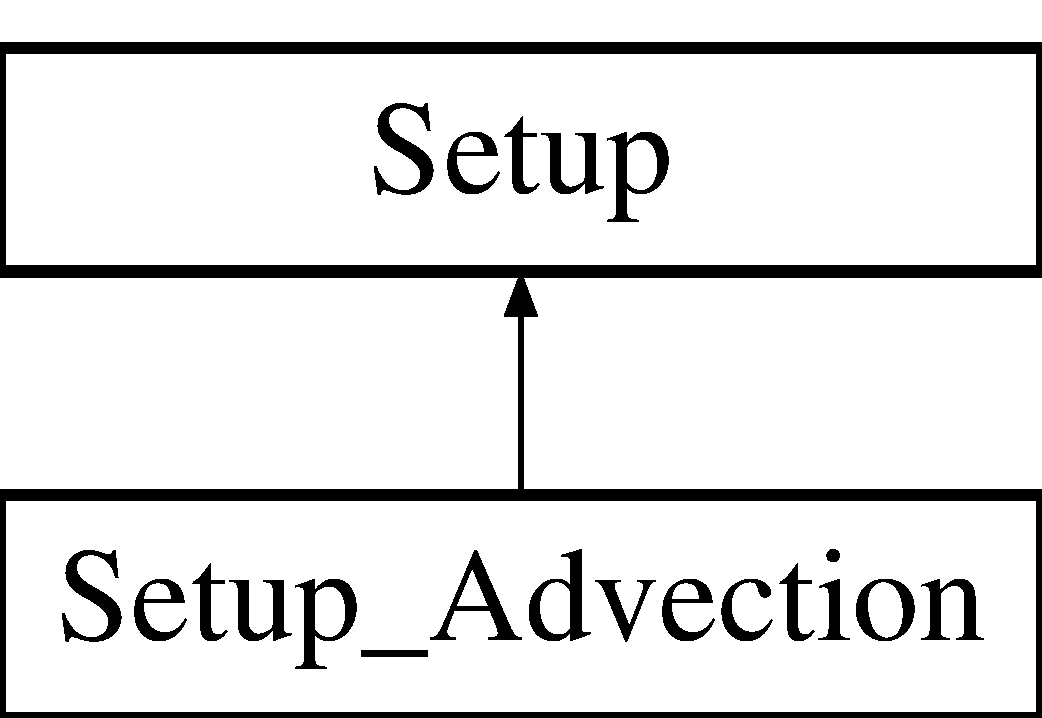
\includegraphics[height=2.000000cm]{class_setup___advection}
\end{center}
\end{figure}
\subsection*{Public Member Functions}
\begin{DoxyCompactItemize}
\item 
\hyperlink{class_setup___advection_aa02d5e7d008f8860a6c54dff04011212}{Setup\+\_\+\+Advection} (\hyperlink{class_control}{Control} $\ast$$\ast$c, \hyperlink{class_time}{Time} $\ast$$\ast$t, \hyperlink{class_grid}{Grid} $\ast$$\ast$g, \hyperlink{class_init}{Init} $\ast$$\ast$i, \hyperlink{class_boundary}{Boundary} $\ast$$\ast$b, \hyperlink{class_fluxes}{Fluxes} $\ast$$\ast$f, \hyperlink{class_source}{Source} $\ast$$\ast$q, \hyperlink{class_update}{Update} $\ast$$\ast$u, \hyperlink{class_plot}{Plot} $\ast$$\ast$p, \hyperlink{class_postprocess}{Postprocess} $\ast$$\ast$pp)
\end{DoxyCompactItemize}
\subsection*{Additional Inherited Members}


\subsection{Detailed Description}
Simulation setup for the linear advection-\/diffusion equation. 

\subsection{Constructor \& Destructor Documentation}
\index{Setup\+\_\+\+Advection@{Setup\+\_\+\+Advection}!Setup\+\_\+\+Advection@{Setup\+\_\+\+Advection}}
\index{Setup\+\_\+\+Advection@{Setup\+\_\+\+Advection}!Setup\+\_\+\+Advection@{Setup\+\_\+\+Advection}}
\subsubsection[{\texorpdfstring{Setup\+\_\+\+Advection(\+Control $\ast$$\ast$c, Time $\ast$$\ast$t, Grid $\ast$$\ast$g, Init $\ast$$\ast$i, Boundary $\ast$$\ast$b, Fluxes $\ast$$\ast$f, Source $\ast$$\ast$q, Update $\ast$$\ast$u, Plot $\ast$$\ast$p, Postprocess $\ast$$\ast$pp)}{Setup_Advection(Control **c, Time **t, Grid **g, Init **i, Boundary **b, Fluxes **f, Source **q, Update **u, Plot **p, Postprocess **pp)}}]{\setlength{\rightskip}{0pt plus 5cm}Setup\+\_\+\+Advection\+::\+Setup\+\_\+\+Advection (
\begin{DoxyParamCaption}
\item[{{\bf Control} $\ast$$\ast$}]{c, }
\item[{{\bf Time} $\ast$$\ast$}]{t, }
\item[{{\bf Grid} $\ast$$\ast$}]{g, }
\item[{{\bf Init} $\ast$$\ast$}]{i, }
\item[{{\bf Boundary} $\ast$$\ast$}]{b, }
\item[{{\bf Fluxes} $\ast$$\ast$}]{f, }
\item[{{\bf Source} $\ast$$\ast$}]{q, }
\item[{{\bf Update} $\ast$$\ast$}]{u, }
\item[{{\bf Plot} $\ast$$\ast$}]{p, }
\item[{{\bf Postprocess} $\ast$$\ast$}]{pp}
\end{DoxyParamCaption}
)\hspace{0.3cm}{\ttfamily [inline]}}\hypertarget{class_setup___advection_aa02d5e7d008f8860a6c54dff04011212}{}\label{class_setup___advection_aa02d5e7d008f8860a6c54dff04011212}
Constructor that allocates all member pointers

The control file \char`\"{}advect.\+ctr\char`\"{} is used for the setup.

The arguments are passed as double pointers (of type Class$\ast$$\ast$) and the corresponding pointers (of type Class$\ast$) are allocated in this constructor. Therefore, the caller has access to all created objects. 

The documentation for this class was generated from the following file\+:\begin{DoxyCompactItemize}
\item 
/home/doberle/\+Advanced C\+F\+D/acfd/\+Code/\hyperlink{setup__advection_8h}{setup\+\_\+advection.\+h}\end{DoxyCompactItemize}

\hypertarget{class_source}{}\section{Source Class Reference}
\label{class_source}\index{Source@{Source}}


Abstract class for a source term that is applied to a \hyperlink{class_grid}{Grid} object.  




{\ttfamily \#include $<$source.\+h$>$}

Inheritance diagram for Source\+:\begin{figure}[H]
\begin{center}
\leavevmode
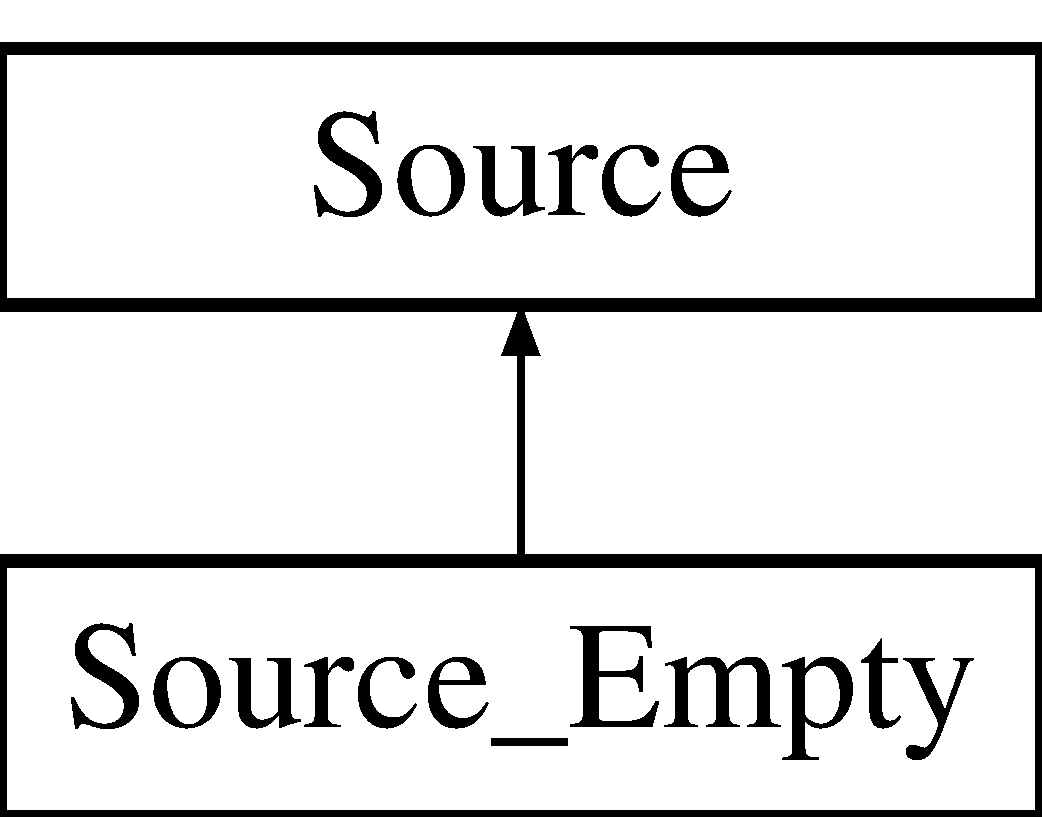
\includegraphics[height=2.000000cm]{class_source}
\end{center}
\end{figure}
\subsection*{Public Member Functions}
\begin{DoxyCompactItemize}
\item 
\hyperlink{class_source_a380f9873aa65dc95aa96703b450e74be}{Source} (\hyperlink{class_grid}{Grid} $\ast$g)
\item 
virtual \hyperlink{class_source_ad78297e3d514281fedd1d727e80bf158}{$\sim$\+Source} ()
\item 
virtual void \hyperlink{class_source_a2e3a7315e7621a6b8a3c931f7899d572}{operator()} (\hyperlink{class_grid}{Grid} $\ast$g) const =0
\end{DoxyCompactItemize}


\subsection{Detailed Description}
Abstract class for a source term that is applied to a \hyperlink{class_grid}{Grid} object. 

\subsection{Constructor \& Destructor Documentation}
\index{Source@{Source}!Source@{Source}}
\index{Source@{Source}!Source@{Source}}
\subsubsection[{\texorpdfstring{Source(\+Grid $\ast$g)}{Source(Grid *g)}}]{\setlength{\rightskip}{0pt plus 5cm}Source\+::\+Source (
\begin{DoxyParamCaption}
\item[{{\bf Grid} $\ast$}]{g}
\end{DoxyParamCaption}
)\hspace{0.3cm}{\ttfamily [inline]}}\hypertarget{class_source_a380f9873aa65dc95aa96703b450e74be}{}\label{class_source_a380f9873aa65dc95aa96703b450e74be}
Constructor that sets the source term to zero \index{Source@{Source}!````~Source@{$\sim$\+Source}}
\index{````~Source@{$\sim$\+Source}!Source@{Source}}
\subsubsection[{\texorpdfstring{$\sim$\+Source()}{~Source()}}]{\setlength{\rightskip}{0pt plus 5cm}virtual Source\+::$\sim$\+Source (
\begin{DoxyParamCaption}
{}
\end{DoxyParamCaption}
)\hspace{0.3cm}{\ttfamily [inline]}, {\ttfamily [virtual]}}\hypertarget{class_source_ad78297e3d514281fedd1d727e80bf158}{}\label{class_source_ad78297e3d514281fedd1d727e80bf158}


\subsection{Member Function Documentation}
\index{Source@{Source}!operator()@{operator()}}
\index{operator()@{operator()}!Source@{Source}}
\subsubsection[{\texorpdfstring{operator()(\+Grid $\ast$g) const =0}{operator()(Grid *g) const =0}}]{\setlength{\rightskip}{0pt plus 5cm}virtual void Source\+::operator() (
\begin{DoxyParamCaption}
\item[{{\bf Grid} $\ast$}]{g}
\end{DoxyParamCaption}
) const\hspace{0.3cm}{\ttfamily [pure virtual]}}\hypertarget{class_source_a2e3a7315e7621a6b8a3c931f7899d572}{}\label{class_source_a2e3a7315e7621a6b8a3c931f7899d572}
Set the source term value in the \hyperlink{class_grid}{Grid} object 

Implemented in \hyperlink{class_source___empty_ae553d6a7e2085934d79926b318f5ab61}{Source\+\_\+\+Empty}.



The documentation for this class was generated from the following file\+:\begin{DoxyCompactItemize}
\item 
/home/doberle/\+Advanced C\+F\+D/acfd/\+Code/\hyperlink{source_8h}{source.\+h}\end{DoxyCompactItemize}

\hypertarget{class_source___empty}{}\section{Source\+\_\+\+Empty Class Reference}
\label{class_source___empty}\index{Source\+\_\+\+Empty@{Source\+\_\+\+Empty}}


Empty source, i.\+e., the source term equals zero.  




{\ttfamily \#include $<$source\+\_\+empty.\+h$>$}

Inheritance diagram for Source\+\_\+\+Empty\+:\begin{figure}[H]
\begin{center}
\leavevmode
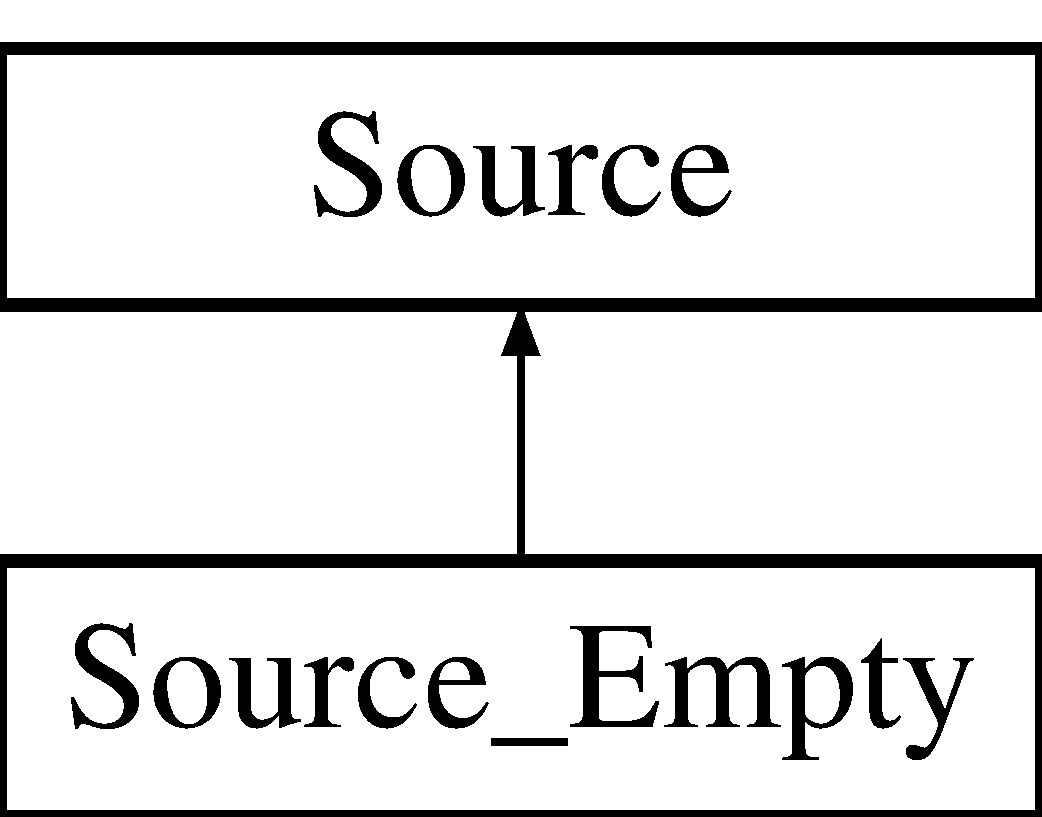
\includegraphics[height=2.000000cm]{class_source___empty}
\end{center}
\end{figure}
\subsection*{Public Member Functions}
\begin{DoxyCompactItemize}
\item 
\hyperlink{class_source___empty_ae114543d9591e98a0ed9d343469a7628}{Source\+\_\+\+Empty} (\hyperlink{class_grid}{Grid} $\ast$g)
\item 
void \hyperlink{class_source___empty_ae553d6a7e2085934d79926b318f5ab61}{operator()} (\hyperlink{class_grid}{Grid} $\ast$g) const 
\end{DoxyCompactItemize}


\subsection{Detailed Description}
Empty source, i.\+e., the source term equals zero. 

\subsection{Constructor \& Destructor Documentation}
\index{Source\+\_\+\+Empty@{Source\+\_\+\+Empty}!Source\+\_\+\+Empty@{Source\+\_\+\+Empty}}
\index{Source\+\_\+\+Empty@{Source\+\_\+\+Empty}!Source\+\_\+\+Empty@{Source\+\_\+\+Empty}}
\subsubsection[{\texorpdfstring{Source\+\_\+\+Empty(\+Grid $\ast$g)}{Source_Empty(Grid *g)}}]{\setlength{\rightskip}{0pt plus 5cm}Source\+\_\+\+Empty\+::\+Source\+\_\+\+Empty (
\begin{DoxyParamCaption}
\item[{{\bf Grid} $\ast$}]{g}
\end{DoxyParamCaption}
)\hspace{0.3cm}{\ttfamily [inline]}}\hypertarget{class_source___empty_ae114543d9591e98a0ed9d343469a7628}{}\label{class_source___empty_ae114543d9591e98a0ed9d343469a7628}


\subsection{Member Function Documentation}
\index{Source\+\_\+\+Empty@{Source\+\_\+\+Empty}!operator()@{operator()}}
\index{operator()@{operator()}!Source\+\_\+\+Empty@{Source\+\_\+\+Empty}}
\subsubsection[{\texorpdfstring{operator()(\+Grid $\ast$g) const }{operator()(Grid *g) const }}]{\setlength{\rightskip}{0pt plus 5cm}void Source\+\_\+\+Empty\+::operator() (
\begin{DoxyParamCaption}
\item[{{\bf Grid} $\ast$}]{g}
\end{DoxyParamCaption}
) const\hspace{0.3cm}{\ttfamily [inline]}, {\ttfamily [virtual]}}\hypertarget{class_source___empty_ae553d6a7e2085934d79926b318f5ab61}{}\label{class_source___empty_ae553d6a7e2085934d79926b318f5ab61}
Set the source term value in the \hyperlink{class_grid}{Grid} object. Does nothing since the source term was set to zero in the constructor. 

Implements \hyperlink{class_source_a2e3a7315e7621a6b8a3c931f7899d572}{Source}.



The documentation for this class was generated from the following file\+:\begin{DoxyCompactItemize}
\item 
/home/doberle/\+Advanced C\+F\+D/acfd/\+Code/\hyperlink{source__empty_8h}{source\+\_\+empty.\+h}\end{DoxyCompactItemize}

\hypertarget{class_time}{}\section{Time Class Reference}
\label{class_time}\index{Time@{Time}}


Class for running time loops.  




{\ttfamily \#include $<$time.\+h$>$}

\subsection*{Public Member Functions}
\begin{DoxyCompactItemize}
\item 
\hyperlink{class_time_a061dce41044220b18a72cc7bf97f9292}{Time} (int \hyperlink{class_time_a5531904db2f9c1d235541f9ca7fd2d4c}{nt}, int \hyperlink{class_time_acd1a70038dd64fa66b78d485e7ba336b}{nout}, double \hyperlink{class_time_aa47c036756e0674b0bb0ca4018a51e72}{dt})
\item 
void \hyperlink{class_time_ae97106319f88a7a473cd65e18d8636a4}{begin} ()
\item 
bool \hyperlink{class_time_acb5e70831abf1bfe9754d178a31993ab}{end} () const 
\item 
void \hyperlink{class_time_a7525e86315b53c419af314d7be541b2f}{inc} ()
\item 
bool \hyperlink{class_time_a427e593bd1fa2a520fb3a10316b65976}{output} ()
\item 
int \& \hyperlink{class_time_a5531904db2f9c1d235541f9ca7fd2d4c}{nt} ()
\item 
int \& \hyperlink{class_time_a1904b7d364082f3e9a3e5661d9c54693}{it} ()
\item 
int \& \hyperlink{class_time_acd1a70038dd64fa66b78d485e7ba336b}{nout} ()
\item 
double \& \hyperlink{class_time_aa47c036756e0674b0bb0ca4018a51e72}{dt} ()
\item 
double \& \hyperlink{class_time_ab2b34172745cdd6363064d0fc3a4a55c}{t} ()
\end{DoxyCompactItemize}
\subsection*{Protected Attributes}
\begin{DoxyCompactItemize}
\item 
int \hyperlink{class_time_a3c9e1bfeb4011d025e13822cb5f5c505}{\+\_\+it}
\item 
int \hyperlink{class_time_a280ffde054834baa2dd58b9faa745fb9}{\+\_\+nt}
\item 
int \hyperlink{class_time_a587de2dad9055fd5600a932ec6a38b4e}{\+\_\+nout}
\item 
double \hyperlink{class_time_ac5b122ce34cac3661357f0d3a7883771}{\+\_\+dt}
\item 
double \hyperlink{class_time_a4ee3f4042a1b37b86c3ae7c8bc3a036e}{\+\_\+t}
\end{DoxyCompactItemize}


\subsection{Detailed Description}
Class for running time loops. 

\subsection{Constructor \& Destructor Documentation}
\index{Time@{Time}!Time@{Time}}
\index{Time@{Time}!Time@{Time}}
\subsubsection[{\texorpdfstring{Time(int nt, int nout, double dt)}{Time(int nt, int nout, double dt)}}]{\setlength{\rightskip}{0pt plus 5cm}Time\+::\+Time (
\begin{DoxyParamCaption}
\item[{int}]{nt, }
\item[{int}]{nout, }
\item[{double}]{dt}
\end{DoxyParamCaption}
)\hspace{0.3cm}{\ttfamily [inline]}}\hypertarget{class_time_a061dce41044220b18a72cc7bf97f9292}{}\label{class_time_a061dce41044220b18a72cc7bf97f9292}
Construct from components 
\begin{DoxyParams}{Parameters}
{\em nt} & Number of time steps \\
\hline
{\em nout} & Number of time steps between result outputs \\
\hline
{\em dt} & \hyperlink{class_time}{Time} step size \\
\hline
\end{DoxyParams}


\subsection{Member Function Documentation}
\index{Time@{Time}!begin@{begin}}
\index{begin@{begin}!Time@{Time}}
\subsubsection[{\texorpdfstring{begin()}{begin()}}]{\setlength{\rightskip}{0pt plus 5cm}void Time\+::begin (
\begin{DoxyParamCaption}
{}
\end{DoxyParamCaption}
)\hspace{0.3cm}{\ttfamily [inline]}}\hypertarget{class_time_ae97106319f88a7a473cd65e18d8636a4}{}\label{class_time_ae97106319f88a7a473cd65e18d8636a4}
Set the time to zero. \index{Time@{Time}!dt@{dt}}
\index{dt@{dt}!Time@{Time}}
\subsubsection[{\texorpdfstring{dt()}{dt()}}]{\setlength{\rightskip}{0pt plus 5cm}double\& Time\+::dt (
\begin{DoxyParamCaption}
{}
\end{DoxyParamCaption}
)\hspace{0.3cm}{\ttfamily [inline]}}\hypertarget{class_time_aa47c036756e0674b0bb0ca4018a51e72}{}\label{class_time_aa47c036756e0674b0bb0ca4018a51e72}
Read/write access to the time step size \index{Time@{Time}!end@{end}}
\index{end@{end}!Time@{Time}}
\subsubsection[{\texorpdfstring{end() const }{end() const }}]{\setlength{\rightskip}{0pt plus 5cm}bool Time\+::end (
\begin{DoxyParamCaption}
{}
\end{DoxyParamCaption}
) const\hspace{0.3cm}{\ttfamily [inline]}}\hypertarget{class_time_acb5e70831abf1bfe9754d178a31993ab}{}\label{class_time_acb5e70831abf1bfe9754d178a31993ab}
Return whether the time loop is ended. \index{Time@{Time}!inc@{inc}}
\index{inc@{inc}!Time@{Time}}
\subsubsection[{\texorpdfstring{inc()}{inc()}}]{\setlength{\rightskip}{0pt plus 5cm}void Time\+::inc (
\begin{DoxyParamCaption}
{}
\end{DoxyParamCaption}
)\hspace{0.3cm}{\ttfamily [inline]}}\hypertarget{class_time_a7525e86315b53c419af314d7be541b2f}{}\label{class_time_a7525e86315b53c419af314d7be541b2f}
Increment by one time step. \index{Time@{Time}!it@{it}}
\index{it@{it}!Time@{Time}}
\subsubsection[{\texorpdfstring{it()}{it()}}]{\setlength{\rightskip}{0pt plus 5cm}int\& Time\+::it (
\begin{DoxyParamCaption}
{}
\end{DoxyParamCaption}
)\hspace{0.3cm}{\ttfamily [inline]}}\hypertarget{class_time_a1904b7d364082f3e9a3e5661d9c54693}{}\label{class_time_a1904b7d364082f3e9a3e5661d9c54693}
Read/write access to the iteration number \index{Time@{Time}!nout@{nout}}
\index{nout@{nout}!Time@{Time}}
\subsubsection[{\texorpdfstring{nout()}{nout()}}]{\setlength{\rightskip}{0pt plus 5cm}int\& Time\+::nout (
\begin{DoxyParamCaption}
{}
\end{DoxyParamCaption}
)\hspace{0.3cm}{\ttfamily [inline]}}\hypertarget{class_time_acd1a70038dd64fa66b78d485e7ba336b}{}\label{class_time_acd1a70038dd64fa66b78d485e7ba336b}
Read/write access to the number of time steps between result outputs \index{Time@{Time}!nt@{nt}}
\index{nt@{nt}!Time@{Time}}
\subsubsection[{\texorpdfstring{nt()}{nt()}}]{\setlength{\rightskip}{0pt plus 5cm}int\& Time\+::nt (
\begin{DoxyParamCaption}
{}
\end{DoxyParamCaption}
)\hspace{0.3cm}{\ttfamily [inline]}}\hypertarget{class_time_a5531904db2f9c1d235541f9ca7fd2d4c}{}\label{class_time_a5531904db2f9c1d235541f9ca7fd2d4c}
Read/write access to the number of time steps \index{Time@{Time}!output@{output}}
\index{output@{output}!Time@{Time}}
\subsubsection[{\texorpdfstring{output()}{output()}}]{\setlength{\rightskip}{0pt plus 5cm}bool Time\+::output (
\begin{DoxyParamCaption}
{}
\end{DoxyParamCaption}
)\hspace{0.3cm}{\ttfamily [inline]}}\hypertarget{class_time_a427e593bd1fa2a520fb3a10316b65976}{}\label{class_time_a427e593bd1fa2a520fb3a10316b65976}
Return whether the current time step is an output time step \index{Time@{Time}!t@{t}}
\index{t@{t}!Time@{Time}}
\subsubsection[{\texorpdfstring{t()}{t()}}]{\setlength{\rightskip}{0pt plus 5cm}double\& Time\+::t (
\begin{DoxyParamCaption}
{}
\end{DoxyParamCaption}
)\hspace{0.3cm}{\ttfamily [inline]}}\hypertarget{class_time_ab2b34172745cdd6363064d0fc3a4a55c}{}\label{class_time_ab2b34172745cdd6363064d0fc3a4a55c}
Read/write access to the current time 

\subsection{Member Data Documentation}
\index{Time@{Time}!\+\_\+dt@{\+\_\+dt}}
\index{\+\_\+dt@{\+\_\+dt}!Time@{Time}}
\subsubsection[{\texorpdfstring{\+\_\+dt}{_dt}}]{\setlength{\rightskip}{0pt plus 5cm}double Time\+::\+\_\+dt\hspace{0.3cm}{\ttfamily [protected]}}\hypertarget{class_time_ac5b122ce34cac3661357f0d3a7883771}{}\label{class_time_ac5b122ce34cac3661357f0d3a7883771}
\index{Time@{Time}!\+\_\+it@{\+\_\+it}}
\index{\+\_\+it@{\+\_\+it}!Time@{Time}}
\subsubsection[{\texorpdfstring{\+\_\+it}{_it}}]{\setlength{\rightskip}{0pt plus 5cm}int Time\+::\+\_\+it\hspace{0.3cm}{\ttfamily [protected]}}\hypertarget{class_time_a3c9e1bfeb4011d025e13822cb5f5c505}{}\label{class_time_a3c9e1bfeb4011d025e13822cb5f5c505}
\index{Time@{Time}!\+\_\+nout@{\+\_\+nout}}
\index{\+\_\+nout@{\+\_\+nout}!Time@{Time}}
\subsubsection[{\texorpdfstring{\+\_\+nout}{_nout}}]{\setlength{\rightskip}{0pt plus 5cm}int Time\+::\+\_\+nout\hspace{0.3cm}{\ttfamily [protected]}}\hypertarget{class_time_a587de2dad9055fd5600a932ec6a38b4e}{}\label{class_time_a587de2dad9055fd5600a932ec6a38b4e}
\index{Time@{Time}!\+\_\+nt@{\+\_\+nt}}
\index{\+\_\+nt@{\+\_\+nt}!Time@{Time}}
\subsubsection[{\texorpdfstring{\+\_\+nt}{_nt}}]{\setlength{\rightskip}{0pt plus 5cm}int Time\+::\+\_\+nt\hspace{0.3cm}{\ttfamily [protected]}}\hypertarget{class_time_a280ffde054834baa2dd58b9faa745fb9}{}\label{class_time_a280ffde054834baa2dd58b9faa745fb9}
\index{Time@{Time}!\+\_\+t@{\+\_\+t}}
\index{\+\_\+t@{\+\_\+t}!Time@{Time}}
\subsubsection[{\texorpdfstring{\+\_\+t}{_t}}]{\setlength{\rightskip}{0pt plus 5cm}double Time\+::\+\_\+t\hspace{0.3cm}{\ttfamily [protected]}}\hypertarget{class_time_a4ee3f4042a1b37b86c3ae7c8bc3a036e}{}\label{class_time_a4ee3f4042a1b37b86c3ae7c8bc3a036e}


The documentation for this class was generated from the following file\+:\begin{DoxyCompactItemize}
\item 
/home/doberle/\+Advanced C\+F\+D/acfd/\+Code/\hyperlink{time_8h}{time.\+h}\end{DoxyCompactItemize}

\hypertarget{class_update}{}\section{Update Class Reference}
\label{class_update}\index{Update@{Update}}


Abstract class for the update of a grid object during a time loop.  




{\ttfamily \#include $<$update.\+h$>$}

Inheritance diagram for Update\+:\begin{figure}[H]
\begin{center}
\leavevmode
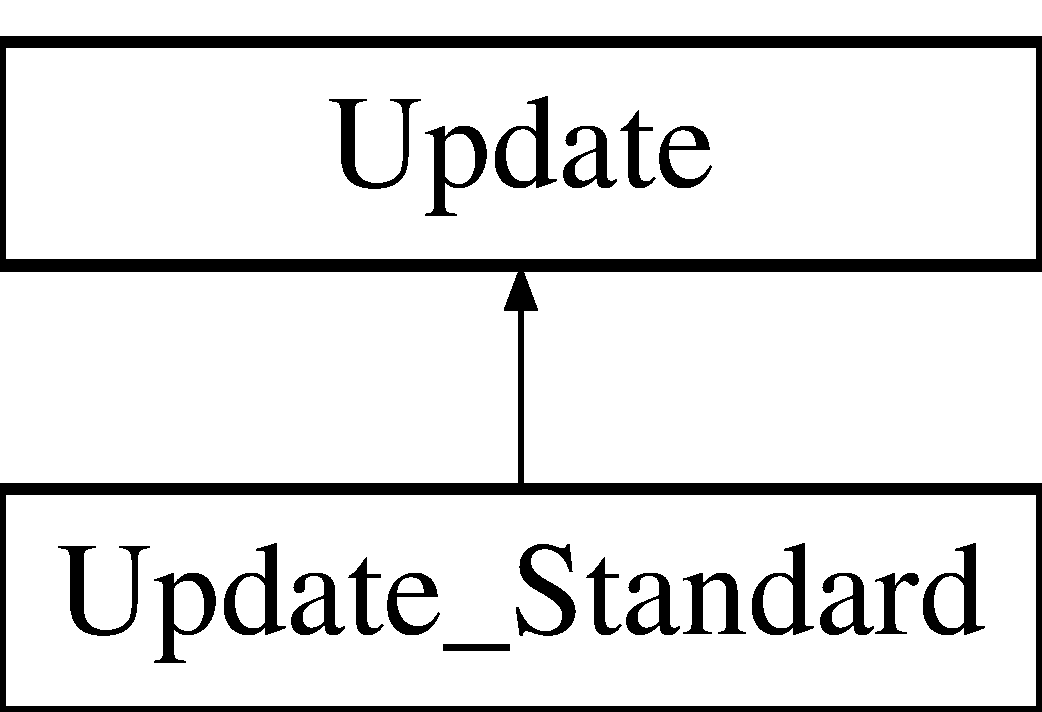
\includegraphics[height=2.000000cm]{class_update}
\end{center}
\end{figure}
\subsection*{Public Member Functions}
\begin{DoxyCompactItemize}
\item 
virtual \hyperlink{class_update_a08e4d08d01520e03e99e6d7a9a741726}{$\sim$\+Update} ()
\item 
virtual void \hyperlink{class_update_ae48a452118ffbc96c67c475182ae69a9}{operator()} (\hyperlink{class_grid}{Grid} $\ast$g, double dt, double weight=0) const =0
\end{DoxyCompactItemize}


\subsection{Detailed Description}
Abstract class for the update of a grid object during a time loop. 

\subsection{Constructor \& Destructor Documentation}
\index{Update@{Update}!````~Update@{$\sim$\+Update}}
\index{````~Update@{$\sim$\+Update}!Update@{Update}}
\subsubsection[{\texorpdfstring{$\sim$\+Update()}{~Update()}}]{\setlength{\rightskip}{0pt plus 5cm}virtual Update\+::$\sim$\+Update (
\begin{DoxyParamCaption}
{}
\end{DoxyParamCaption}
)\hspace{0.3cm}{\ttfamily [inline]}, {\ttfamily [virtual]}}\hypertarget{class_update_a08e4d08d01520e03e99e6d7a9a741726}{}\label{class_update_a08e4d08d01520e03e99e6d7a9a741726}


\subsection{Member Function Documentation}
\index{Update@{Update}!operator()@{operator()}}
\index{operator()@{operator()}!Update@{Update}}
\subsubsection[{\texorpdfstring{operator()(\+Grid $\ast$g, double dt, double weight=0) const =0}{operator()(Grid *g, double dt, double weight=0) const =0}}]{\setlength{\rightskip}{0pt plus 5cm}virtual void Update\+::operator() (
\begin{DoxyParamCaption}
\item[{{\bf Grid} $\ast$}]{g, }
\item[{double}]{dt, }
\item[{double}]{weight = {\ttfamily 0}}
\end{DoxyParamCaption}
) const\hspace{0.3cm}{\ttfamily [pure virtual]}}\hypertarget{class_update_ae48a452118ffbc96c67c475182ae69a9}{}\label{class_update_ae48a452118ffbc96c67c475182ae69a9}
\hyperlink{class_update}{Update} operator. 
\begin{DoxyParams}{Parameters}
{\em g} & grid \\
\hline
{\em dt} & time step \\
\hline
{\em weight} & weighting factor for the equation right-\/hand side (e.\+g. used in Runge-\/\+Kutta schemes) \\
\hline
\end{DoxyParams}


Implemented in \hyperlink{class_update___standard_aaea6d678d4e04d3a28e4e9e89b4a8f3f}{Update\+\_\+\+Standard}.



The documentation for this class was generated from the following file\+:\begin{DoxyCompactItemize}
\item 
/home/doberle/\+Advanced C\+F\+D/acfd/\+Code/\hyperlink{update_8h}{update.\+h}\end{DoxyCompactItemize}

\hypertarget{class_update___standard}{}\section{Update\+\_\+\+Standard Class Reference}
\label{class_update___standard}\index{Update\+\_\+\+Standard@{Update\+\_\+\+Standard}}


Class for the update of a grid object during a time loop, using standard flux differencing.  




{\ttfamily \#include $<$update\+\_\+standard.\+h$>$}

Inheritance diagram for Update\+\_\+\+Standard\+:\begin{figure}[H]
\begin{center}
\leavevmode
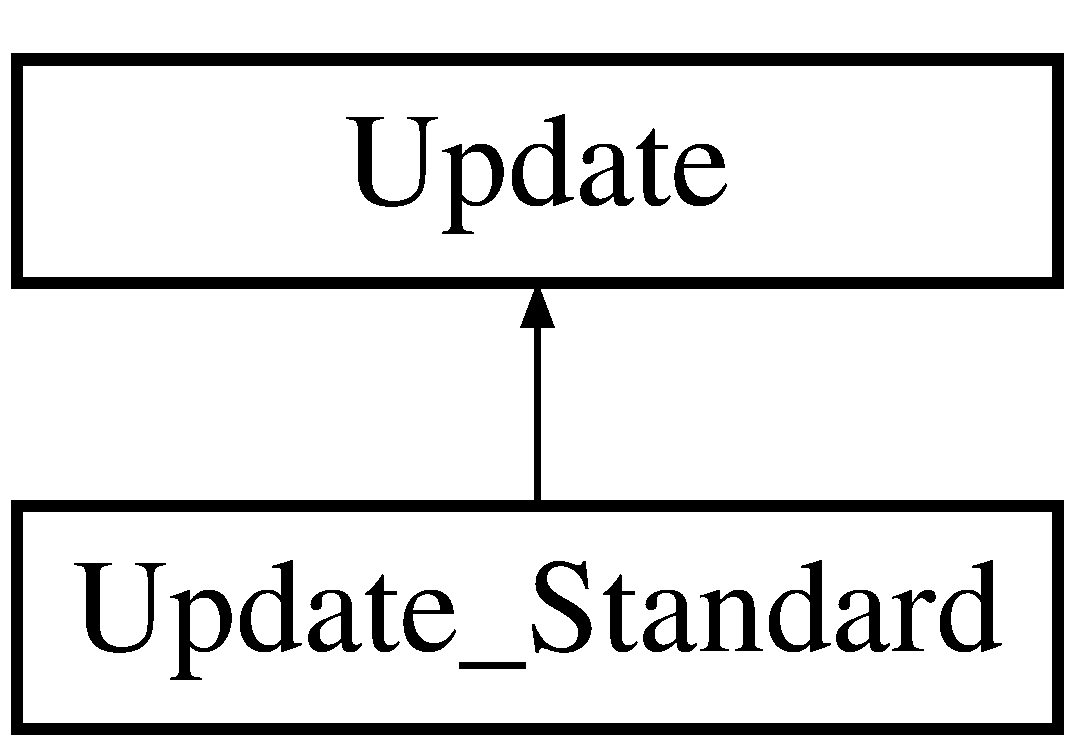
\includegraphics[height=2.000000cm]{class_update___standard}
\end{center}
\end{figure}
\subsection*{Public Member Functions}
\begin{DoxyCompactItemize}
\item 
void \hyperlink{class_update___standard_aaea6d678d4e04d3a28e4e9e89b4a8f3f}{operator()} (\hyperlink{class_grid}{Grid} $\ast$g, double dt, double weight=0) const 
\end{DoxyCompactItemize}


\subsection{Detailed Description}
Class for the update of a grid object during a time loop, using standard flux differencing. 

\subsection{Member Function Documentation}
\index{Update\+\_\+\+Standard@{Update\+\_\+\+Standard}!operator()@{operator()}}
\index{operator()@{operator()}!Update\+\_\+\+Standard@{Update\+\_\+\+Standard}}
\subsubsection[{\texorpdfstring{operator()(\+Grid $\ast$g, double dt, double weight=0) const }{operator()(Grid *g, double dt, double weight=0) const }}]{\setlength{\rightskip}{0pt plus 5cm}void Update\+\_\+\+Standard\+::operator() (
\begin{DoxyParamCaption}
\item[{{\bf Grid} $\ast$}]{g, }
\item[{double}]{dt, }
\item[{double}]{weight = {\ttfamily 0}}
\end{DoxyParamCaption}
) const\hspace{0.3cm}{\ttfamily [virtual]}}\hypertarget{class_update___standard_aaea6d678d4e04d3a28e4e9e89b4a8f3f}{}\label{class_update___standard_aaea6d678d4e04d3a28e4e9e89b4a8f3f}
\hyperlink{class_update}{Update} operator. 
\begin{DoxyParams}{Parameters}
{\em g} & grid \\
\hline
{\em dt} & time step \\
\hline
{\em weight} & weighting factor for the equation right-\/hand side (e.\+g. used in Runge-\/\+Kutta schemes) \\
\hline
\end{DoxyParams}


Implements \hyperlink{class_update_ae48a452118ffbc96c67c475182ae69a9}{Update}.



The documentation for this class was generated from the following files\+:\begin{DoxyCompactItemize}
\item 
/home/doberle/\+Advanced C\+F\+D/acfd/\+Code/\hyperlink{update__standard_8h}{update\+\_\+standard.\+h}\item 
/home/doberle/\+Advanced C\+F\+D/acfd/\+Code/\hyperlink{update__standard_8cpp}{update\+\_\+standard.\+cpp}\end{DoxyCompactItemize}

\chapter{File Documentation}
\hypertarget{boundary_8h}{}\section{/home/doberle/\+Advanced C\+F\+D/acfd/\+Code/boundary.h File Reference}
\label{boundary_8h}\index{/home/doberle/\+Advanced C\+F\+D/acfd/\+Code/boundary.\+h@{/home/doberle/\+Advanced C\+F\+D/acfd/\+Code/boundary.\+h}}
\subsection*{Classes}
\begin{DoxyCompactItemize}
\item 
class \hyperlink{class_boundary}{Boundary}
\begin{DoxyCompactList}\small\item\em Abstract class for the computation of boundary fluxes. \end{DoxyCompactList}\end{DoxyCompactItemize}

\hypertarget{boundary__periodic_8h}{}\section{/home/doberle/\+Advanced C\+F\+D/acfd/\+Code/boundary\+\_\+periodic.h File Reference}
\label{boundary__periodic_8h}\index{/home/doberle/\+Advanced C\+F\+D/acfd/\+Code/boundary\+\_\+periodic.\+h@{/home/doberle/\+Advanced C\+F\+D/acfd/\+Code/boundary\+\_\+periodic.\+h}}
{\ttfamily \#include \char`\"{}boundary.\+h\char`\"{}}\\*
{\ttfamily \#include \char`\"{}grid.\+h\char`\"{}}\\*
\subsection*{Classes}
\begin{DoxyCompactItemize}
\item 
class \hyperlink{class_boundary___periodic}{Boundary\+\_\+\+Periodic}
\begin{DoxyCompactList}\small\item\em Class for the computation of boundary fluxes for a periodic boundary condition. \end{DoxyCompactList}\end{DoxyCompactItemize}

\hypertarget{control_8cpp}{}\section{/home/doberle/\+Advanced C\+F\+D/acfd/\+Code/control.cpp File Reference}
\label{control_8cpp}\index{/home/doberle/\+Advanced C\+F\+D/acfd/\+Code/control.\+cpp@{/home/doberle/\+Advanced C\+F\+D/acfd/\+Code/control.\+cpp}}
{\ttfamily \#include \char`\"{}control.\+h\char`\"{}}\\*
{\ttfamily \#include $<$string$>$}\\*
{\ttfamily \#include $<$cstring$>$}\\*
{\ttfamily \#include $<$fstream$>$}\\*
{\ttfamily \#include $<$iostream$>$}\\*
{\ttfamily \#include $<$stdlib.\+h$>$}\\*

\hypertarget{control_8h}{}\section{/home/doberle/\+Advanced C\+F\+D/acfd/\+Code/control.h File Reference}
\label{control_8h}\index{/home/doberle/\+Advanced C\+F\+D/acfd/\+Code/control.\+h@{/home/doberle/\+Advanced C\+F\+D/acfd/\+Code/control.\+h}}
{\ttfamily \#include $<$map$>$}\\*
{\ttfamily \#include $<$string$>$}\\*
\subsection*{Classes}
\begin{DoxyCompactItemize}
\item 
class \hyperlink{class_control}{Control}
\begin{DoxyCompactList}\small\item\em Map that holds the contents of a control file. \end{DoxyCompactList}\item 
struct \hyperlink{struct_control_1_1_control_pair}{Control\+::\+Control\+Pair}
\end{DoxyCompactItemize}

\hypertarget{driver_8h}{}\section{/home/doberle/\+Advanced C\+F\+D/acfd/\+Code/driver.h File Reference}
\label{driver_8h}\index{/home/doberle/\+Advanced C\+F\+D/acfd/\+Code/driver.\+h@{/home/doberle/\+Advanced C\+F\+D/acfd/\+Code/driver.\+h}}
\subsection*{Classes}
\begin{DoxyCompactItemize}
\item 
class \hyperlink{class_driver}{Driver}
\begin{DoxyCompactList}\small\item\em Abstract class for a simulation code driver. \end{DoxyCompactList}\end{DoxyCompactItemize}

\hypertarget{driver__standard_8cpp}{}\section{/home/doberle/\+Advanced C\+F\+D/acfd/\+Code/driver\+\_\+standard.cpp File Reference}
\label{driver__standard_8cpp}\index{/home/doberle/\+Advanced C\+F\+D/acfd/\+Code/driver\+\_\+standard.\+cpp@{/home/doberle/\+Advanced C\+F\+D/acfd/\+Code/driver\+\_\+standard.\+cpp}}
{\ttfamily \#include \char`\"{}driver\+\_\+standard.\+h\char`\"{}}\\*
{\ttfamily \#include \char`\"{}control.\+h\char`\"{}}\\*
{\ttfamily \#include \char`\"{}time.\+h\char`\"{}}\\*
{\ttfamily \#include \char`\"{}init.\+h\char`\"{}}\\*
{\ttfamily \#include \char`\"{}boundary.\+h\char`\"{}}\\*
{\ttfamily \#include \char`\"{}fluxes.\+h\char`\"{}}\\*
{\ttfamily \#include \char`\"{}source.\+h\char`\"{}}\\*
{\ttfamily \#include \char`\"{}update.\+h\char`\"{}}\\*
{\ttfamily \#include \char`\"{}plot.\+h\char`\"{}}\\*
{\ttfamily \#include \char`\"{}setup\+\_\+advection.\+h\char`\"{}}\\*
{\ttfamily \#include $<$stdio.\+h$>$}\\*

\hypertarget{driver__standard_8h}{}\section{/home/doberle/\+Advanced C\+F\+D/acfd/\+Code/driver\+\_\+standard.h File Reference}
\label{driver__standard_8h}\index{/home/doberle/\+Advanced C\+F\+D/acfd/\+Code/driver\+\_\+standard.\+h@{/home/doberle/\+Advanced C\+F\+D/acfd/\+Code/driver\+\_\+standard.\+h}}
{\ttfamily \#include \char`\"{}driver.\+h\char`\"{}}\\*
\subsection*{Classes}
\begin{DoxyCompactItemize}
\item 
class \hyperlink{class_driver___standard}{Driver\+\_\+\+Standard}
\begin{DoxyCompactList}\small\item\em \hyperlink{class_driver}{Driver} for numerical simulation of conservation laws. \end{DoxyCompactList}\end{DoxyCompactItemize}

\hypertarget{fluxes_8cpp}{}\section{/home/doberle/\+Advanced C\+F\+D/acfd/\+Code/fluxes.cpp File Reference}
\label{fluxes_8cpp}\index{/home/doberle/\+Advanced C\+F\+D/acfd/\+Code/fluxes.\+cpp@{/home/doberle/\+Advanced C\+F\+D/acfd/\+Code/fluxes.\+cpp}}
{\ttfamily \#include \char`\"{}fluxes.\+h\char`\"{}}\\*
{\ttfamily \#include \char`\"{}control.\+h\char`\"{}}\\*
{\ttfamily \#include \char`\"{}grid.\+h\char`\"{}}\\*

\hypertarget{fluxes_8h}{}\section{/home/doberle/\+Advanced C\+F\+D/acfd/\+Code/fluxes.h File Reference}
\label{fluxes_8h}\index{/home/doberle/\+Advanced C\+F\+D/acfd/\+Code/fluxes.\+h@{/home/doberle/\+Advanced C\+F\+D/acfd/\+Code/fluxes.\+h}}
{\ttfamily \#include $<$math.\+h$>$}\\*
\subsection*{Classes}
\begin{DoxyCompactItemize}
\item 
class \hyperlink{class_fluxes}{Fluxes}
\begin{DoxyCompactList}\small\item\em Class for the computation of numerical fluxes over cell interfaces for a given conservation law. \end{DoxyCompactList}\end{DoxyCompactItemize}

\hypertarget{fluxes__advection_8cpp}{}\section{/home/doberle/\+Advanced C\+F\+D/acfd/\+Code/fluxes\+\_\+advection.cpp File Reference}
\label{fluxes__advection_8cpp}\index{/home/doberle/\+Advanced C\+F\+D/acfd/\+Code/fluxes\+\_\+advection.\+cpp@{/home/doberle/\+Advanced C\+F\+D/acfd/\+Code/fluxes\+\_\+advection.\+cpp}}
{\ttfamily \#include \char`\"{}fluxes\+\_\+advection.\+h\char`\"{}}\\*
{\ttfamily \#include \char`\"{}grid.\+h\char`\"{}}\\*

\hypertarget{fluxes__advection_8h}{}\section{/home/doberle/\+Advanced C\+F\+D/acfd/\+Code/fluxes\+\_\+advection.h File Reference}
\label{fluxes__advection_8h}\index{/home/doberle/\+Advanced C\+F\+D/acfd/\+Code/fluxes\+\_\+advection.\+h@{/home/doberle/\+Advanced C\+F\+D/acfd/\+Code/fluxes\+\_\+advection.\+h}}
{\ttfamily \#include \char`\"{}fluxes.\+h\char`\"{}}\\*
{\ttfamily \#include \char`\"{}control.\+h\char`\"{}}\\*
{\ttfamily \#include $<$stdio.\+h$>$}\\*
\subsection*{Classes}
\begin{DoxyCompactItemize}
\item 
class \hyperlink{class_fluxes___advection}{Fluxes\+\_\+\+Advection}
\begin{DoxyCompactList}\small\item\em Computation of fluxes for the linear advection-\/diffusion equation. \end{DoxyCompactList}\end{DoxyCompactItemize}

\hypertarget{gnuplot__i_8cpp}{}\section{/home/doberle/\+Advanced C\+F\+D/acfd/\+Code/gnuplot\+\_\+i.cpp File Reference}
\label{gnuplot__i_8cpp}\index{/home/doberle/\+Advanced C\+F\+D/acfd/\+Code/gnuplot\+\_\+i.\+cpp@{/home/doberle/\+Advanced C\+F\+D/acfd/\+Code/gnuplot\+\_\+i.\+cpp}}
{\ttfamily \#include \char`\"{}gnuplot\+\_\+i.\+h\char`\"{}}\\*
\subsection*{Macros}
\begin{DoxyCompactItemize}
\item 
\#define \hyperlink{gnuplot__i_8cpp_a98724840ca52cabedc31eb7a57aca57b}{P\+A\+T\+H\+\_\+\+M\+A\+X\+N\+A\+M\+E\+SZ}~4096
\end{DoxyCompactItemize}
\subsection*{Functions}
\begin{DoxyCompactItemize}
\item 
{\footnotesize template$<$typename Container $>$ }\\void \hyperlink{gnuplot__i_8cpp_a1a96d6f33e0d7225eaaf015313e53a4c}{stringtok} (Container \&container, string const \&in, const char $\ast$const delimiters=\char`\"{} \textbackslash{}t\textbackslash{}n\char`\"{})
\end{DoxyCompactItemize}


\subsection{Macro Definition Documentation}
\index{gnuplot\+\_\+i.\+cpp@{gnuplot\+\_\+i.\+cpp}!P\+A\+T\+H\+\_\+\+M\+A\+X\+N\+A\+M\+E\+SZ@{P\+A\+T\+H\+\_\+\+M\+A\+X\+N\+A\+M\+E\+SZ}}
\index{P\+A\+T\+H\+\_\+\+M\+A\+X\+N\+A\+M\+E\+SZ@{P\+A\+T\+H\+\_\+\+M\+A\+X\+N\+A\+M\+E\+SZ}!gnuplot\+\_\+i.\+cpp@{gnuplot\+\_\+i.\+cpp}}
\subsubsection[{\texorpdfstring{P\+A\+T\+H\+\_\+\+M\+A\+X\+N\+A\+M\+E\+SZ}{PATH_MAXNAMESZ}}]{\setlength{\rightskip}{0pt plus 5cm}\#define P\+A\+T\+H\+\_\+\+M\+A\+X\+N\+A\+M\+E\+SZ~4096}\hypertarget{gnuplot__i_8cpp_a98724840ca52cabedc31eb7a57aca57b}{}\label{gnuplot__i_8cpp_a98724840ca52cabedc31eb7a57aca57b}


\subsection{Function Documentation}
\index{gnuplot\+\_\+i.\+cpp@{gnuplot\+\_\+i.\+cpp}!stringtok@{stringtok}}
\index{stringtok@{stringtok}!gnuplot\+\_\+i.\+cpp@{gnuplot\+\_\+i.\+cpp}}
\subsubsection[{\texorpdfstring{stringtok(\+Container \&container, string const \&in, const char $\ast$const delimiters="" \textbackslash{}t\textbackslash{}n"")}{stringtok(Container &container, string const &in, const char *const delimiters=" \textbackslash{}t\textbackslash{}n")}}]{\setlength{\rightskip}{0pt plus 5cm}template$<$typename Container $>$ void stringtok (
\begin{DoxyParamCaption}
\item[{Container \&}]{container, }
\item[{string const \&}]{in, }
\item[{const char $\ast$const}]{delimiters = {\ttfamily \char`\"{}~\textbackslash{}t\textbackslash{}n\char`\"{}}}
\end{DoxyParamCaption}
)}\hypertarget{gnuplot__i_8cpp_a1a96d6f33e0d7225eaaf015313e53a4c}{}\label{gnuplot__i_8cpp_a1a96d6f33e0d7225eaaf015313e53a4c}

\hypertarget{gnuplot__i_8h}{}\section{/home/doberle/\+Advanced C\+F\+D/acfd/\+Code/gnuplot\+\_\+i.h File Reference}
\label{gnuplot__i_8h}\index{/home/doberle/\+Advanced C\+F\+D/acfd/\+Code/gnuplot\+\_\+i.\+h@{/home/doberle/\+Advanced C\+F\+D/acfd/\+Code/gnuplot\+\_\+i.\+h}}
{\ttfamily \#include $<$stdarg.\+h$>$}\\*
{\ttfamily \#include $<$unistd.\+h$>$}\\*
{\ttfamily \#include $<$cstdlib$>$}\\*
{\ttfamily \#include $<$cstdio$>$}\\*
{\ttfamily \#include $<$cstring$>$}\\*
{\ttfamily \#include $<$string$>$}\\*
{\ttfamily \#include $<$iostream$>$}\\*
{\ttfamily \#include $<$fstream$>$}\\*
{\ttfamily \#include $<$sstream$>$}\\*
{\ttfamily \#include $<$list$>$}\\*
{\ttfamily \#include $<$vector$>$}\\*
{\ttfamily \#include $<$stdexcept$>$}\\*
\subsection*{Classes}
\begin{DoxyCompactItemize}
\item 
class \hyperlink{class_gnuplot_exception}{Gnuplot\+Exception}
\item 
class \hyperlink{class_gnuplot}{Gnuplot}
\end{DoxyCompactItemize}
\subsection*{Macros}
\begin{DoxyCompactItemize}
\item 
\#define \hyperlink{gnuplot__i_8h_a0b92738856c4bda43003d1c847483dd2}{G\+P\+\_\+\+M\+A\+X\+\_\+\+T\+M\+P\+\_\+\+F\+I\+L\+ES}~64
\item 
\#define \hyperlink{gnuplot__i_8h_a093b4c5627360601a4605251ed3495c8}{G\+P\+\_\+\+T\+M\+P\+\_\+\+N\+A\+M\+E\+\_\+\+S\+I\+ZE}~512
\item 
\#define \hyperlink{gnuplot__i_8h_adc74c0a238dd6f2220b0b2839cdda632}{G\+P\+\_\+\+C\+M\+D\+\_\+\+S\+I\+ZE}~1024
\item 
\#define \hyperlink{gnuplot__i_8h_a9e47e543bc0b91c93c5d8d259c563977}{G\+P\+\_\+\+T\+I\+T\+L\+E\+\_\+\+S\+I\+ZE}~80
\end{DoxyCompactItemize}


\subsection{Macro Definition Documentation}
\index{gnuplot\+\_\+i.\+h@{gnuplot\+\_\+i.\+h}!G\+P\+\_\+\+C\+M\+D\+\_\+\+S\+I\+ZE@{G\+P\+\_\+\+C\+M\+D\+\_\+\+S\+I\+ZE}}
\index{G\+P\+\_\+\+C\+M\+D\+\_\+\+S\+I\+ZE@{G\+P\+\_\+\+C\+M\+D\+\_\+\+S\+I\+ZE}!gnuplot\+\_\+i.\+h@{gnuplot\+\_\+i.\+h}}
\subsubsection[{\texorpdfstring{G\+P\+\_\+\+C\+M\+D\+\_\+\+S\+I\+ZE}{GP_CMD_SIZE}}]{\setlength{\rightskip}{0pt plus 5cm}\#define G\+P\+\_\+\+C\+M\+D\+\_\+\+S\+I\+ZE~1024}\hypertarget{gnuplot__i_8h_adc74c0a238dd6f2220b0b2839cdda632}{}\label{gnuplot__i_8h_adc74c0a238dd6f2220b0b2839cdda632}
\index{gnuplot\+\_\+i.\+h@{gnuplot\+\_\+i.\+h}!G\+P\+\_\+\+M\+A\+X\+\_\+\+T\+M\+P\+\_\+\+F\+I\+L\+ES@{G\+P\+\_\+\+M\+A\+X\+\_\+\+T\+M\+P\+\_\+\+F\+I\+L\+ES}}
\index{G\+P\+\_\+\+M\+A\+X\+\_\+\+T\+M\+P\+\_\+\+F\+I\+L\+ES@{G\+P\+\_\+\+M\+A\+X\+\_\+\+T\+M\+P\+\_\+\+F\+I\+L\+ES}!gnuplot\+\_\+i.\+h@{gnuplot\+\_\+i.\+h}}
\subsubsection[{\texorpdfstring{G\+P\+\_\+\+M\+A\+X\+\_\+\+T\+M\+P\+\_\+\+F\+I\+L\+ES}{GP_MAX_TMP_FILES}}]{\setlength{\rightskip}{0pt plus 5cm}\#define G\+P\+\_\+\+M\+A\+X\+\_\+\+T\+M\+P\+\_\+\+F\+I\+L\+ES~64}\hypertarget{gnuplot__i_8h_a0b92738856c4bda43003d1c847483dd2}{}\label{gnuplot__i_8h_a0b92738856c4bda43003d1c847483dd2}
\index{gnuplot\+\_\+i.\+h@{gnuplot\+\_\+i.\+h}!G\+P\+\_\+\+T\+I\+T\+L\+E\+\_\+\+S\+I\+ZE@{G\+P\+\_\+\+T\+I\+T\+L\+E\+\_\+\+S\+I\+ZE}}
\index{G\+P\+\_\+\+T\+I\+T\+L\+E\+\_\+\+S\+I\+ZE@{G\+P\+\_\+\+T\+I\+T\+L\+E\+\_\+\+S\+I\+ZE}!gnuplot\+\_\+i.\+h@{gnuplot\+\_\+i.\+h}}
\subsubsection[{\texorpdfstring{G\+P\+\_\+\+T\+I\+T\+L\+E\+\_\+\+S\+I\+ZE}{GP_TITLE_SIZE}}]{\setlength{\rightskip}{0pt plus 5cm}\#define G\+P\+\_\+\+T\+I\+T\+L\+E\+\_\+\+S\+I\+ZE~80}\hypertarget{gnuplot__i_8h_a9e47e543bc0b91c93c5d8d259c563977}{}\label{gnuplot__i_8h_a9e47e543bc0b91c93c5d8d259c563977}
\index{gnuplot\+\_\+i.\+h@{gnuplot\+\_\+i.\+h}!G\+P\+\_\+\+T\+M\+P\+\_\+\+N\+A\+M\+E\+\_\+\+S\+I\+ZE@{G\+P\+\_\+\+T\+M\+P\+\_\+\+N\+A\+M\+E\+\_\+\+S\+I\+ZE}}
\index{G\+P\+\_\+\+T\+M\+P\+\_\+\+N\+A\+M\+E\+\_\+\+S\+I\+ZE@{G\+P\+\_\+\+T\+M\+P\+\_\+\+N\+A\+M\+E\+\_\+\+S\+I\+ZE}!gnuplot\+\_\+i.\+h@{gnuplot\+\_\+i.\+h}}
\subsubsection[{\texorpdfstring{G\+P\+\_\+\+T\+M\+P\+\_\+\+N\+A\+M\+E\+\_\+\+S\+I\+ZE}{GP_TMP_NAME_SIZE}}]{\setlength{\rightskip}{0pt plus 5cm}\#define G\+P\+\_\+\+T\+M\+P\+\_\+\+N\+A\+M\+E\+\_\+\+S\+I\+ZE~512}\hypertarget{gnuplot__i_8h_a093b4c5627360601a4605251ed3495c8}{}\label{gnuplot__i_8h_a093b4c5627360601a4605251ed3495c8}

\hypertarget{grid_8cpp}{}\section{/home/doberle/\+Advanced C\+F\+D/acfd/\+Code/grid.cpp File Reference}
\label{grid_8cpp}\index{/home/doberle/\+Advanced C\+F\+D/acfd/\+Code/grid.\+cpp@{/home/doberle/\+Advanced C\+F\+D/acfd/\+Code/grid.\+cpp}}
{\ttfamily \#include \char`\"{}grid.\+h\char`\"{}}\\*

\hypertarget{grid_8h}{}\section{/home/doberle/\+Advanced C\+F\+D/acfd/\+Code/grid.h File Reference}
\label{grid_8h}\index{/home/doberle/\+Advanced C\+F\+D/acfd/\+Code/grid.\+h@{/home/doberle/\+Advanced C\+F\+D/acfd/\+Code/grid.\+h}}
\subsection*{Classes}
\begin{DoxyCompactItemize}
\item 
class \hyperlink{class_grid}{Grid}
\begin{DoxyCompactList}\small\item\em Class for a 3D Cartesian grid with associated fields and coefficients. \end{DoxyCompactList}\end{DoxyCompactItemize}

\hypertarget{init_8h}{}\section{/home/doberle/\+Advanced C\+F\+D/acfd/\+Code/init.h File Reference}
\label{init_8h}\index{/home/doberle/\+Advanced C\+F\+D/acfd/\+Code/init.\+h@{/home/doberle/\+Advanced C\+F\+D/acfd/\+Code/init.\+h}}
{\ttfamily \#include \char`\"{}control.\+h\char`\"{}}\\*
\subsection*{Classes}
\begin{DoxyCompactItemize}
\item 
class \hyperlink{class_init}{Init}
\begin{DoxyCompactList}\small\item\em Abstract class for the definition of initial conditions for fields defined on a \hyperlink{class_grid}{Grid} object. \end{DoxyCompactList}\end{DoxyCompactItemize}

\hypertarget{init__advection_8cpp}{}\section{/home/doberle/\+Advanced C\+F\+D/acfd/\+Code/init\+\_\+advection.cpp File Reference}
\label{init__advection_8cpp}\index{/home/doberle/\+Advanced C\+F\+D/acfd/\+Code/init\+\_\+advection.\+cpp@{/home/doberle/\+Advanced C\+F\+D/acfd/\+Code/init\+\_\+advection.\+cpp}}
{\ttfamily \#include \char`\"{}init\+\_\+advection.\+h\char`\"{}}\\*
{\ttfamily \#include \char`\"{}grid.\+h\char`\"{}}\\*
{\ttfamily \#include $<$math.\+h$>$}\\*

\hypertarget{init__advection_8h}{}\section{/home/doberle/\+Advanced C\+F\+D/acfd/\+Code/init\+\_\+advection.h File Reference}
\label{init__advection_8h}\index{/home/doberle/\+Advanced C\+F\+D/acfd/\+Code/init\+\_\+advection.\+h@{/home/doberle/\+Advanced C\+F\+D/acfd/\+Code/init\+\_\+advection.\+h}}
{\ttfamily \#include \char`\"{}init.\+h\char`\"{}}\\*
{\ttfamily \#include $<$stdio.\+h$>$}\\*
\subsection*{Classes}
\begin{DoxyCompactItemize}
\item 
class \hyperlink{class_init___advection}{Init\+\_\+\+Advection}
\begin{DoxyCompactList}\small\item\em Initial condition for the linear advection-\/diffusion equation. \end{DoxyCompactList}\end{DoxyCompactItemize}

\hypertarget{main_8cpp}{}\section{/home/doberle/\+Advanced C\+F\+D/acfd/\+Code/main.cpp File Reference}
\label{main_8cpp}\index{/home/doberle/\+Advanced C\+F\+D/acfd/\+Code/main.\+cpp@{/home/doberle/\+Advanced C\+F\+D/acfd/\+Code/main.\+cpp}}
{\ttfamily \#include \char`\"{}driver\+\_\+standard.\+h\char`\"{}}\\*
\subsection*{Functions}
\begin{DoxyCompactItemize}
\item 
int \hyperlink{main_8cpp_af3ed9c200de85b53c94cd18764b246a2}{main} (int argc, char $\ast$const argv\mbox{[}$\,$\mbox{]})
\end{DoxyCompactItemize}


\subsection{Function Documentation}
\index{main.\+cpp@{main.\+cpp}!main@{main}}
\index{main@{main}!main.\+cpp@{main.\+cpp}}
\subsubsection[{\texorpdfstring{main(int argc, char $\ast$const argv[])}{main(int argc, char *const argv[])}}]{\setlength{\rightskip}{0pt plus 5cm}int main (
\begin{DoxyParamCaption}
\item[{int}]{argc, }
\item[{char $\ast$const}]{argv\mbox{[}$\,$\mbox{]}}
\end{DoxyParamCaption}
)}\hypertarget{main_8cpp_af3ed9c200de85b53c94cd18764b246a2}{}\label{main_8cpp_af3ed9c200de85b53c94cd18764b246a2}

\hypertarget{plot_8h}{}\section{/home/doberle/\+Advanced C\+F\+D/acfd/\+Code/plot.h File Reference}
\label{plot_8h}\index{/home/doberle/\+Advanced C\+F\+D/acfd/\+Code/plot.\+h@{/home/doberle/\+Advanced C\+F\+D/acfd/\+Code/plot.\+h}}
\subsection*{Classes}
\begin{DoxyCompactItemize}
\item 
class \hyperlink{class_plot}{Plot}
\begin{DoxyCompactList}\small\item\em Abstract class for plotting simulation results. \end{DoxyCompactList}\end{DoxyCompactItemize}

\hypertarget{plot__advection_8cpp}{}\section{/home/doberle/\+Advanced C\+F\+D/acfd/\+Code/plot\+\_\+advection.cpp File Reference}
\label{plot__advection_8cpp}\index{/home/doberle/\+Advanced C\+F\+D/acfd/\+Code/plot\+\_\+advection.\+cpp@{/home/doberle/\+Advanced C\+F\+D/acfd/\+Code/plot\+\_\+advection.\+cpp}}
{\ttfamily \#include \char`\"{}plot\+\_\+advection.\+h\char`\"{}}\\*
{\ttfamily \#include \char`\"{}grid.\+h\char`\"{}}\\*

\hypertarget{plot__advection_8h}{}\section{/home/doberle/\+Advanced C\+F\+D/acfd/\+Code/plot\+\_\+advection.h File Reference}
\label{plot__advection_8h}\index{/home/doberle/\+Advanced C\+F\+D/acfd/\+Code/plot\+\_\+advection.\+h@{/home/doberle/\+Advanced C\+F\+D/acfd/\+Code/plot\+\_\+advection.\+h}}
{\ttfamily \#include \char`\"{}plot.\+h\char`\"{}}\\*
{\ttfamily \#include \char`\"{}control.\+h\char`\"{}}\\*
{\ttfamily \#include \char`\"{}gnuplot\+\_\+i.\+h\char`\"{}}\\*
{\ttfamily \#include $<$stdio.\+h$>$}\\*
\subsection*{Classes}
\begin{DoxyCompactItemize}
\item 
class \hyperlink{class_plot___advection}{Plot\+\_\+\+Advection}
\begin{DoxyCompactList}\small\item\em Plotting class for the linear advection-\/diffusion equation. \end{DoxyCompactList}\end{DoxyCompactItemize}

\hypertarget{postprocess_8h}{}\section{/home/doberle/\+Advanced C\+F\+D/acfd/\+Code/postprocess.h File Reference}
\label{postprocess_8h}\index{/home/doberle/\+Advanced C\+F\+D/acfd/\+Code/postprocess.\+h@{/home/doberle/\+Advanced C\+F\+D/acfd/\+Code/postprocess.\+h}}
\subsection*{Classes}
\begin{DoxyCompactItemize}
\item 
class \hyperlink{class_postprocess}{Postprocess}
\begin{DoxyCompactList}\small\item\em Abstract class for postprocessing simulation results. \end{DoxyCompactList}\end{DoxyCompactItemize}

\hypertarget{postprocess__advection_8cpp}{}\section{/home/doberle/\+Advanced C\+F\+D/acfd/\+Code/postprocess\+\_\+advection.cpp File Reference}
\label{postprocess__advection_8cpp}\index{/home/doberle/\+Advanced C\+F\+D/acfd/\+Code/postprocess\+\_\+advection.\+cpp@{/home/doberle/\+Advanced C\+F\+D/acfd/\+Code/postprocess\+\_\+advection.\+cpp}}
{\ttfamily \#include \char`\"{}postprocess\+\_\+advection.\+h\char`\"{}}\\*
{\ttfamily \#include \char`\"{}grid.\+h\char`\"{}}\\*
{\ttfamily \#include $<$cmath$>$}\\*
{\ttfamily \#include $<$stdio.\+h$>$}\\*

\hypertarget{postprocess__advection_8h}{}\section{/home/doberle/\+Advanced C\+F\+D/acfd/\+Code/postprocess\+\_\+advection.h File Reference}
\label{postprocess__advection_8h}\index{/home/doberle/\+Advanced C\+F\+D/acfd/\+Code/postprocess\+\_\+advection.\+h@{/home/doberle/\+Advanced C\+F\+D/acfd/\+Code/postprocess\+\_\+advection.\+h}}
{\ttfamily \#include \char`\"{}control.\+h\char`\"{}}\\*
{\ttfamily \#include \char`\"{}postprocess.\+h\char`\"{}}\\*
{\ttfamily \#include $<$stdio.\+h$>$}\\*
{\ttfamily \#include $<$cmath$>$}\\*
\subsection*{Classes}
\begin{DoxyCompactItemize}
\item 
class \hyperlink{class_postprocess___advection}{Postprocess\+\_\+\+Advection}
\begin{DoxyCompactList}\small\item\em Postprocessing class for the linear advection-\/diffusion equation. \end{DoxyCompactList}\end{DoxyCompactItemize}

\hypertarget{postprocess__empty_8h}{}\section{/home/doberle/\+Advanced C\+F\+D/acfd/\+Code/postprocess\+\_\+empty.h File Reference}
\label{postprocess__empty_8h}\index{/home/doberle/\+Advanced C\+F\+D/acfd/\+Code/postprocess\+\_\+empty.\+h@{/home/doberle/\+Advanced C\+F\+D/acfd/\+Code/postprocess\+\_\+empty.\+h}}
{\ttfamily \#include \char`\"{}postprocess.\+h\char`\"{}}\\*
\subsection*{Classes}
\begin{DoxyCompactItemize}
\item 
class \hyperlink{class_postprocess___empty}{Postprocess\+\_\+\+Empty}
\begin{DoxyCompactList}\small\item\em Empty postprocessing class (does nothing) \end{DoxyCompactList}\end{DoxyCompactItemize}

\hypertarget{setup_8h}{}\section{/home/doberle/\+Advanced C\+F\+D/acfd/\+Code/setup.h File Reference}
\label{setup_8h}\index{/home/doberle/\+Advanced C\+F\+D/acfd/\+Code/setup.\+h@{/home/doberle/\+Advanced C\+F\+D/acfd/\+Code/setup.\+h}}
{\ttfamily \#include \char`\"{}control.\+h\char`\"{}}\\*
{\ttfamily \#include \char`\"{}grid.\+h\char`\"{}}\\*
{\ttfamily \#include \char`\"{}time.\+h\char`\"{}}\\*
{\ttfamily \#include \char`\"{}postprocess.\+h\char`\"{}}\\*
{\ttfamily \#include $<$stdio.\+h$>$}\\*
\subsection*{Classes}
\begin{DoxyCompactItemize}
\item 
class \hyperlink{class_setup}{Setup}
\begin{DoxyCompactList}\small\item\em Class for the simulation setup. \end{DoxyCompactList}\end{DoxyCompactItemize}

\hypertarget{setup__advection_8h}{}\section{/home/doberle/\+Advanced C\+F\+D/acfd/\+Code/setup\+\_\+advection.h File Reference}
\label{setup__advection_8h}\index{/home/doberle/\+Advanced C\+F\+D/acfd/\+Code/setup\+\_\+advection.\+h@{/home/doberle/\+Advanced C\+F\+D/acfd/\+Code/setup\+\_\+advection.\+h}}
{\ttfamily \#include \char`\"{}setup.\+h\char`\"{}}\\*
{\ttfamily \#include \char`\"{}init\+\_\+advection.\+h\char`\"{}}\\*
{\ttfamily \#include \char`\"{}boundary\+\_\+periodic.\+h\char`\"{}}\\*
{\ttfamily \#include \char`\"{}fluxes\+\_\+advection.\+h\char`\"{}}\\*
{\ttfamily \#include \char`\"{}source\+\_\+empty.\+h\char`\"{}}\\*
{\ttfamily \#include \char`\"{}update\+\_\+standard.\+h\char`\"{}}\\*
{\ttfamily \#include \char`\"{}plot\+\_\+advection.\+h\char`\"{}}\\*
{\ttfamily \#include \char`\"{}postprocess\+\_\+advection.\+h\char`\"{}}\\*
\subsection*{Classes}
\begin{DoxyCompactItemize}
\item 
class \hyperlink{class_setup___advection}{Setup\+\_\+\+Advection}
\begin{DoxyCompactList}\small\item\em Simulation setup for the linear advection-\/diffusion equation. \end{DoxyCompactList}\end{DoxyCompactItemize}

\hypertarget{source_8h}{}\section{/home/doberle/\+Advanced C\+F\+D/acfd/\+Code/source.h File Reference}
\label{source_8h}\index{/home/doberle/\+Advanced C\+F\+D/acfd/\+Code/source.\+h@{/home/doberle/\+Advanced C\+F\+D/acfd/\+Code/source.\+h}}
{\ttfamily \#include \char`\"{}grid.\+h\char`\"{}}\\*
\subsection*{Classes}
\begin{DoxyCompactItemize}
\item 
class \hyperlink{class_source}{Source}
\begin{DoxyCompactList}\small\item\em Abstract class for a source term that is applied to a \hyperlink{class_grid}{Grid} object. \end{DoxyCompactList}\end{DoxyCompactItemize}

\hypertarget{source__empty_8h}{}\section{/home/doberle/\+Advanced C\+F\+D/acfd/\+Code/source\+\_\+empty.h File Reference}
\label{source__empty_8h}\index{/home/doberle/\+Advanced C\+F\+D/acfd/\+Code/source\+\_\+empty.\+h@{/home/doberle/\+Advanced C\+F\+D/acfd/\+Code/source\+\_\+empty.\+h}}
{\ttfamily \#include \char`\"{}source.\+h\char`\"{}}\\*
\subsection*{Classes}
\begin{DoxyCompactItemize}
\item 
class \hyperlink{class_source___empty}{Source\+\_\+\+Empty}
\begin{DoxyCompactList}\small\item\em Empty source, i.\+e., the source term equals zero. \end{DoxyCompactList}\end{DoxyCompactItemize}

\hypertarget{time_8h}{}\section{/home/doberle/\+Advanced C\+F\+D/acfd/\+Code/time.h File Reference}
\label{time_8h}\index{/home/doberle/\+Advanced C\+F\+D/acfd/\+Code/time.\+h@{/home/doberle/\+Advanced C\+F\+D/acfd/\+Code/time.\+h}}
\subsection*{Classes}
\begin{DoxyCompactItemize}
\item 
class \hyperlink{class_time}{Time}
\begin{DoxyCompactList}\small\item\em Class for running time loops. \end{DoxyCompactList}\end{DoxyCompactItemize}

\hypertarget{update_8h}{}\section{/home/doberle/\+Advanced C\+F\+D/acfd/\+Code/update.h File Reference}
\label{update_8h}\index{/home/doberle/\+Advanced C\+F\+D/acfd/\+Code/update.\+h@{/home/doberle/\+Advanced C\+F\+D/acfd/\+Code/update.\+h}}
\subsection*{Classes}
\begin{DoxyCompactItemize}
\item 
class \hyperlink{class_update}{Update}
\begin{DoxyCompactList}\small\item\em Abstract class for the update of a grid object during a time loop. \end{DoxyCompactList}\end{DoxyCompactItemize}

\hypertarget{update__standard_8cpp}{}\section{/home/doberle/\+Advanced C\+F\+D/acfd/\+Code/update\+\_\+standard.cpp File Reference}
\label{update__standard_8cpp}\index{/home/doberle/\+Advanced C\+F\+D/acfd/\+Code/update\+\_\+standard.\+cpp@{/home/doberle/\+Advanced C\+F\+D/acfd/\+Code/update\+\_\+standard.\+cpp}}
{\ttfamily \#include \char`\"{}update\+\_\+standard.\+h\char`\"{}}\\*
{\ttfamily \#include \char`\"{}grid.\+h\char`\"{}}\\*
{\ttfamily \#include $<$stdio.\+h$>$}\\*

\hypertarget{update__standard_8h}{}\section{/home/doberle/\+Advanced C\+F\+D/acfd/\+Code/update\+\_\+standard.h File Reference}
\label{update__standard_8h}\index{/home/doberle/\+Advanced C\+F\+D/acfd/\+Code/update\+\_\+standard.\+h@{/home/doberle/\+Advanced C\+F\+D/acfd/\+Code/update\+\_\+standard.\+h}}
{\ttfamily \#include \char`\"{}update.\+h\char`\"{}}\\*
\subsection*{Classes}
\begin{DoxyCompactItemize}
\item 
class \hyperlink{class_update___standard}{Update\+\_\+\+Standard}
\begin{DoxyCompactList}\small\item\em Class for the update of a grid object during a time loop, using standard flux differencing. \end{DoxyCompactList}\end{DoxyCompactItemize}

%--- End generated contents ---

% Index
\backmatter
\newpage
\phantomsection
\clearemptydoublepage
\addcontentsline{toc}{chapter}{Index}
\printindex

\end{document}
